\documentclass[11pt,twoside]{article}
\usepackage{fancyhdr}
\usepackage[colorlinks,citecolor=blue,urlcolor=blue,linkcolor=blue,bookmarks=false]{hyperref}
\usepackage{amsfonts,epsfig,graphicx}
\usepackage{afterpage}
\usepackage{amsmath,amssymb,amsthm} 
\usepackage{fullpage}
\usepackage[T1]{fontenc} 
\usepackage{epsf} 
\usepackage{graphics} 
\usepackage{amsfonts,amsmath}
\usepackage[sort,numbers]{natbib} 
\usepackage{psfrag,xspace}
\usepackage{color,etoolbox}

\setlength{\textwidth}{\paperwidth}
\addtolength{\textwidth}{-6cm}
\setlength{\textheight}{\paperheight}
\addtolength{\textheight}{-4cm}
\addtolength{\textheight}{-1.1\headheight}
\addtolength{\textheight}{-\headsep}
\addtolength{\textheight}{-\footskip}
\setlength{\oddsidemargin}{0.5cm}
\setlength{\evensidemargin}{0.5cm}

\newtheorem{theorem}{Theorem} 
\newtheorem{lemma}{Lemma}
\newtheorem{proposition}{Proposition}
\newtheorem{corollary}{Corollary}
\newtheorem{definition}{Definition}
\newtheorem*{remark}{Remark}

\usepackage[utf8]{inputenc} % allow utf-8 input
\usepackage[T1]{fontenc}    % use 8-bit T1 fonts
\usepackage{hyperref}       % hyperlinks
\usepackage{url}            % simple URL typesetting
\usepackage{booktabs}       % professional-quality tables
\usepackage{amsfonts}       % blackboard math symbols
\usepackage{nicefrac}       % compact symbols for 1/2, etc.
\usepackage{microtype}      % microtypography

\usepackage{microtype}
\usepackage{graphicx}
\usepackage{float}
\usepackage[export]{adjustbox}
\usepackage{subcaption}
\usepackage{booktabs}
\usepackage{xcolor}
%\usepackage{xr-hyper}
%\usepackage{hyperref}
%\usepackage[reqno]{amsmath}
%\usepackage{amsfonts, amsthm, amssymb}
\usepackage{algorithm}
\usepackage{algorithmic}
%\usepackage[parfill]{parskip}
\usepackage{enumerate}
\usepackage[shortlabels]{enumitem}
\usepackage{bm}
\usepackage{mathtools}

%%%%%% Begin Alden
\DeclarePairedDelimiter\abs{\lvert}{\rvert}

\newcommand{\diam}{\rho}
\newcommand{\set}[1]{\left\{#1\right\}}
\newcommand{\seq}[1]{\left\{#1\right\}_{n \in \mathbb{N}}}
\newcommand{\defeq}{\overset{\mathrm{def}}{=}}
\newcommand{\vol}{\mathrm{vol}}
\newcommand{\cut}{\mathrm{cut}}
% \newcommand{\abs}[1]{\left \lvert #1 \right \rvert}
\newcommand{\N}{\mathbb{N}}
\newcommand{\Reals}{\mathbb{R}}
\newcommand{\Rd}{\Reals^d}
\newcommand{\norm}[1]{\left\lVert#1\right\rVert}
\newcommand{\1}{\mathbf{1}}
\newcommand{\Phibf}{\Phi_{u}}
\newcommand{\Psibf}{\Psi_{u}}
\newcommand{\taubf}{\tau_{u}}
\newcommand{\dist}{\mathrm{dist}}
\newcommand{\Err}{\mathrm{Err}}
\newcommand{\TV}{\mathrm{TV}}

%%% Vectors
\newcommand{\pbf}{p}        % removed bold font
\newcommand{\qbf}{\mathbf{q}}
\newcommand{\ebf}[1]{{e}_{#1}}
\newcommand{\pibf}{\bm{\pi}}

%%% Matrices (no bold font)
\newcommand{\Abf}{A}
\newcommand{\Xbf}{X}             % removed bold font 
\newcommand{\Wbf}{W}
\newcommand{\Lbf}{L}
\newcommand{\Dbf}{D}
\newcommand{\Ibf}[1]{I_{#1}}

%%% Probability distributions (and related items)
\newcommand{\Pbb}{\mathbb{P}}
\newcommand{\Cbb}{\mathbb{C}}
\newcommand{\Ebb}{\mathbb{E}}

%%% Sets
\newcommand{\Sset}{\mathcal{S}}
\newcommand{\Cset}{\mathcal{C}}
\newcommand{\Aset}{\mathcal{A}}
\newcommand{\Asig}{\Aset_{\sigma}}
\newcommand{\Csig}{\Cset_{\sigma}}
\newcommand{\Asigr}{\Aset_{\sigma,\sigma + r}}
\newcommand{\Csigr}{\Cset_{\sigma,\sigma + r}}

%%% Graph quantities
\newcommand{\Cest}{\widehat{C}}
\newcommand{\degminpr}{\deg_{\min}'}
\newcommand{\degminwt}{\widetilde{\deg}_{\min}}
\newcommand{\degmaxwt}{\widetilde{\deg}_{\max}}
\newcommand{\degmax}{\deg_{\max}}
\newcommand{\piminwt}{\widetilde{\pi}_{\min}}
\newcommand{\piminpr}{\pibf_{\min}'}
\newcommand{\degmin}{\deg_{\min}}

%%% Operators
\DeclareMathOperator*{\argmin}{arg\,min}
\newcommand{\dx}{\,dx}
\newcommand{\dy}{\,dy}
\newcommand{\dt}{\,dt}

%%% Algorithm notation
\newcommand{\ppr}{{\sc PPR}}
\newcommand{\pprspace}{{\sc PPR~}}

%%% Tilde notation for quantities over the expansion set 
\newcommand{\wn}{\widetilde{n}}
\newcommand{\wX}{\widetilde{\Xbf}}
\newcommand{\wx}{\widetilde{x}}
\newcommand{\wz}{\widetilde{z}}
\newcommand{\wbz}{\widetilde{\bf{z}}}
\newcommand{\wu}{\widetilde{u}}
\newcommand{\wPbb}{\widetilde{\Pbb}}
\newcommand{\wf}{\widetilde{f}}
\newcommand{\wDbf}{\widetilde{\Dbf}}
\newcommand{\piwt}{\widetilde{\pi}}

\newcommand{\sbcomment}[1]{{\color{red} \bf{{{{SB --- #1}}}}}}

%\newtheoremstyle{aldenthm}
%{6pt} % Space above
%{6pt} % Space below
%{\itshape} % Body font
%{} % Indent amount
%{\bfseries} % Theorem head font
%{.} % Punctuation after theorem head
%{.5em} % Space after theorem head
%{} % Theorem head spec (can be left empty, meaning `normal')

%\theoremstyle{aldenthm}
%\newtheorem{theorem}{Theorem}
%\newtheorem{definition}{Definition}
%\newtheorem{lemma}{Lemma}
%\newtheorem{proposition}{Proposition}
%\newtheorem{corollary}{Corollary}

%\newtheoremstyle{aldenrmrk}
%{6pt} % Space above
%{6pt} % Space below
%{} % Body font
%{} % Indent amount
%{\itshape} % Theorem head font
%{.} % Punctuation after theorem head
%{.5em} % Space after theorem head
%{} % Theorem head spec (can be left empty, meaning `normal')
%
%\theoremstyle{aldenrmrk}
%\newtheorem{remark}{Remark}
%%%%%% End Alden

%\title{Local Spectral Clustering of Density Upper Level Sets}

% The \author macro works with any number of authors. There are two commands
% used to separate the names and addresses of multiple authors: \And and \AND.
%
% Using \And between authors leaves it to LaTeX to determine where to break the
% lines. Using \AND forces a line break at that point. So, if LaTeX puts 3 of 4
% authors names on the first line, and the last on the second line, try using
% \AND instead of \And before the third author name.
%
%\author{
%Alden Green \And
%Sivaraman Balakrishnan \And
%Ryan J. Tibshirani}
%
%\begin{document}
%\maketitle
%
%\vspace{0.1in}
%\begin{abstract}


\newcommand{\widgraph}[2]{\includegraphics[keepaspectratio,width=#1]{#2}}
\newcommand{\Like}{\ensuremath{\mathcal{L}}}
\newcommand{\Ball}[2]{\mathbb{B}_{#1}(#2)}
\newcommand{\Complement}[1]{\overline{#1}}

\newcommand{\xsam}{\ensuremath{x}}
\newcommand{\samind}{\ensuremath{\ell}}
\newcommand{\Xrv}{\ensuremath{X}}
\newcommand{\Event}{\ensuremath{\mathcal{E}}}
\newcommand{\Fevent}{\ensuremath{\mathcal{F}}}

\newcommand{\usedim}{\ensuremath{d}}
\newcommand{\mubold}{\ensuremath{\boldsymbol{\mu}}}
\newcommand{\lambold}{\ensuremath{\boldsymbol{\lambda}}}
\newcommand{\sep}{\ensuremath{\xi}}
\newcommand{\mixind}{\ensuremath{i}}
\newcommand{\mixtwo}{\ensuremath{j}}
\newcommand{\nummix}{\ensuremath{M}}
\newcommand{\mustar}{\ensuremath{\mu^*}}
\newcommand{\muboldstar}{\ensuremath{\mubold^*}}
\newcommand{\muboldt}{\ensuremath{\mubold^t}}

\newcommand{\numobs}{\ensuremath{n}}
\newcommand{\SamLike}{\ensuremath{\Like_\numobs}}
\newcommand{\PopLike}{\ensuremath{\Like}}
\newcommand{\Exs}{\E}
\newcommand{\thetanew}{\ensuremath{\theta^{\text{\small{new}} }}}

\newcommand{\stepsize}{\ensuremath{s}}


\newcommand{\QMAT}{\ensuremath{\mathbf{Q}}} 
\newcommand{\DMAT}{\ensuremath{\mathbf{D}}} 

\newcommand{\defn}{\ensuremath{: \, =}}
\newcommand{\muboldtilde}{\ensuremath{\tilde{\mubold}}}

%%% New version of \caption puts things in smaller type, single-spaced 
%%% and indents them to set them off more from the text.
\makeatletter
\long\def\@makecaption#1#2{
        \vskip 0.8ex
        \setbox\@tempboxa\hbox{\small {\bf #1:} #2}
        \parindent 1.5em  %% How can we use the global value of this???
        \dimen0=\hsize
        \advance\dimen0 by -3em
        \ifdim \wd\@tempboxa >\dimen0
                \hbox to \hsize{
                        \parindent 0em
                        \hfil 
                        \parbox{\dimen0}{\def\baselinestretch{0.96}\small
                                {\bf #1.} #2
                                %%\unhbox\@tempboxa
                                } 
                        \hfil}
        \else \hbox to \hsize{\hfil \box\@tempboxa \hfil}
        \fi
        }
\makeatother



%%%%%%%%%%%%%%%%%%%%%%%%%%%%%%%%%%%%%%%%%%%%%%%%%%%%%%%%%%%%%%%%%%%%%%%%%%%%%%

\begin{document}



\begin{center} {\Large{\bf{Local Spectral Clustering of Density Upper Level Sets}}}

\vspace*{.3cm}

{\large{
\begin{center}
Alden Green ~~~~~ Sivaraman Balakrishnan~~~~~ Ryan Tibshirani\\
\vspace{.2cm}
\end{center}


\begin{tabular}{c}
Department of Statistics and Data Science \\
Carnegie Mellon University
\end{tabular}

\vspace*{.2in}

\begin{tabular}{c}
\texttt{\{ajgreen,sbalakri,ryantibs\}@andrew.cmu.edu}
\end{tabular}
}}

\vspace*{.2in}

\today
\vspace*{.2in}

\begin{abstract}
\noindent We analyze Personalized PageRank (PPR), a local spectral method for clustering,
which extracts clusters using locally-biased random walks around a user-specified
seed node.  In contrast to previous work, we adopt a traditional statistical
learning setup, where we obtain samples from an unknown distribution, and aim to
identify connected regions of high-density (density clusters).  We prove that
PPR, run on a neighborhood graph, extracts sufficiently salient density
clusters. We also provide empirical support for our theory.
\end{abstract}
\end{center}
\section{Introduction}
\label{sec: introduction}

In this paper, we study the problem of clustering: splitting a given data set
into groups that satisfy some notion of within-group similarity and
between-group difference.  We focus on spectral clustering, a family of powerful
nonparametric clustering algorithms.  Generally speaking, a spectral algorithm
first constructs a geometric graph $G$, where vertices correspond to samples,
and edges correspond to proximities between samples. It then learns a feature
embedding based on the Laplacian of $G$, and applies a simple clustering
technique (like k-means clustering) in the embedded feature space.

When applied to geometric graphs built from a large number of samples,
global spectral clustering methods can be computationally cumbersome and   
insensitive to the local geometry of the underlying distribution
\citep{leskovec2010,mahoney2012}.  This has led to increased interest in
local spectral clustering algorithms, which leverage locally-biased spectra
computed using random walks around some user-specified seed node.  A popular 
local clustering algorithm is Personalized PageRank (PPR), first introduced by 
\citet{haveliwala2003}, then further developed by
\citep{spielman2011,spielman2014,andersen2006,mahoney2012,zhu2013},
among others.  

Local spectral clustering techniques have been practically very successful
\citep{leskovec2010,andersen2012,gleich2012,mahoney2012,wu2012}, leading 
many authors to develop supporting theory
\citep{spielman2013,andersen2009,gharan2012,zhu2013} that gives worst-case
guarantees on traditional graph-theoretic notions of cluster quality (such as
conductance).  In this paper, we adopt a more traditional statistical viewpoint,
and examine what the output of local clustering on a data set reveals about the
underlying density $f$.  In particular, we examine the ability of PPR to recover
\emph{density clusters} of $f$, defined as the connected components of
the upper level set $\{x \in \Rd : f(x) \geq \lambda\}$ for some $\lambda > 0$
(a central object of interest in the statistical clustering literature, dating
back to \citet{hartigan1981}).   

\paragraph{PPR on a neighborhood graph.} We now describe the clustering
algorithm that will be our focus for the rest of the paper. Let $\Xbf = \{x_1,
\ldots, x_n\}$ be a sample drawn i.i.d.\ from a distribution $\Pbb$ on $\Rd$,
with density $f$.  For a radius $r > 0$, we define $G_{n,r}=(V,E)$ to be the
\emph{$r$-neighborhood graph} of $\Xbf$, an unweighted, undirected graph with
vertices $V=\Xbf$, and an edge $(x_i,x_j) \in E$ if and only if $\norm{x_i -
x_j} \leq r$, where $\norm{\cdot}$ is the $\ell_2$ norm. We denote by $\Abf \in
\Reals^{n \times n}$ the adjacency matrix, with entries $\Abf_{uv} = 1$ if
$(u,v) \in E$ and $0$ otherwise.  We also denote by $\Dbf$ the diagonal degree
matrix, with $\Dbf_{uu} = \sum_{v \in V} \Abf_{uv}$, and by $\Ibf{}$ the $n
\times n$ identity matrix.

Next, we define the PPR vector $\pbf = \pbf(v,\alpha;G_{n,r})$, based on
a seed node $v \in V$ and a teleportation parameter $\alpha \in [0,1]$, to be 
the solution of the following linear system:
\begin{equation}
\label{eqn: ppr_vector}
\pbf = \alpha \ebf{v} + (1 - \alpha) \pbf \Wbf,
\end{equation}
where $\Wbf = (\Ibf{} + \Dbf^{-1}\Abf)/2$ is the lazy random walk matrix over
$G_{n,r}$ and $e_{v}$ is the indicator vector for node $v$ (that has a 1 in the
$v$th position and 0 elsewhere). For a level $\beta > 0$ and a target volume
$\vol_0 > 0$, we define a \emph{$\beta$-sweep cut} of $\pbf = (p_u)_{u \in V}$
as   
\begin{equation}
\label{eqn: sweep_cuts}
S_\beta := \set{u \in V: \frac{p_u}{\Dbf_{uu}} > \frac{\beta}{\vol_{0}}}.
\end{equation}
We will use the normalized cut metric to determine which sweep cut $S_{\beta}$
is the best cluster estimate. For a set $S \subseteq V$ with complement $S^c = V
\setminus S$, we define \smash{$\cut(S;G_{n,r}) := \sum_{u \in S, v \in S^c}
\Abf_{uv}$}, and \smash{$\vol(S; G_{n,r}) := \sum_{u \in S} \Dbf_{uu}$}.  We
define the \emph{normalized cut} of $S$ as
\begin{equation}
\label{eqn: normalized_cut}
\Phi(S; G_{n,r}) := \frac{\cut(S;G_{n,r})}{\min \set{\vol(S; G_{n,r}), \vol(S^c; G_{n,r})}}.
\end{equation}
Having computed sweep cuts $S_{\beta}$ over a range \smash{$\beta \in  
(\frac{1}{40},\frac{1}{11})$}\footnote{The choice of a specific range such as  
\smash{$(\frac{1}{40}, \frac{1}{11})$} is standard in the analysis of PPR
algorithms, see, e.g., \citep{zhu2013}.}, we output the cluster estimate
\smash{$\Cest = S_{\beta^*}$} that has minimum normalized cut.
%\smash{$\Phi(S_{\beta^*}; G_{n,r})$}. 
For concreteness, this is summarized in Algorithm \ref{alg: ppr}. 

\begin{algorithm}
\caption{PPR on a neighborhood graph}
\label{alg: ppr}	
{\bfseries Input:} data $\Xbf=\{x_1,\ldots,x_n\}$, radius $r > 0$, teleportation
parameter $\alpha \in [0,1]$, seed $v \in \Xbf$, target stationary volume
$\vol_0 > 0$. \\     
{\bfseries Output:} cluster $\Cest \subseteq V$.
\begin{algorithmic}[1]
  \STATE Form the neighborhood graph $G_{n,r}$.
  \STATE Compute the PPR vector $p=\pbf(v, \alpha; G_{n,r})$ as in \eqref{eqn: 
    ppr_vector}. 
  \STATE For \smash{$\beta \in (\frac{1}{40}, \frac{1}{11})$} compute sweep cuts 
  $S_{\beta}$ as in \eqref{eqn: sweep_cuts}.
  \STATE Return as a cluster \smash{$\Cest = S_{\beta^*}$}, where  
  $$
  \beta^* = \argmin_{\beta \in (\frac{1}{40}, \frac{1}{11})} \Phi(S_{\beta}; G_{n,r}).
  $$
\end{algorithmic}
\end{algorithm}

\paragraph{Estimation of density clusters.} Let \smash{$\Cbb_f(\lambda)$} denote 
the connected components of the density upper level set $\{x \in \Rd: f(x) >
\lambda\}$.  For a given density cluster \smash{$\Cset \in \Cbb_f(\lambda)$}, we
call $\Cset[\Xbf] = \Cset \cap \Xbf$ the \emph{empirical density cluster}. The
size of the symmetric set difference between estimated and empirical clusters is 
a commonly used metric to quantify cluster estimation error
\citep{korostelev1993,polonik1995,rigollet2009}.  

\begin{definition}[Symmetric set difference]
  \label{def: symmetric_set_diff}
  For an estimator \smash{$\Cest \subseteq \Xbf$} and set
  $\mathcal{S} \subseteq \Reals^d$, we define   
  \begin{equation}
    \label{eqn: misclassification_rate}
    \Delta(\Cest, \mathcal{S}) := \abs{\Cest \setminus \mathcal{S}[\Xbf] \cup
      \mathcal{S}[\Xbf] \setminus \Cest},
  \end{equation}
  the cardinality of the symmetric set difference between 
  \smash{$\Cest$} and $\mathcal{S} \cap \Xbf = \mathcal{S}[\Xbf]$. 
\end{definition}

However, the symmetric set difference does not measure whether \smash{$\Cest$} 
can distinguish any two distinct clusters \smash{$\Cset,\Cset' \in
  \Cbb_f(\lambda)$}. We therefore also study a second notion of cluster
estimation, first introduced by \citet{hartigan1981}, and defined
asymptotically. 

\begin{definition}[Consistent density cluster estimation]
  \label{def: consistent_density_cluster_estimation}
  For an estimator \smash{$\Cest \subseteq \Xbf$} and cluster 
  \smash{$\Cset \in \Cbb_f(\lambda)$}, we say \smash{$\Cest$} is a consistent 
  estimator of $\Cset$ if for all \smash{$\Cset' \in \Cbb_f(\lambda)$} with
  $\Cset \not= \Cset'$, the following holds as $n \to \infty$: 
  \begin{equation}
    \label{eqn: consistent_density_cluster_recovery}
    \Cset[\Xbf] \subseteq \Cest \quad \text{and} \quad
    \Cest \cap \Cset'[\Xbf] = \emptyset,
  \end{equation}
  with probability tending to 1.
\end{definition}

\paragraph{Summary of results.} A summary of our results (and outline for this
paper) is as follows.

\begin{enumerate}
\item In Section \ref{sec: consistent_cluster_estimation_with_ppr}, we introduce
  a set of natural geometric conditions on the density cluster $\Cset$
  %formalize a measure of difficulty based on these geometric conditions, 
  and show that when Algorithm \ref{alg: ppr} is properly initialized, the size of
  the symmetric set difference of \smash{$\Cest$} and a thickened version of the
  density cluster $\Csig$ can be bounded in a meaningful way.
  % this difficulty measure.  
	
\item We further show in Section \ref{sec:
    consistent_cluster_estimation_with_ppr} that if the density cluster 
  $\Cset$ is particularly well-conditioned, Algorithm \ref{alg: ppr}
  will consistently estimate a density cluster in the sense of
  \eqref{eqn: consistent_density_cluster_recovery}. 
	
\item In Section \ref{sec: analysis}, we detail some of the analysis required to
  prove our main results, and expose the parts various geometric quantities play 
  in the difficulty of the clustering problem. 
	
\item In Section \ref{sec: experiments}, we empirically investigate the
  tightness of our analysis, and provide examples showing how violations of our
  geometric conditions impact density cluster recovery by PPR.
\end{enumerate}

Our main takeaway: PPR, run on a neighborhood graph, recovers geometrically
compact high-density clusters. 

\paragraph{Related work.} In addition to the background on local spectral
clustering given previously, a few related lines of work are worth
highlighting. \citep{shi2009,schiebinger2015} examine the consistency of  
spectral algorithms in recovering the latent labels in certain
nonparametric mixture models. Their results focus on global rather than local 
methods, and thus impose global rather than local conditions on the nature
of the density. Moreover, they do not in general guarantee recovery of density 
clusters, which is the focus in our work. Perhaps most importantly, these works
rely on general cluster saliency conditions, which implicitly depend on many
distinct geometric aspects of the cluster $\Cset$ under consideration. We make
this dependence more explicit, and in doing so expose the role each geometric
condition plays in the clustering problem. 

More broadly, density clustering and level set estimation is a well-studied
problem. \citet{polonik1995, rigollet2009} study density clustering under the 
symmetric set difference metric, \citet{tsybakov1997, singh2009} describe
minimax optimal level set estimators under Hausdorff loss and
\citet{hartigan1981, chaudhuri2010} consider consistent estimation of the
cluster tree, to note but a few works. Our goal is not to improve on these
results, nor to offer a better algorithm for level set estimation; indeed, seen as
a density clustering algorithm, PPR has none of the optimality guarantees 
found in the aforementioned works. Instead, our motivation is to start with a 
widely-used local spectral method, PPR, and to better understand and
characterize the distinctions between those density clusters which are
well-conditioned for PPR, and those which are not. 

\section{Estimation of well-conditioned density clusters}
\label{sec: consistent_cluster_estimation_with_ppr}

We formalize some geometric conditions, and use these to define a condition
number $\kappa(\Cset)$, which measures the difficulty PPR will have in  
estimating $\Cset$. (Our theoretical guarantees for PPR will be framed in terms 
of $\kappa(\Cset)$.)

\paragraph{Geometric conditions on density clusters.} At a high level, for PPR
to be successful, the underlying density cluster must be geometrically
well-conditioned.  At a minimum, we want to avoid sets that contain arbitrarily
thin bridges or spikes.  Hence, as in \citet{chaudhuri2010}, we consider a
thickened version of \smash{$\Cset \in \Cbb_f(\lambda)$} defined as 
$\Csig := \set{x \in \Reals^d: \dist(x,\Cset) \leq \sigma}$, which 
we call the \emph{$\sigma$-expansion} of $\Cset$. Here 
\smash{$\dist(x,\Cset) := \inf_{y \in \Cset} \norm{y - x}$}.  We now list our
conditions on $\Csig$.

\begin{enumerate}[label=(A\arabic*)]
\item
  \label{asmp: bounded_density}
  \emph{Bounded density within cluster:} There exist constants
  $0<\lambda_{\sigma}< \Lambda_{\sigma}<\infty$ such that 
  $\lambda_{\sigma} \leq \inf_{x \in \Csig} f(x) \leq \sup_{x \in \Csig} f(x)
  \leq \Lambda_{\sigma}$. 
  
\item
  \label{asmp: cluster_separation}
  \emph{Cluster separation:}
  For all clusters $\Cset' \in \Cbb_f(\lambda)$ with $\Cset' \not= \Cset$, 
  $\dist(\Csig,\Csig') > \sigma$, where $\dist(\Csig,\Csig') := \inf_{x
    \in \Csig} \dist(x,\Csig')$.  
    
\item 
  \label{asmp: low_noise_density}
  \emph{Low noise density:} There exist $\gamma,c_0 > 0$ such that for 
  $x \in \Rd$ with $0 < \dist(x, \Csig) \leq \sigma$,   
  $\inf_{x' \in \Csig} f(x') - f(x) \geq  c_0 \dist(x, \Csig)^{\gamma}$.
	
  %%% AJG 5/20: Should I turn this into two conditions?
\item
  \label{asmp: embedding}
  \emph{Lipschitz embedding:}
  There exists $g: \Reals^d \to \Reals^d$ with the following properties: i)
  we have $\Csig = g(\mathcal{K})$, for a convex set $\mathcal{K} \subseteq \Rd$
  with $\mathrm{diam}(\mathcal{K}) = \sup_{x,y \in \mathcal{K}}\norm{x - y} =:
  \diam < \infty$; ii) $\det(\nabla g (x)) = 1$ for all $x \in \Csig$, where
  $\nabla g(x)$ is the Jacobian of $g$ evaluated at $x$; and iii) for some $L
  \geq 1$,   
  \begin{equation*}
    \frac{1}{L}\norm{x - y} \leq \norm{g(x) - g(y)} \leq L \norm{x - y} ~
    \text{for all $x,y \in \mathcal{K}$}. 
  \end{equation*}
  Succintly, $\Csig$ is the image of a convex set with finite diameter 
  under a  measure preserving, bi-Lipschitz transformation. 

\item
  \label{asmp: bounded_volume}
  \emph{Bounded volume:}
  Let the neighborhood graph radius $0 < r \leq \sigma/2d$ be such that
  \begin{equation*}
    2 \int_{\Csig} \Pbb(B(x,r)) f(x) dx \leq \int_{\Rd} \Pbb(B(x,r)) f(x) dx,
  \end{equation*}
  where $B(x,r)$ is the closed ball of radius $r$ at $x$.
\end{enumerate}

To motivate these conditions, \citet{zhu2013} show for arbitrary graph $G =
(V,E)$ and subset of vertices $S \subseteq V$, the PPR estimate \smash{$\Cest$}
of subset $S$ satisfies, for a constant $c>0$,
\begin{equation}
\label{eqn: graph_symmetric_set_difference_1}
\vol(\Cest \setminus S; G) + \vol(S \setminus \Cest; G) \leq c \bigl( \Phi(S,G)
\cdot \tau_{\infty}(G[S])\bigr) \vol(S;G),
\end{equation}
where $\Phi(S;G)$ is the normalized cut of $S$ (as defined in \eqref{eqn:
  normalized_cut}), and \smash{$\tau_{\infty}(G[S])$} is called the \emph{mixing
  time} of a random walk over the induced subgraph $G[S]$ (to be defined
precisely later, in \eqref{eqn: mixing_time}).  The left-hand side in
\eqref{eqn:  graph_symmetric_set_difference_1} resembles a (degree-weighted) 
form of the symmetric set difference metric in \eqref{eqn:
  misclassification_rate}.  As we will show in Section \ref{sec:
  analysis}, the conditions \ref{asmp: bounded_density}--\ref{asmp:
  bounded_volume} allow us to upper bound the normalized cut 
\smash{$\Phi(\Csig[\Xbf]; G_{n,r})$}, and the mixing time 
\smash{$\tau_{\infty}(G_{n,r}[\Csig[\Xbf]])$}.\footnote{Informally, assumptions  
\ref{asmp: cluster_separation}, \ref{asmp: low_noise_density} yield an upper
bound on \smash{$\cut(\Csig[\Xbf]; G_{n,r})$}, and \ref{asmp: bounded_density}
yields a lower bound on \smash{$\vol(\Csig[\Xbf]; G_{n,r})$}; together with 
\ref{asmp: bounded_volume}, this gives an upper bound on the normalized cut.  On 
the other hand, \ref{asmp: bounded_density}, \ref{asmp: embedding} preclude
bottlenecks in the induced subgraph \smash{$G_{n,r}[\Csig[\Xbf]]$}, and combined
with the upper bound on diameter in \ref{asmp: embedding}, this leads to an upper bound on
the mixing time over this subgraph.}

\paragraph{Condition number.} Motivated by \eqref{eqn:
  graph_symmetric_set_difference_1}, we will define $\kappa(\Cset)$ to be an
upper bound on the product \smash{$\Phi(\Csig[\Xbf]; G_{n,r}) \cdot
  \tau_{\infty}(G_{n,r}[\Csig[\Xbf]])$}. The smaller $\kappa(\Cset)$ is, the
more success PPR will have in recovering $\Cset$. Let $\theta := (r, \sigma,
\lambda, \lambda_{\sigma}, \Lambda_{\sigma}, \gamma, \diam, L)$ contain the
geometric parameters from \ref{asmp:  bounded_density}--\ref{asmp:
  bounded_volume}.  

\begin{definition}[Well-conditioned density clusters]
  For $\lambda > 0$ and \smash{$\Cset \in \Cbb_f(\lambda)$}, let $\Cset$ satisfy 
  \ref{asmp: bounded_density}--\ref{asmp: bounded_volume} for some
  $\theta$. Then, for universal constants $c_1, c_2, c_3 > 0$ to be specified
  later, we set 
  \begin{equation}
    \label{eqn: condition_number_1}
    \Phibf(\theta) 
    := c_1 r \frac{d}{\sigma} \frac{\lambda}{\lambda_{\sigma}}
    \frac{(\lambda_{\sigma} - c_0 \frac{r^{\gamma}}{\gamma +
        1})}{\lambda_{\sigma}},~  
    \taubf(\theta) := c_2 \frac{\Lambda_{\sigma}^4 d^3 \rho^2
      L^2}{\lambda_{\sigma}^4 r^2} \log^2\left(\frac{1}{r}\right) + c_3,
  \end{equation}
  and letting \smash{$\kappa(\Cset) := \Phi_{u}(\theta) \cdot
    \tau_{u}(\theta)$}, we call $\Cset$ a 
  \emph{$\kappa$-well-conditioned density cluster}.  
\end{definition}

We note that $\Phibf(\theta)$ and $\taubf(\theta)$ are exactly the upper bounds 
on \smash{$\Phi(\Csig[\Xbf]; G_{n,r})$} and
\smash{$\tau_{\infty}(G_{n,r}[\Csig[\Xbf]])$} that we derive in our analysis
later, in Section \ref{sec: analysis}. 

\paragraph{Well-initialized algorithm.} As is typical in the local clustering
literature, our algorithmic results will be stated with respect to specific
ranges of each of the user-specified parameters. In particular, for a
well-conditioned density cluster $\Cset$ (with respect to some $\theta$), we
require 
\begin{equation}
\begin{gathered}
\label{eqn: initialization}
0 < r \leq \frac{\sigma}{2d}, \quad 
\alpha \in [1/10, 1/9] \cdot \frac{1}{\taubf(\theta)}, \\
v \in \Csig[\Xbf]^g, \quad
\vol_0 \in [3/4,5/4] \cdot n(n-1) \int_{\Csig} \Pbb(B(x,r)) f(x) dx, 
\end{gathered}
\end{equation}
where \smash{$\Csig[\Xbf]^g \subseteq \Csig[\Xbf]$} will be some large
(``good'') subset of $\Csig[\Xbf]$. In particular, abbreviating $\vol_{n,r}(S)
:= \vol(S; G_{n,r})$ for $S \subseteq \Xbf$, we will have
\smash{$\vol_{n,r}(\Csig[\Xbf]^g) \geq \vol_{n,r}(\Csig[\Xbf])/2$}.  

\begin{definition}
If the input parameters to Algorithm \ref{alg: ppr} satisfy \eqref{eqn:
  initialization} for some well-conditioned density cluster $\Cset$, we
say the algorithm is \emph{well-initialized}. 
\end{definition}

In practice it is clearly not feasible to set hyperparameters based on the
underlying (unknown) density $f$. Typically, one tunes PPR over a range of
hyperparameters and optimizes for some criterion such as minimum normalized cut;
it is not obvious how this scheme would affect the performance of PPR in the
density clustering context.  

\paragraph{Main theorems.} The results of Section \ref{sec: analysis}, combined 
with \eqref{eqn: graph_symmetric_set_difference_1}, give an upper bound on the
volume of \smash{$\Cest \setminus \Csig[\Xbf]$} and \smash{$\Csig[\Xbf]
  \setminus \Cest$},  
\begin{equation}
\label{eqn: graph_symmetric_set_difference}
\vol_{n,r}(\Cest \setminus \Csig[\Xbf]) + \vol_{n,r}(\Csig[\Xbf] \setminus
\Cest) \leq c \kappa(\Cset) \vol_{n,r}(\Csig[\Xbf]). 
\end{equation}
To translate \eqref{eqn: graph_symmetric_set_difference} into meaningful bounds
on the symmetric set difference metric \smash{$\Delta(\Csig[\Xbf], \Cest)$}, we
want to preclude vertices $x \in \Xbf$ from having arbitrarily small degree, and
so we make some regularity assumptions on $\mathcal{X} := \mathrm{supp}(f)$. Let
$\nu$ denote the Lebesgue measure on $\Rd$, and $\nu_d := \nu(B)$ be the measure
of the unit ball $B = B(0,1)$. 
\begin{enumerate}[label=(A\arabic*)]
  \setcounter{enumi}{5}
\item 
  \label{asmp: valid_region}
  \emph{Regular support:} There exists some constant $\lambda_{\min} > 0$ such 
  that $\lambda_{\min} < f(x)$ for all $x \in \mathcal{X}$. Additionally, there
  exists some $c > 0$ such that for each $x \in \partial \mathcal{X}$,
  $\nu(B(x,r) \cap \mathcal{X}) \geq c \nu_d r^d$. 
\end{enumerate}
Note that the latter condition in \ref{asmp: valid_region} will hold if the
boundary $\partial \mathcal{X}$ is sufficiently regular.  Now we present our
main bound on the symmetric set difference metric.

\begin{theorem}
  \label{thm: misclassification_rate}
  Fix $\lambda > 0$, let \smash{$\Cset \in \Cbb_f(\lambda)$} be a
  $\kappa$-well-conditioned density cluster (with respect to some $\theta$), and
  additionally assume $f$ satisfies \ref{asmp: valid_region}. If Algorithm
  \ref{alg: ppr} is well-initialized, there exists a universal constant $c >
  0$ such that with probability tending to 1 as $n \to \infty$,  
  \begin{equation}
    \label{eqn: misclassification_rate_ub}
    \Delta(\Csig[\Xbf], \Cest) \leq c \kappa(\Cset)
    \frac{\Lambda_{\sigma}}{\lambda_{\min}}. 
  \end{equation}
\end{theorem}

The proof of Theorem \ref{thm: misclassification_rate}, along with all other
proofs in this paper, is deferred to the appendix. Note that this 
result says the symmetric set difference metric \smash{$\Delta(\Csig[\Xbf],
  \Cest)$} is proportional to the difficulty of the clustering problem, as
measured by the condition number $\kappa(\Cset)$. 

Neither \eqref{eqn: graph_symmetric_set_difference} nor \eqref{eqn:
  misclassification_rate_ub} imply consistent density cluster estimation in the 
sense of \eqref{eqn: consistent_density_cluster_recovery}. This notion of
consistency requires a uniform bound over $\pbf$: for all \smash{$\Cset'
  \in \Cbb_f(\lambda), \Cset' \neq \Cset$}, and each $u \in \Cset, w \in
\Cset'$,  
\begin{equation}
\label{eqn: ppr_gap}
\frac{p_{w}}{\Dbf_{ww}} \leq \frac{1}{40\vol_0} < \frac{1}{11\vol_0} \leq
\frac{p_u}{\Dbf_{uu}}, 
\end{equation}
so that any sweep cut $S_{\beta}$ for $\beta \vol_0 \in [1/40,1/11]$ (i.e., any
sweep cut considered by Algorithm \ref{alg: ppr}) will fulfill both conditions
laid out in \eqref{eqn: consistent_density_cluster_recovery}. In Theorem
\ref{thm: consistent_recovery_of_density_clusters}, we show that a sufficiently
small upper bound on $\kappa(\Cset)$ ensures such a gap exists with probability
1 as $n \to \infty$, and hence guarantees \smash{$\Cest$} will be a consistent  
estimator. As was the case before, we wish to preclude arbitrarily low degree
vertices, this time for points $x \in \Cset'[\Xbf]$. 
\begin{enumerate}[label=(A\arabic*)]
  \setcounter{enumi}{6}
\item 
  \label{asmp: C'_bounded_density}
  \emph{Bounded density in other clusters:} Letting $\sigma,\lambda_{\sigma}$ be 
  as in \ref{asmp: bounded_density}, for each $\Cset' \in \Cbb_f(\lambda)$ and
  for all $x \in \Csig'$, $\lambda_{\sigma} \leq f(x)$. 
\end{enumerate}

Next we give our main result on consistent cluster recovery by PPR.

\begin{theorem}
  \label{thm: consistent_recovery_of_density_clusters}
  Fix $\lambda > 0$, let $\Cset \in \Cbb_f(\lambda)$ be a
  $\kappa$-well-conditioned density cluster (with respect to some $\theta$), and
  additionally assume $f$ satisfies \ref{asmp: C'_bounded_density}. If Algorithm
  \ref{alg: ppr} is well-initialized, there exists a universal constant $c >  0$
  such that if  
  \begin{equation}
    \label{eqn: kappa_ub}
    \kappa(\Cset) \leq c \frac{\lambda_{\sigma}^2r^d
      \nu_d}{\Lambda_{\sigma}\Pbb(\Csig)}, 
  \end{equation}
  then the output set $\Cest \subseteq \Xbf$ is a consistent estimator for
  $\Cset$, in the sense of Definition \ref{def: consistent_density_cluster_estimation}. 
\end{theorem}

\begin{remark}
  We note that the restriction on $\kappa(\Cset)$ imposed by \eqref{eqn:
    kappa_ub} results in a symmetric set difference \smash{$\Delta(\Csig[\Xbf],
    \Cest)$} on the order of $r^d$. In plain terms, we are able to recover a
  density cluster $\Cset$ in the sense of \eqref{eqn:
    consistent_density_cluster_recovery} only when we can guarantee a very small
  fraction of points will be misclassified. This strong condition is the price
  we pay in order to obtain the uniform bound of \eqref{eqn: ppr_gap}. 
\end{remark}

\begin{remark}
  While taking the radius of the neighborhood graph $r \to 0$ as $n \to
  \infty$ (thereby ensuring $G_{n,r}$ is sparse) is computationally
  attractive, the presence of a factor of \smash{$\log^2(1/r)/r$} in
  $\kappa(\Cset)$ unfortunately prevents us from making claims about the
  behavior of PPR in this regime. Although the restriction to a kernel
  function fixed in $n$ is standard for spectral clustering theory
  \citep{schiebinger2015,vonluxburg2008}, it is an interesting question whether
  PPR exhibits some degeneracy over $r$-neighborhood graphs as $r \to 0$, or if
  this is merely looseness in our upper bounds.  
\end{remark}

\sbcomment{You are using $\epsilon$ here and in the future to mean different things. I have
changed this $\epsilon$ to $\varepsilon$.} 
\paragraph{Approximate PPR vector.}  In practice, exactly solving \eqref{eqn:
  ppr_vector} may be too computationally expensive. To address this limitation,
\citet{andersen2006} introduced the \emph{$\varepsilon$-approximate} PPR vector
(aPPR), which we will denote by \smash{$\pbf^{(\varepsilon)}$}. We refer the
curious reader to \citet{andersen2006} for a formal algorithmic definition of
the aPPR vector, and limit ourselves to highlighting a few salient points: the
aPPR vector can be computed in order $\mathcal{O}(1/(\varepsilon\alpha))$ time,
while satisfying the following uniform error bound: 
\begin{equation}
\label{eqn: appr_error}
\textrm{for all $u \in V$}, \quad \pbf(u) - \varepsilon \Dbf_{uu}\leq
\pbf^{(\varepsilon)}(u) \leq \pbf(u).  
\end{equation}
Application of \eqref{eqn: appr_error} within the proofs of Theorems \ref{thm:
  misclassification_rate} and \ref{thm: consistent_recovery_of_density_clusters}
leads to analogous results which hold for \smash{$\pbf^{(\varepsilon)}$}. We
formally state and prove this in Corollary~\ref{cor: appr} in 
the appendix. 

\section{Analysis}
\label{sec: analysis}

The primary technical contribution of our work is showing that the geometric
conditions \ref{asmp: bounded_density}--\ref{asmp: bounded_volume} translate to 
meaningful bounds on the normalized cut and mixing time of $\Csig[\Xbf]$ in
$G_{n,r}$. In doing so, we elaborate on how some of the geometric conditions
introduced in Section \ref{sec: consistent_cluster_estimation_with_ppr}
contribute to the difficulty of the clustering problem. 

\paragraph{Normalized cut.} We start with a finite sample upper bound on the
normalized cut \eqref{eqn: normalized_cut} of $\Cset_\sigma[\Xbf]$. For
simplicity, we write $\Phi_{n,r}(\Csig[\Xbf]) := \Phi(\Csig[\Xbf]; G_{n,r})$. 

\begin{theorem}
  \label{thm: conductance_upper_bound}
  Fix $\lambda > 0$, and assume $\Cset \in \Cbb_f(\lambda)$ satisfies
  Assumptions \ref{asmp: bounded_density}--\ref{asmp: low_noise_density}, 
  \ref{asmp: bounded_volume} for some $r, \sigma, \lambda_{\sigma}, c_0, \gamma
  > 0$ (no bound on maximum density is needed). Then for any $0 < \delta < 1$,
  $\epsilon > 0$, if 
  \begin{equation}
    \label{eqn: conductance_sample_complexity}
    n \geq \frac{(2+\epsilon)^2\log(3/\delta)}{\epsilon^2}\left(\frac{25}
      {6 \lambda_{\sigma}^2\nu(\Csig) \nu_d r^d}\right)^2,
  \end{equation}
  then with probability at least $1-\delta$, for a universal constant $c_1 > 0$,
  \begin{equation}
    \label{eqn: conductance_additive_error_bound}
    \frac{\Phi_{n,r}(\Csig[\Xbf])}{r} \leq c_1 \frac{d}{\sigma}
    \frac{\lambda}{\lambda_{\sigma}} \frac{(\lambda_{\sigma} -
      c_0\frac{r^{\gamma}}{\gamma+1})}{\lambda_{\sigma}} + \epsilon.
  \end{equation}
\end{theorem}

\begin{remark}
  \label{rmk: diameter}
  Observe that the diameter $\rho$ is absent from Theorem \ref{thm:
    conductance_upper_bound}, in contrast to the condition number
  $\kappa(\Cset)$, which worsens (increases) as $\rho$ increases. This
  reflects established wisdom regarding spectral partitioning
  algorithms more generally \citep{guattery1995, hein2010}, albeit newly applied
  to the density clustering setting. It suggests that if the diameter $\rho$ is
  large, PPR may fail to recover $\Csig[\Xbf]$ even when $\Cset$ is
  sufficiently well-conditioned to ensure $\Csig[\Xbf]$ has a small normalized
  cut in $G_{n,r}$. This intuition will be supported by simulations in Section
  \ref{sec: experiments}. 
\end{remark}

\paragraph{Mixing time.} For $S \subseteq V$, denote by $G[S] = (S, E_S)$ the
subgraph induced by $S$ (where the edges are $E_S = E \cap (S \times S)$). Let
$\Wbf_S$ be the (lazy) random walk matrix over $G[S]$, and write  
$$
q_{v}^{(t)}(u) = e_v\Wbf_S^t e_u
$$
for the $t$-step transition probability of the lazy random walk over $G[S]$
originating at $v \in V$. Also write \smash{$\pi = (\pi(u))_{u \in S}$}
for the stationary distribution of this random walk.  (As
$\Wbf_S$ is the transition matrix of a lazy random walk, 
it is well-known that a unique stationary distribution exists and is given by 
\smash{$\pi(u) = (\Dbf_S)_{uu}/\vol(S; G[S])$}, where we write $\Dbf_S$ for the  
degree matrix of $G[S]$.) We define the \emph{mixing time} of $G[S]$ as
\begin{equation}
\label{eqn: mixing_time}
\tau_{\infty}(G[S]) = \min\set{ t: \frac{\pi(u) - q_{v}^{(t)}(u)}
  {\pi(u)} \leq \frac{1}{4}, \; \text{for $u,v \in V$}}. 
\end{equation}
Next, we give an asymptotic (in the number of vertices $n$) upper bound on
$\tau_{\infty}(G_{n,r}[\Csig[\Xbf]])$.  

\begin{theorem}
  \label{thm: mixing_time_upper_bound}
  Fix $\lambda > 0$, and assume that \smash{$\Cset \in \Cbb_f(\lambda)$}
  satisfies Assumptions \ref{asmp: bounded_density} and \ref{asmp: embedding}
  for some $\sigma, \lambda_{\sigma}, \Lambda_{\sigma}, \rho, L > 0$. Then, for
  any \smash{$0 < r < \sigma/2\sqrt{d}$}, with probability 1,
  \begin{equation} 
    \label{eqn: mixing_time_upper_bound}
    \limsup_{n \to \infty}\tau_{\infty}(G_{n,r}[\Csig[\Xbf]]) \leq c_2
    \frac{\Lambda_{\sigma}^4 d^3 \rho^2 L^2}{\lambda_{\sigma}^4 r^2}
    \log^2\left(\frac{1}{r}\right) + c_3,
  \end{equation}
  for $c_2,c_3 > 0$ universal constants. 
\end{theorem}

The proof of Theorem \ref{thm: mixing_time_upper_bound} relies heavily on
analogous mixing time bounds developed for the mixing time of a
continuous-space ``ball walk'' over convex sets. To the best of our knowledge, our
result is the first bound, albeit asymptotic, on the mixing time of random walks
over neighborhood graphs that is independent of $n$, the number of vertices.   

\begin{remark}
  The embedding assumption \ref{asmp: embedding} and Lipschitz parameter $L$
  play an important role in proving the upper bound of Theorem \ref{thm:
    mixing_time_upper_bound}. There is some interdependence between $L$ and
  $\sigma,\rho$, which might lead one to hope that \ref{asmp: embedding} is
  non-essential. However, it is not possible to eliminate condition \ref{asmp:
    embedding} without incurring an additional factor of at least
  $(\rho/\sigma)^d$ in \eqref{eqn: mixing_time_upper_bound}, achieved, for
  instance, when $\Csig$ is a dumbbell-like set consisting of two balls of
  diameter $\rho$ linked by a cylinder of radius
  $\sigma$. \citet{abbasi-yadkori2016, abbasi-yadkori2016a}  
  develop theory regarding bi-Lipschitz deformations of convex sets, wherein it
  is observed that star-shaped sets as well as half-moon shapes of the type we
  consider in Section \ref{sec: experiments} both satisfy \ref{asmp: embedding}
  for reasonably small values of $L$. 
\end{remark}

\section{Experiments}
\label{sec: experiments}

We provide numerical experiments to investigate the tightness of our bounds on
the normalized cut and mixing time of $\Csig[\Xbf]$, and examine the performance
of PPR on the ``two moons'' dataset. We defer details of the experimental
settings to the appendix.   

\begin{figure}[tb]
  \centering
  % \begin{adjustbox}{minipage=\linewidth}
  %   \begin{subfigure}{.33\linewidth}
  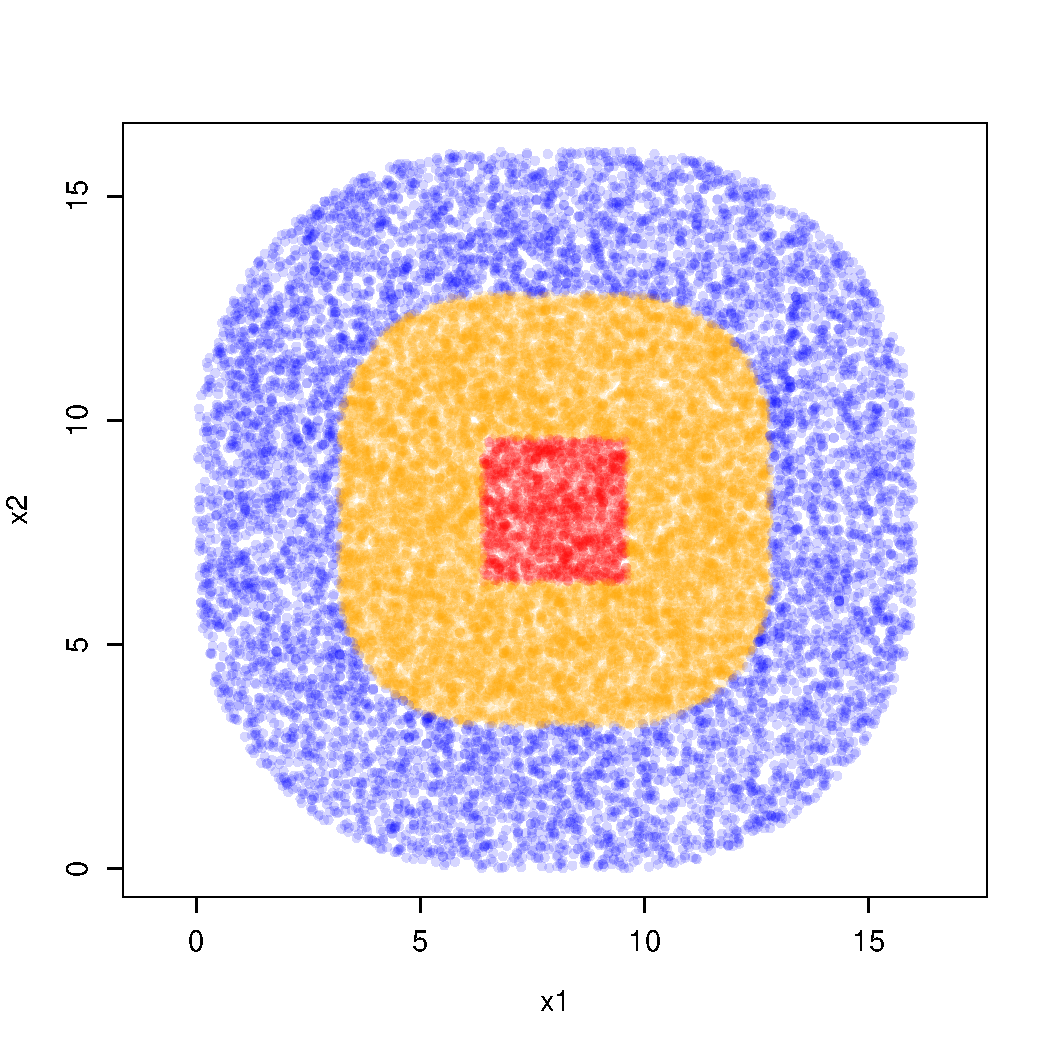
\includegraphics[width=0.32\textwidth]{example1plots/sample2}
  % \caption{}
  % \end{subfigure}
  % \begin{subfigure}{.33\linewidth}
  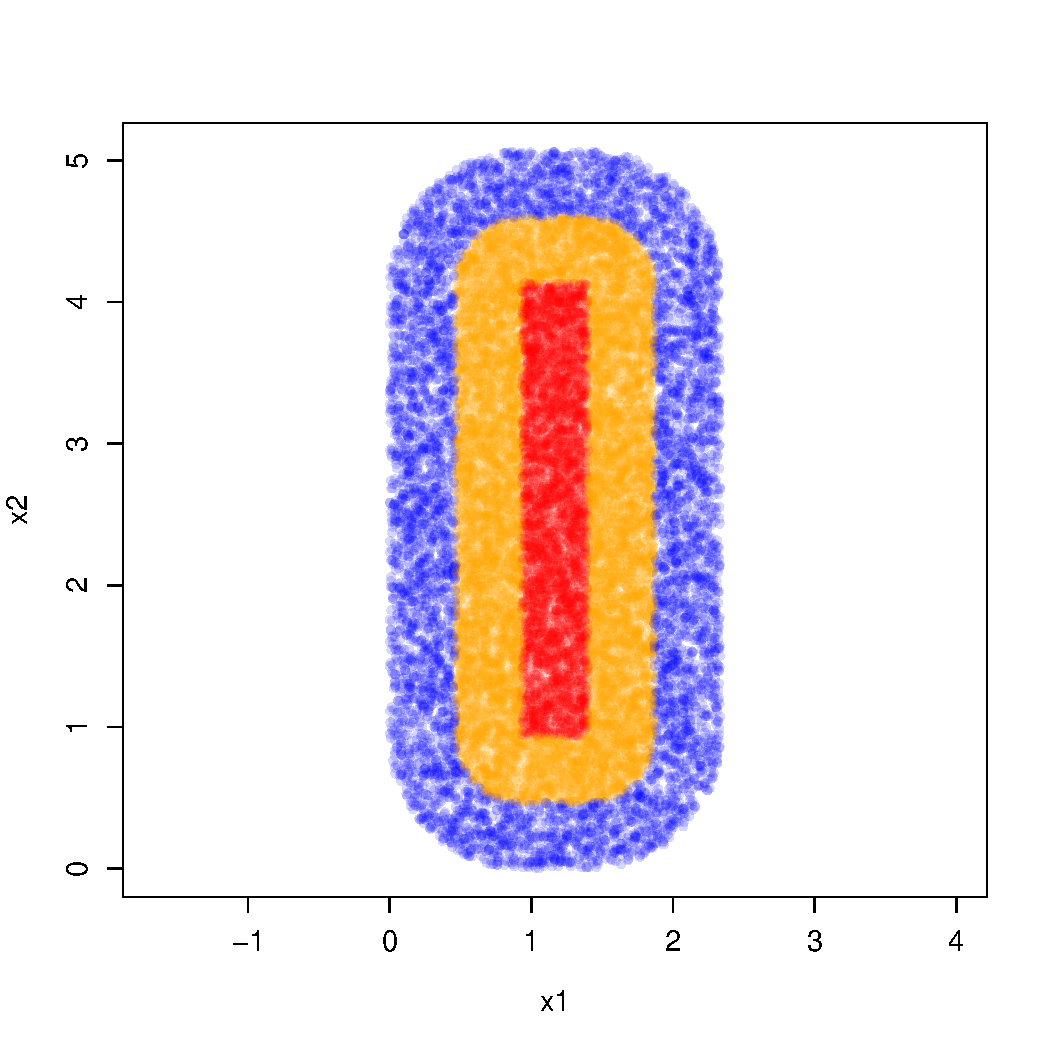
\includegraphics[width=0.32\textwidth]{example1plots/sample1}
  % \caption{}
  % \end{subfigure}
  % \begin{subfigure}{.33\linewidth}
  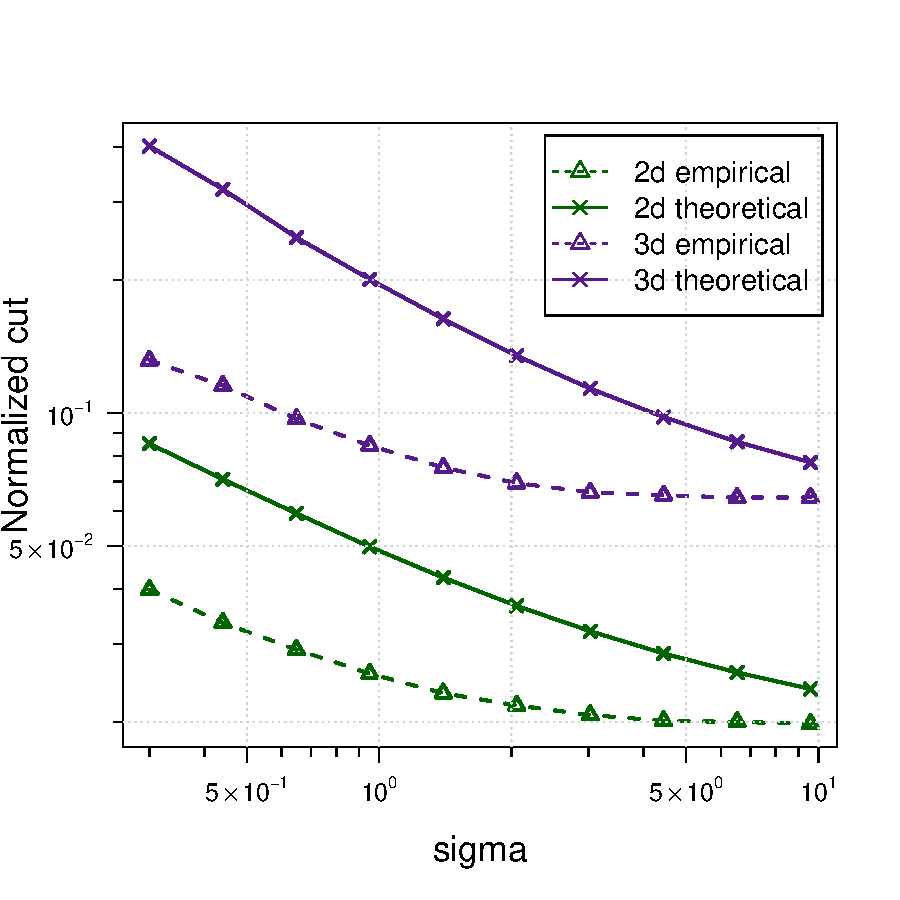
\includegraphics[width=0.32\textwidth]{example1plots/sigma_normalized_cut_plot}
  % \caption{}
  % \end{subfigure}
  
  % \begin{subfigure}{.33\linewidth}
  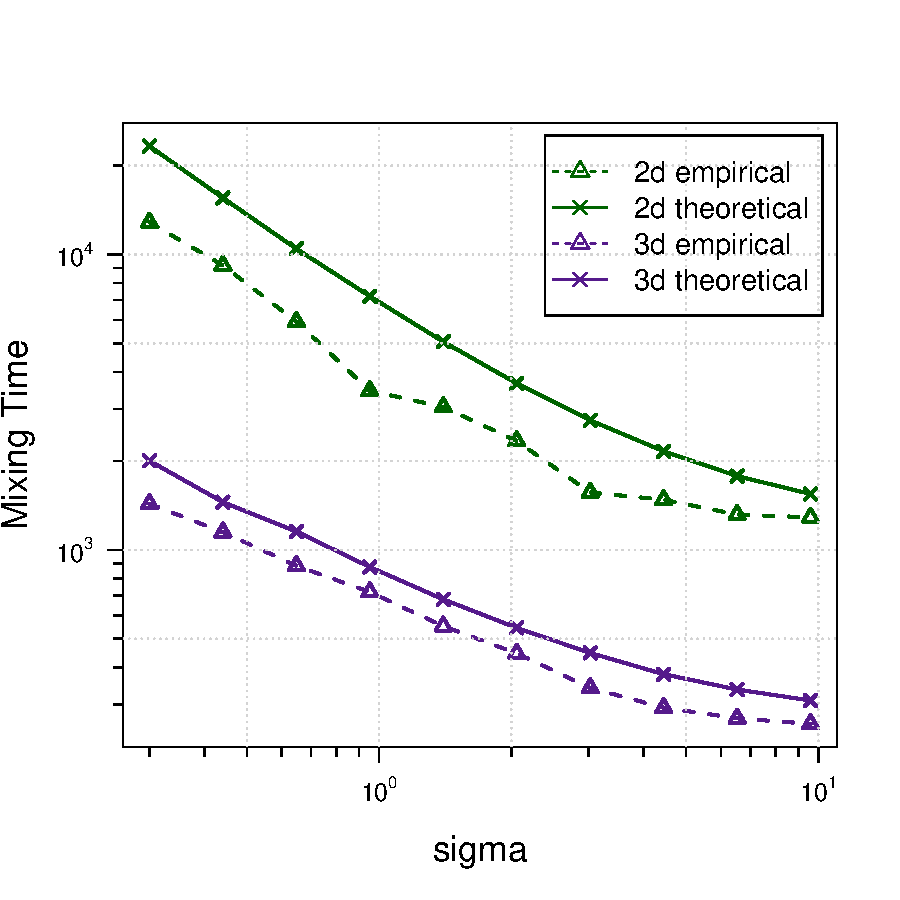
\includegraphics[width=0.32\textwidth]{example1plots/sigma_mixing_time_plot}
  % \caption{}
  % \end{subfigure}
  % \begin{subfigure}{.33\linewidth}
  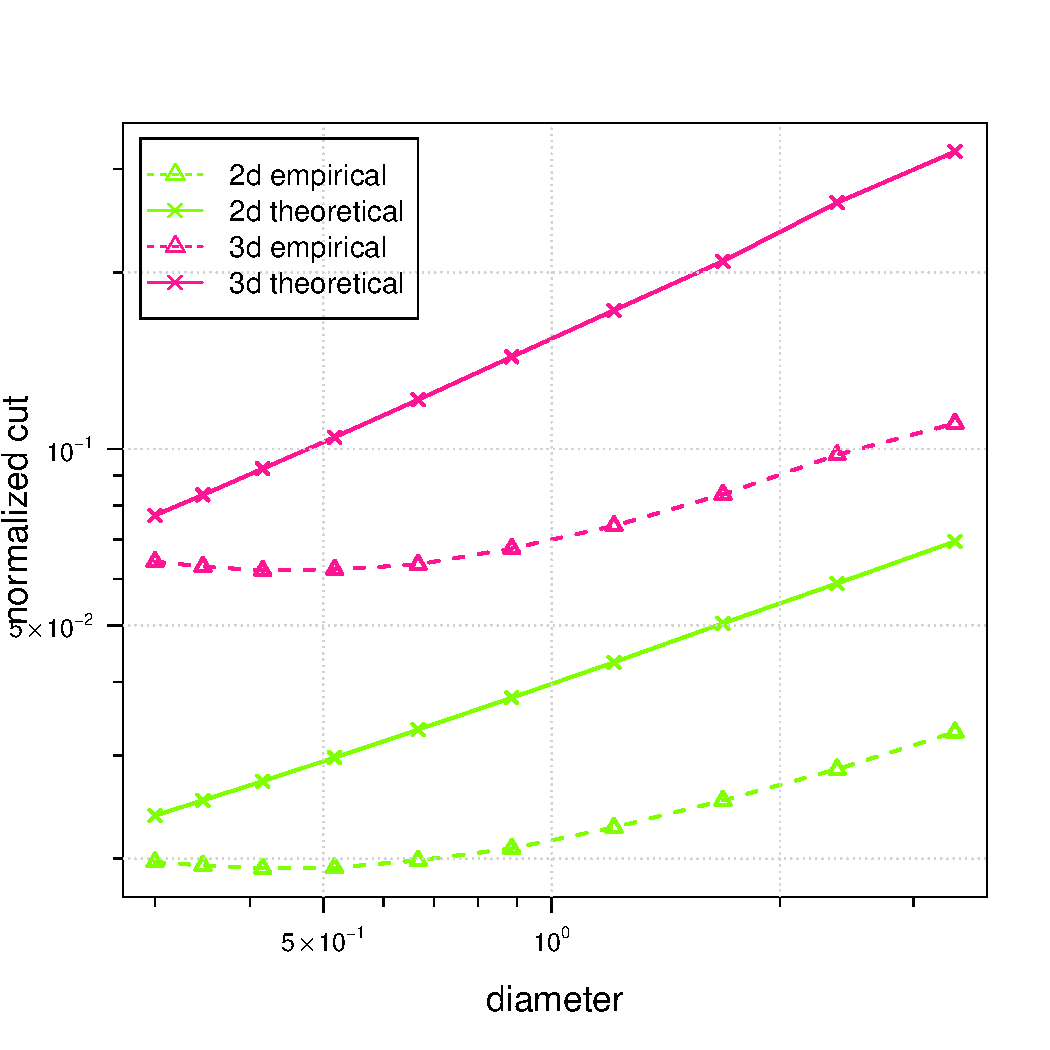
\includegraphics[width=0.32\textwidth]{example1plots/diameter_normalized_cut_plot}
  % \caption{}
  % \end{subfigure}
  % \begin{subfigure}{.33\linewidth}
  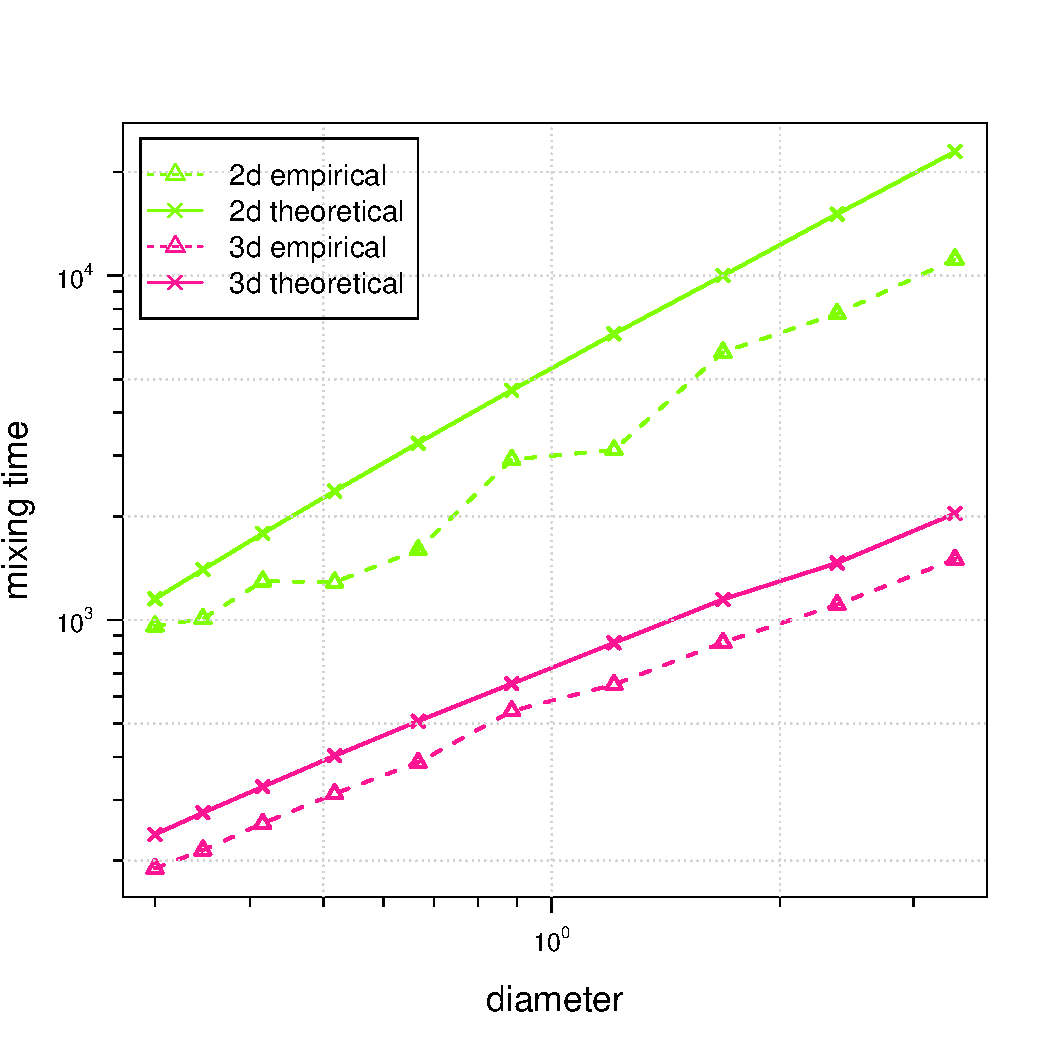
\includegraphics[width=0.32\textwidth]{example1plots/diameter_mixing_time_plot}
  % \caption{}
  % \end{subfigure}
  \caption{\it\small Top left and top middle: samples from a geometrically
    well- and poor-conditioned cluster. The points in $\Cset$ are colored in 
    red, points in $\Csig \setminus \Cset$ are colored in yellow, and the
    remaining points in blue. Other panels: empirical normalized cut and mixing
    time, as a function of $\sigma$ or $\rho$, versus their theoretical upper
    bounds.} 
  \label{fig:fig1}
%  \end{adjustbox}
\end{figure}

\paragraph{Validating theoretical bounds.}  We investigate the tightness of
Theorems \ref{thm: conductance_upper_bound} and \ref{thm:
  mixing_time_upper_bound} via simulation. Figure \ref{fig:fig1} compares our
upper bounds with the actual empirically-computed quantities \eqref{eqn:
  normalized_cut} and \eqref{eqn: mixing_time}, as we vary the diameter $\rho$
and thickness $\sigma$ of a cluster $\Cset$. The top left and top middle panels
display the resulting empirical clusters for two different values of
$\rho,\sigma$. 

The bottom left and bottom right panels assure that our mixing  
time upper bounds track closely the empirical mixing time, in both 2 and 3 
dimensions.\footnote{We rescaled all values of theoretical upper
  bounds by a constant, tto mask the effect of large universal constants
  in these bounds. Therefore only the comparison of slopes, rather than
  intercepts, is meaningful.} This provides empirical evidence that Theorem
\ref{thm: mixing_time_upper_bound} has the right dependency on both expansion
parameter $\sigma$ and diameter $\rho$. The story for the normalized cut panels
is less obvious. We remark that while, broadly speaking, the trends do not
appear to match, this gap between theory and empirical results seems largest
when $\sigma $ and $\rho$ are approximately equal. As the ratio $\rho/\sigma$
grows, the slopes of empirical and theoretical curves become more similar.

\paragraph{Empirical behavior of PPR.} In Figure \ref{fig:fig2}, to drive home
the main implications of Theorems \ref{thm: misclassification_rate} and
\ref{thm: consistent_recovery_of_density_clusters}, we show the
behavior of PPR, normalized cut, and the density clustering algorithm of
\citet{chaudhuri2010} on the well known ``two moons'' dataset (with added 2d 
Gaussian noise), considered a prototypical success story for spectral clustering
algorithms. The first column shows the empirical density clusters $\Cset[\Xbf]$
and $\Cset'[\Xbf]$ for a particular threshold $\lambda$ of the density function; the 
second column shows the cluster recovered by PPR; the third column shows the
global minimum normalized cut, computed according to the algorithm of
\citet{szlam2010}; and the last column shows a cut of the density cluster tree
estimator of \citet{chaudhuri2010}.  We can see the degrading ability of PPR to
recover density clusters as the two moons become less well-separated. Of 
particular interest is the fact that PPR fails to recover one of the moons even
when normalized cut still succeeds in doing so, supporting our claim from Remark
\ref{rmk: diameter}. Additionally, we note that the Chaudhuri-Dasgupta algorithm 
succeeds even when both PPR and normalized cut fail.  While our main message was
that PPR recovers geometrically well-conditioned density clusters, it would be  
interesting to establish that it \emph{only} recovers such clusters, a direction
for future work.   

\begin{figure}
  \centering
  % \begin{adjustbox}{minipage=\linewidth}
  %   \begin{subfigure}{.24\linewidth}
  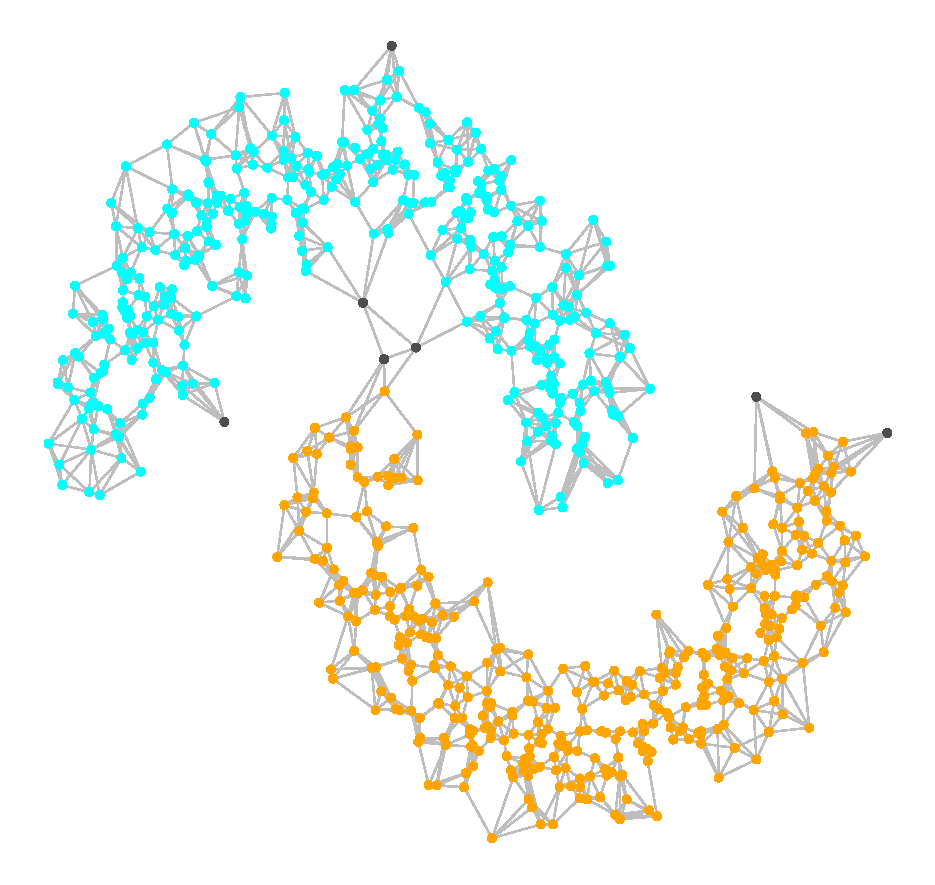
\includegraphics[width=0.24\textwidth,scale = .5]{example2plots/row1_true_density_cluster}
  % \caption{}
  % \end{subfigure}
  % \begin{subfigure}{.24\linewidth}
  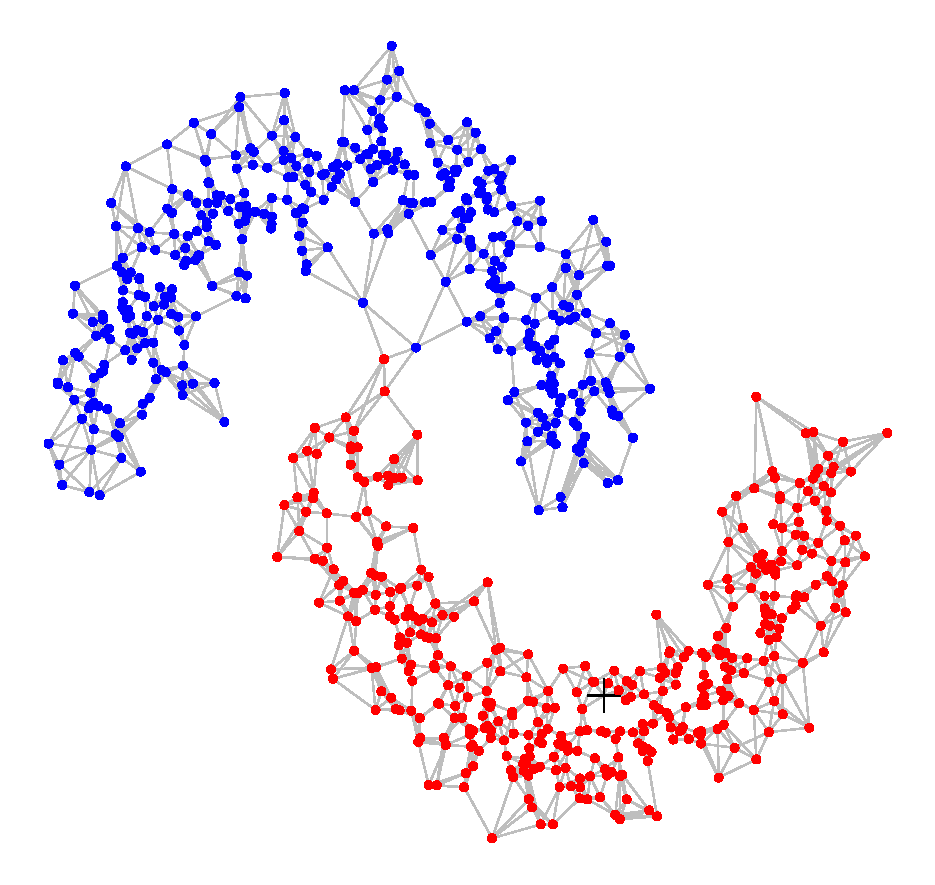
\includegraphics[width=0.24\textwidth]{example2plots/row1_ppr_cluster}
  % \caption{}
  % \end{subfigure}
  % \begin{subfigure}{.24\linewidth}
  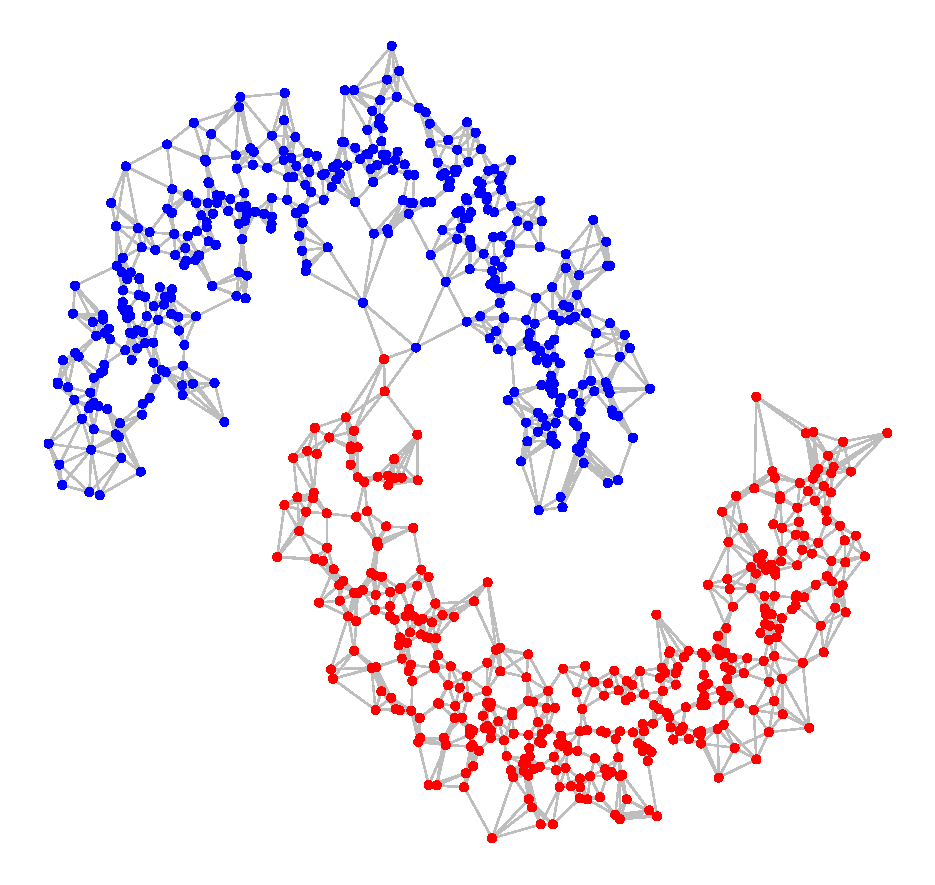
\includegraphics[width=0.24\textwidth]{example2plots/row1_conductance_cluster}
  % \caption{}
  % \end{subfigure}
  % \begin{subfigure}{.24\linewidth}
  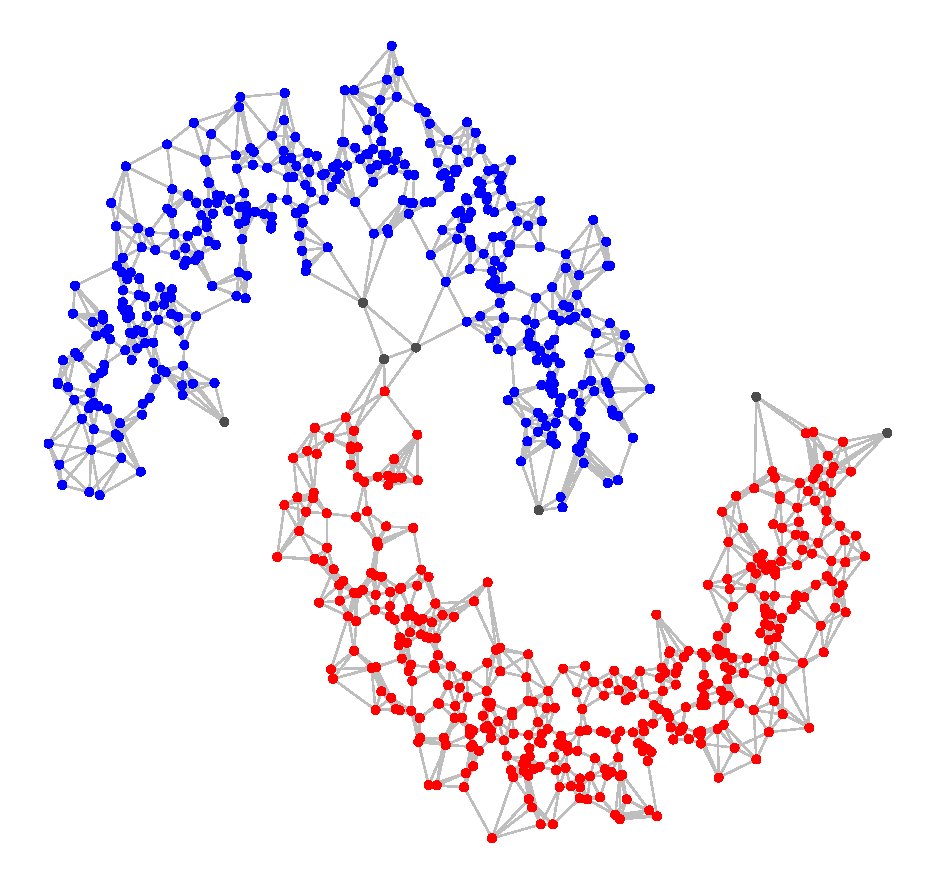
\includegraphics[width=0.24\textwidth]{example2plots/row1_density_cluster}
  % \caption{}
  % \end{subfigure}
  
  % \begin{subfigure}{.24\linewidth}
  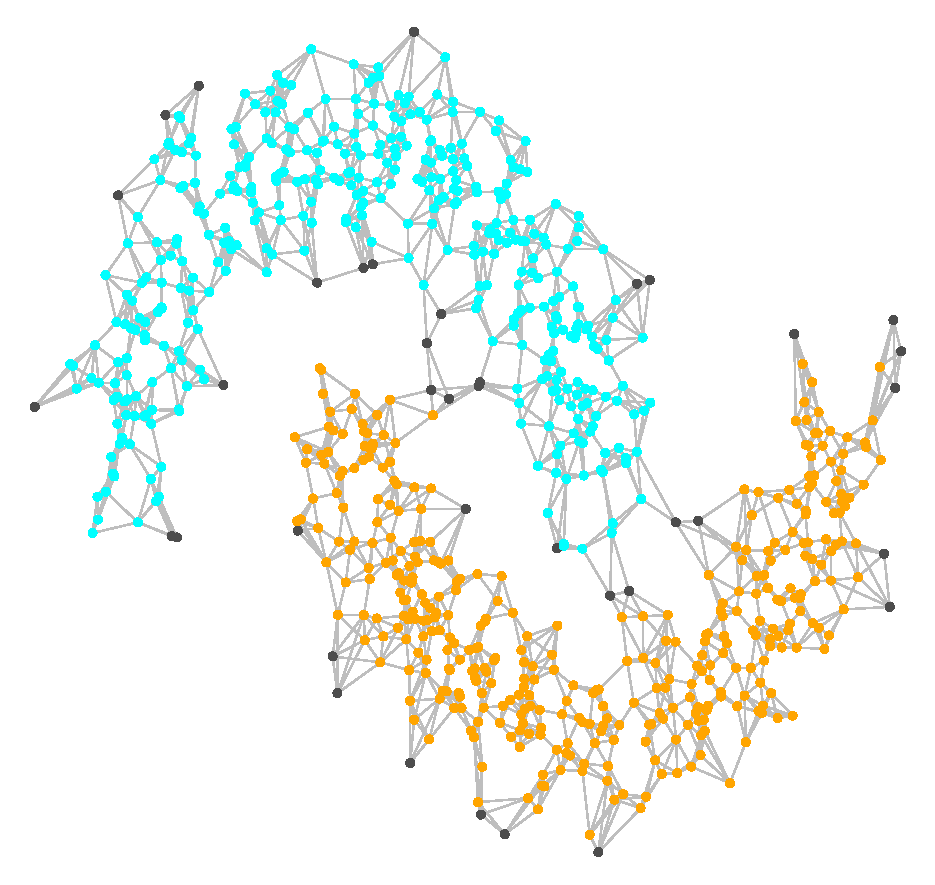
\includegraphics[width=0.24\textwidth]{example2plots/row2_true_density_cluster}
  % \caption{}
  % \end{subfigure}
  % \begin{subfigure}{.24\linewidth}
  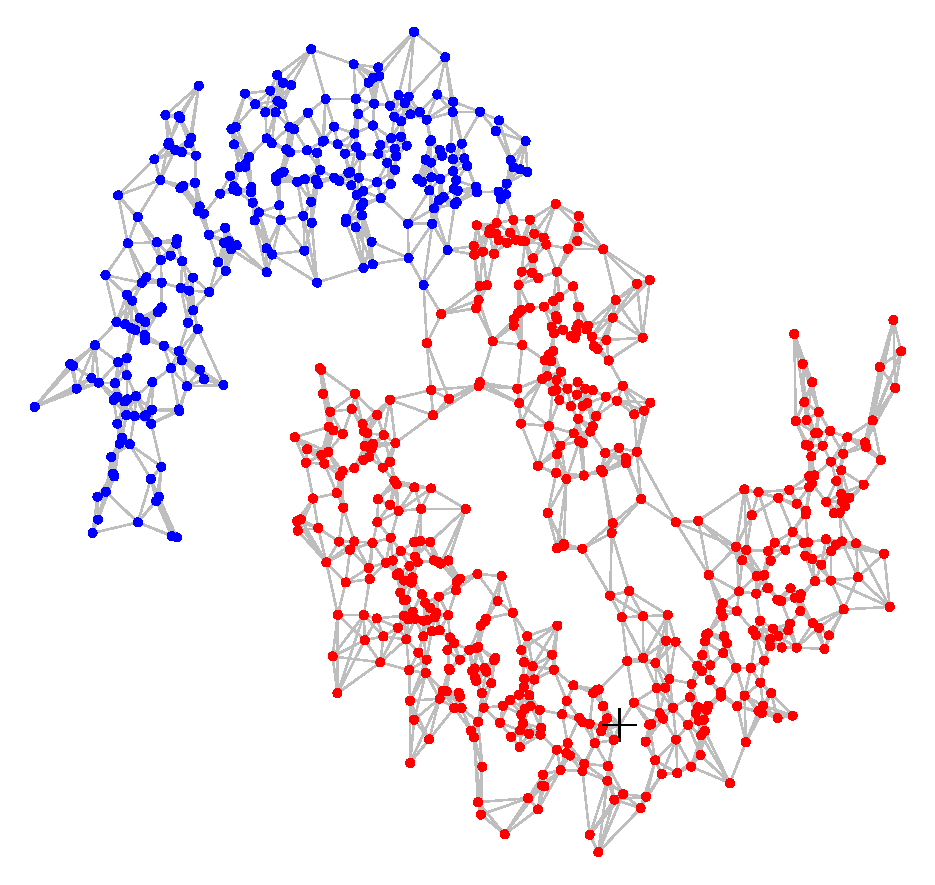
\includegraphics[width=0.24\textwidth]{example2plots/row2_ppr_cluster}
  % \caption{}
  % \end{subfigure}
  % \begin{subfigure}{.24\linewidth}
  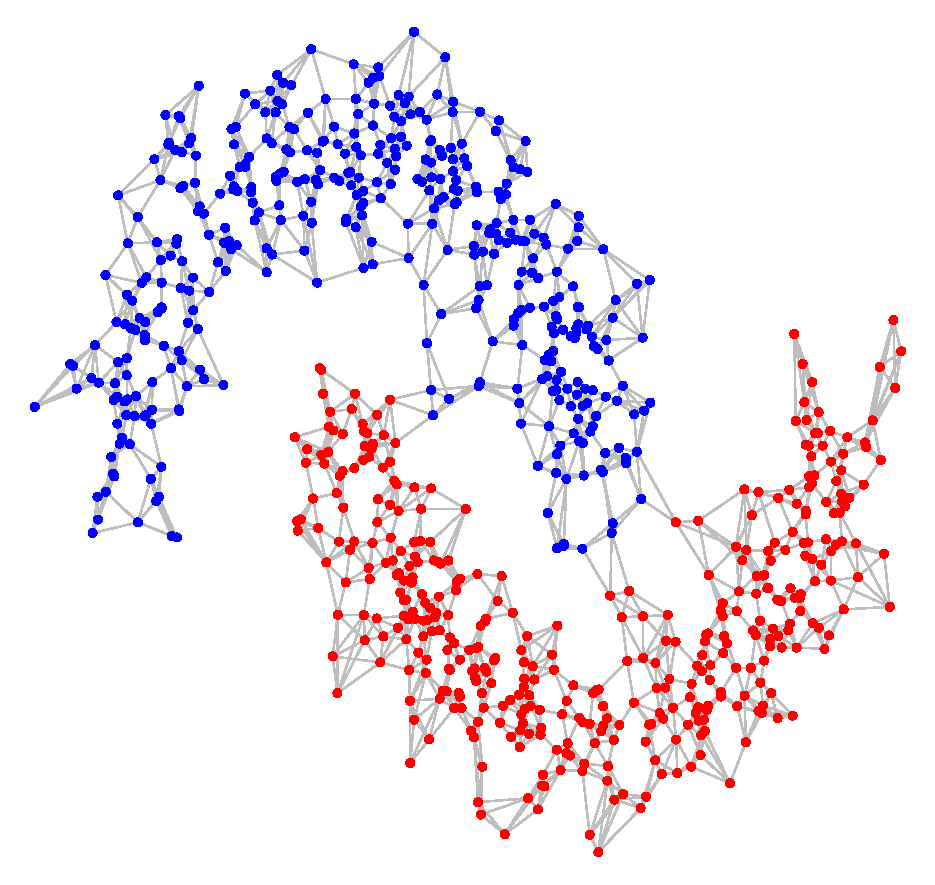
\includegraphics[width=0.24\textwidth]{example2plots/row2_conductance_cluster}
  % \caption{}
  % \end{subfigure}
  % \begin{subfigure}{.24\linewidth}
  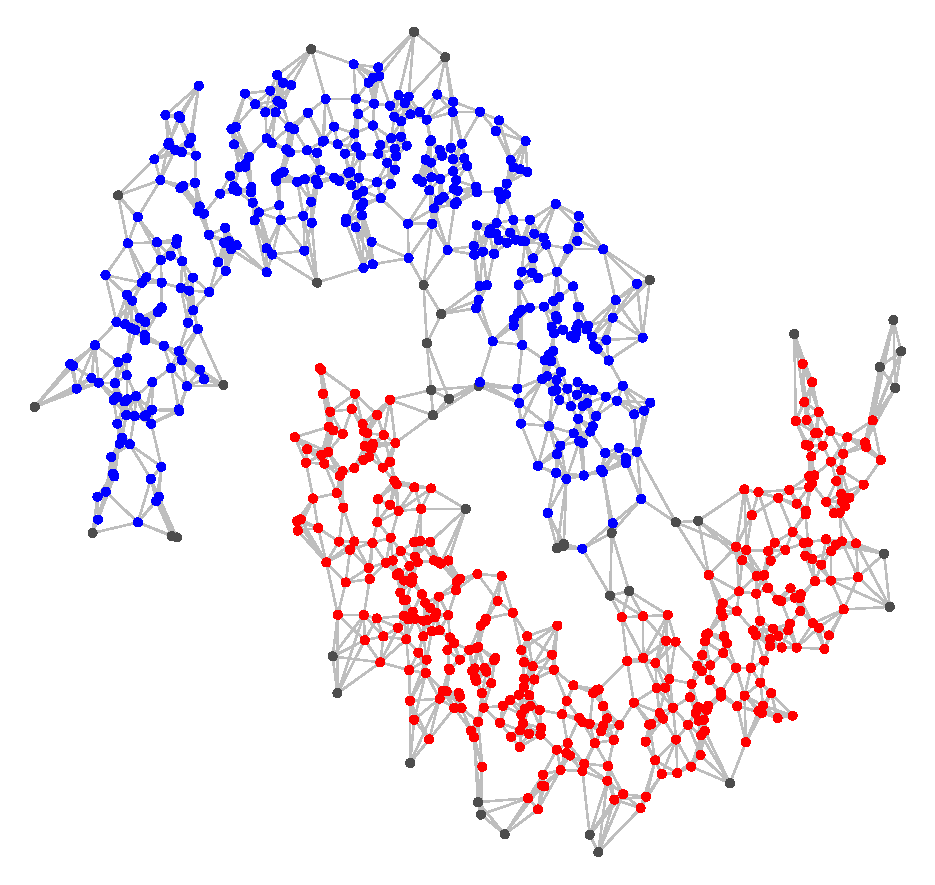
\includegraphics[width=0.24\textwidth]{example2plots/row2_density_cluster}
  % \caption{}
  % \end{subfigure}
  
  % \begin{subfigure}{.24\linewidth}
  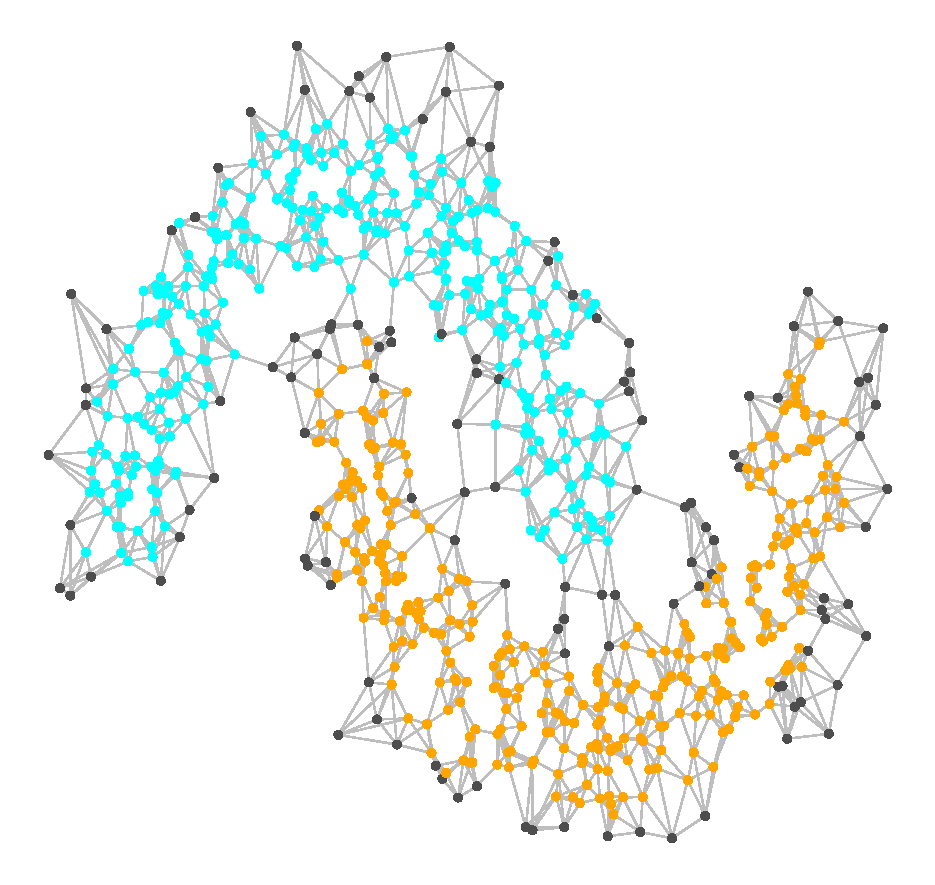
\includegraphics[width=0.24\textwidth]{example2plots/row3_true_density_cluster}
  % \caption{}
  % \end{subfigure}
  % \begin{subfigure}{.24\linewidth}
  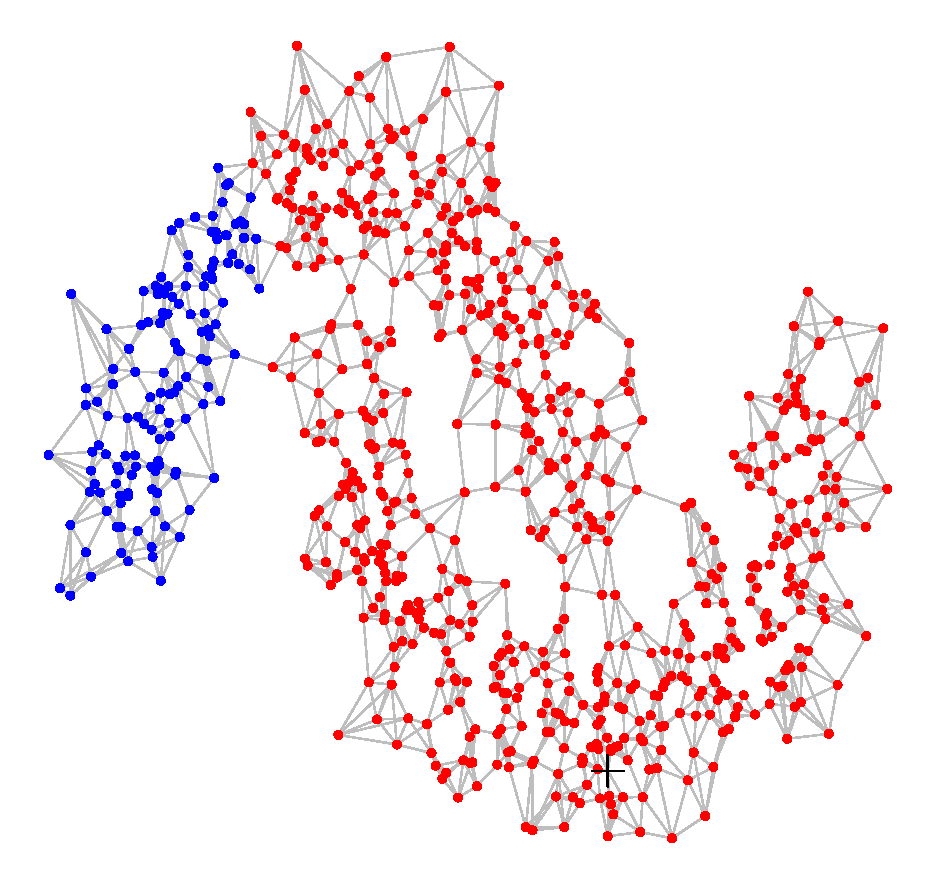
\includegraphics[width=0.24\textwidth]{example2plots/row3_ppr_cluster}
  % \caption{}
  % \end{subfigure}
  % \begin{subfigure}{.24\linewidth}
  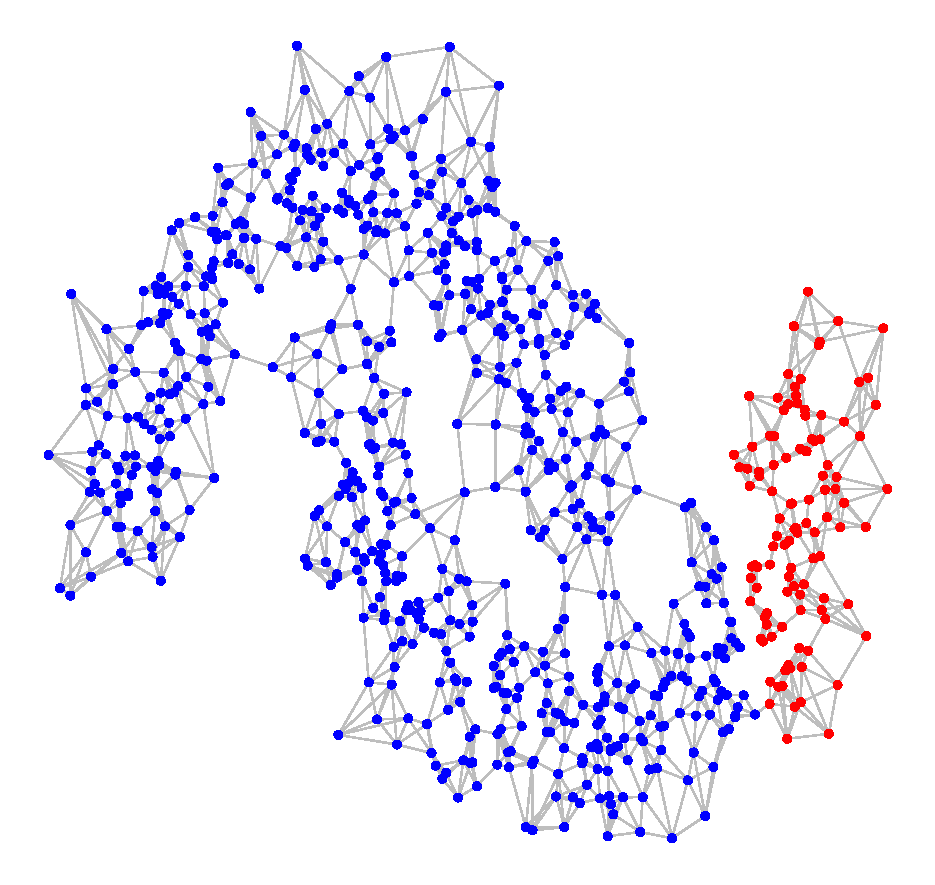
\includegraphics[width=0.24\textwidth]{example2plots/row3_conductance_cluster}
  % \caption{}
  % \end{subfigure}
  % \begin{subfigure}{.24\linewidth}
  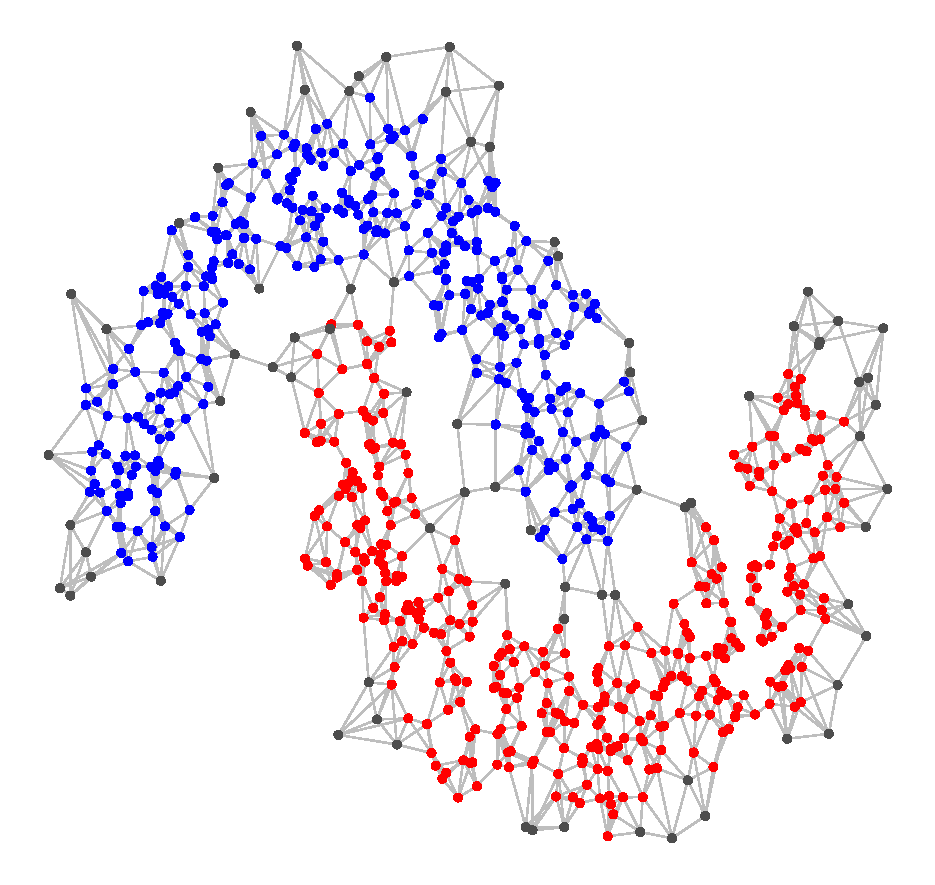
\includegraphics[width=0.24\textwidth]{example2plots/row3_density_cluster}
  % \caption{}
  % \end{subfigure}
  \caption{\it\small True density (column 1), PPR (column 2), normalized
    cut (column 3) and estimated density (column 4) clusters for 3 different 
    simulated data sets. Seed node for PPR denoted by a black cross.} 
  \label{fig:fig2}
  %\end{adjustbox}
\end{figure}

\section{Discussion}
\label{sec: discussion}

There are an almost limitless number of ways to define what the ``right''
clustering is. In this paper, we have considered one such notion---density upper
level sets---and have detailed a set of natural geometric criteria which, when 
appropriately satisfied, translate to provable bounds on estimation of the
cluster by PPR. We do not, however, provide theory to show that our geometric
conditions are required for successful recovery of a density level set. This
seems to be supported by our empirical results, and it remains a direction for 
future work.  

\section{Acknowledgements}
SB is grateful to Peter Bickel, Martin Wainwright and Larry Wasserman for helpful and inspiring conversations. This work was supported in part by the NSF grant DMS-1713003.

\appendix

%In this supplement, we present proofs and experimental details for the article ``Local Spectral Clustering of Density Upper Level Sets''.
\section{Proof of Theorem \ref{thm: conductance_upper_bound}}
\label{sec: proof_of_theorem_1}

For notational ease, we write
\begin{align*}
\cut_{n,r} = \cut(\Csig[\Xbf]; G_{n,r}), ~ \mu_K = \mathbb{E}(\cut_{n,r}), ~ p_K = \frac{\mu_K}{{n \choose 2}} \\
\vol_{n,r} = \vol(\Csig[\Xbf]; G_{n,r}), ~ \mu_V = \mathbb{E}(\vol_{n,r}), ~ p_V = \frac{\mu_V}{{n \choose 2}} \\
\vol_{n,r}^c = \vol(\Xbf \setminus \Csig[\Xbf]; G_{n,r}), ~ \mu_V^c = \mathbb{E}(\vol_{n,r}^c), ~ p_V^c = \frac{\mu_V^c}{{n \choose 2}}
\end{align*}
for the random variable, mean, and probability of cut size and volume, respectively.

With this notation in place, the goal of Theorem~\ref{thm: conductance_upper_bound} is roughly to show that, with probability at least $1 - \delta$, for a universal constant $c_1 > 0$ and for any $\epsilon > 0$, for a sufficiently large sample size $n$:
\begin{align*}
\Phi_{n,r}(\Csig[\Xbf]) := \frac{\cut_{n,r}}{\min\{\vol_{n,r}, \vol_{n,r}^c\}} \leq c_1 \frac{d}{\sigma}
    \frac{\lambda}{\lambda_{\sigma}} \frac{(\lambda_{\sigma} -
      c_0\frac{r^{\gamma}}{\gamma+1})}{\lambda_{\sigma}} + \epsilon.
\end{align*}

The proof of this theorem follows essentially from two technical Lemmas. 
The following Lemma relates the terms in the numerator and denominator of $\Phi_{n,r}(\Csig[\Xbf])$ to their expected values.
\begin{lemma}
	\label{lem: prob_bound_cutvol}
	For any $\delta \in (0,1]$,
	\begin{equation}
	\label{eqn: numerator_additive_bound}
	\frac{\cut_{n,r}}{{n \choose 2}} \leq p_K + \sqrt{\frac{\log(1/\delta)}{n}}, \\ 
	\frac{\vol_{n,r}}{{n \choose 2}} \geq p_V - \sqrt{\frac{\log(1/\delta)}{n}}, \\
	\frac{\vol_{n,r}^c}{{n \choose 2}} \geq p_V^c - \sqrt{\frac{\log(1/\delta)}{n}},
	\end{equation}
	each with probability at least $1 - \delta$. 
\end{lemma}
We note that as a consequence of~\ref{asmp: bounded_volume} we have that $p_V^c \geq p_V$, so it will suffice to lower bound $p_V$ (since a lower bound for $p_V^c$ follows).
The 
following result provides upper and lower bounds on the expected values $p_K$ and $p_V$ respectively:
\begin{lemma}
	\label{lem: expected_density_cut}\label{lem: expected_density_volume}
	Under the setup and conditions of Theorem \ref{thm: conductance_upper_bound}, and for any $0 < r \leq \sigma/2d$,
	\begin{align}
	p_K &\leq \frac{4 d \nu_d r^{d+1} \lambda}{\sigma} \left(\lambda_{\sigma} - c_0\frac{r^{\gamma}}{\gamma + 1}\right) \nu(\Csig), \label{eqn:claim_one} \\
	p_V &\geq \frac{12}{25} \lambda_{\sigma}^2 \nu_d r^d \nu(\Csig).\label{eqn:claim_two}
	\end{align}
\end{lemma}
%\begin{lemma}
%	\label{lem: expected_density_volume}
%	Under the setup and conditions of Theorem \ref{thm: conductance_upper_bound}, and for any $0 < r \leq \sigma/2d$,
%	\begin{equation*}
%	p_V \geq \frac{12}{25} \lambda_{\sigma}^2 \nu_d r^d \nu(\Csig).
%	\end{equation*}
%\end{lemma}



Taking these two technical lemmas as given we can now complete the proof of the theorem. 
We fix $\delta \in (0,1]$ and let $\delta' = \delta/3$. We rewrite
\begin{equation}
\label{eqn: conductance_representation_1}
\Phi_{n,r}(\Csig[\Xbf]) = \frac{p_K + \left(\frac{\cut_{n,r}}{{n \choose 2}} - p_K\right)}{p_V + \left(\frac{\min\set{\vol_{n,r}, \vol_{n,r}^c}}{{n \choose 2}} - p_V\right)}.
\end{equation}
By a union bound we see that all three bounds in \eqref{eqn: numerator_additive_bound} hold with probability at least $1 - \delta$. Along with (\ref{eqn: conductance_representation_1}) this yields the upper bound \sbcomment{Changed $\mathbf{X}$ to $X$}
\begin{equation*}
\Phi_{n,r}(\Csig[X]) \leq \frac{p_K + \Err_n}{p_V - \Err_n}
\end{equation*}
for $\Err_n = \sqrt{\frac{\log(1/\delta')}{n}}$.
Now, some straightforward algebraic manipulations yield,
\begin{align*}
\frac{p_K + \Err_n}{p_V - \Err_n} & = \frac{p_K}{p_V} \left(\frac{p_V}{p_V - \Err_n}\right) + \frac{\Err_n}{p_V - \Err_n} \\
& = \frac{p_K}{p_V} + \left(\frac{p_K}{p_V} + 1\right)\frac{\Err_n}{p_V - \Err_n} \\
& \leq \frac{p_K}{p_V} + 2 \frac{\Err_n}{p_V - \Err_n}.
\end{align*}

%The proof of Theorem \ref{thm: conductance_upper_bound} is more or less given by Lemmas \ref{lem: expected_density_cut}, \ref{lem: expected_density_volume}, and \ref{lem: prob_bound_cutvol}. All that remains is some algebra, which we take care of below.

\noindent Using Lemma \ref{lem: expected_density_cut}, we have
\begin{equation*}
\frac{p_K}{p_V} \leq \frac{100rd}{12\sigma} \frac{\lambda}{\lambda_{\sigma}} \frac{\left(\lambda_{\sigma} - c_0\frac{r^{\gamma}}{\gamma + 1}\right)}{\lambda_{\sigma}}.
\end{equation*}
Then, by the choice of sample size in \eqref{eqn: conductance_sample_complexity}, 
\begin{equation*}
n \geq \frac{(2 + \epsilon)^2 \log\left(\frac{3}{\delta}\right)}{\epsilon^2 p_V^2}
\end{equation*}
which implies $2 \frac{\Err_n}{p_V - \Err_n} \leq \epsilon$, and this yields the desired bound on $\Phi_{n,r}(\Csig[X])$. In order to complete the proof of
the theorem it remains to prove Lemmas~\ref{lem: prob_bound_cutvol} and~\ref{lem: expected_density_cut}.

\subsection{Proof of Lemma~\ref{lem: prob_bound_cutvol}}
We first note that we can write $\cut_{n,r}$ as a double sum,
	\begin{equation}
	\label{eqn: density_cut_expansion}
	\cut_{n,r} = \sum_{i = 1}^{n} \sum_{j \neq i} \1(x_i \not\in \Csig) \1(x_j \in \Csig) \1(\norm{x_i - x_j} \leq r),
	\end{equation}
	and similarly we can write $\vol_{n,r}$ as a sum of indicator functions,
	\begin{equation}
	\label{eqn: volume_expansion}
	\vol_{n,r} = \sum_{i = 1}^{n} \sum_{j \neq i} \1(x_i \in \Csig) \1(x_j \in B(x_i, r)).
	\end{equation}
From this we see that $\cut_{n,r}$ and $\vol_{n,r}$, properly scaled, can be expressed as order-$2$ $U$-statistics,
	\begin{equation*}
	\frac{\cut_{n,r}}{{n \choose 2}} = \frac{1}{{n \choose 2}} \sum_{1 \leq i < j \leq n} \phi_K(x_i, x_j),~~ \frac{\vol_{n,r}}{{n \choose 2}} = \frac{1}{{n \choose 2}} \sum_{1 \leq i < j \leq n} \phi_V(x_i, x_j)
	\end{equation*}
	with kernels
	\begin{align*}
	\phi_K(x_i,x_j) & = \1(x_i \in \Csig, x_j \not\in \Csig, \norm{x_i - x_j} \leq r) + \1(x_j \in \Csig, x_i \not\in \Csig, \norm{x_i - x_j} \leq r) \\
	\phi_V(x_i,x_j) & = \1(x_i \in \Csig, \norm{x_i - x_j} \leq r) + \1(x_j \in \Csig, \norm{x_i - x_j} \leq r). 
	\end{align*}
	Similarly,
	\begin{equation*}
	\frac{\vol_{n,r}^c}{{n \choose 2}} = \frac{1}{{n \choose 2}} \sum_{1 \leq i < j \leq n} \phi_{V^c}(x_i, x_j)
	\end{equation*}
	with kernel,
	\begin{equation*}
	\phi_{V^c}(x_i,x_j) = \1(x_i \not\in \Csig, \norm{x_i - x_j} \leq r) + \1(x_j \not\in \Csig, \norm{x_i - x_j} \leq r). 
	\end{equation*}
	Appealing to a standard concentration inequality for U-statistics (see Lemma \ref{lem: bounded_difference}) we therefore have
	\begin{equation*}
	\frac{\cut_{n,r}}{{n \choose 2}} \leq p_K + \sqrt{\frac{\log(1/\delta)}{n}},~  \frac{\vol_{n,r}}{{n \choose 2}} \geq p_V - \sqrt{\frac{\log(1/\delta)}{n}}, ~ \frac{\vol_{n,r}^c}{{n \choose 2}} \geq p_V^c - \sqrt{\frac{\log(1/\delta)}{n}}
	\end{equation*}
	each with probability at least $1 - \delta$. 
	%The claim follows in light of \ref{asmp: bounded_volume}, which implies $p_V^c \geq p_V$. 


\subsection{Proof of Lemma~\ref{lem: expected_density_cut}}
We write $\Pbb(\Aset) = \int_{\Aset} f(x) dx$ for measurable $\Aset \subseteq \Rd$.
We 
let $\Csigr := \set{x: 0 < \dist(x, \Csig) < r}$, where $\Csig$ is as in Theorem \ref{thm: conductance_upper_bound}. 
Our goal will be to upper bound $p_K$ by a term that depends on the probability mass $\Pbb(\Csigr)$, 
and the bulk of our technical effort will be devoted to showing the following upper bound on $\Pbb(\Csigr)$:
%Lemma \ref{lem: expected_number_boundary_points} involves the bulk of the technical effort required to prove Theorem \ref{thm: conductance_upper_bound}; it will be necessary to bound the expected cut size of $\Csig[\Xbf]$ in $G_{n,r}$. 
\begin{lemma}
	\label{lem: expected_number_boundary_points}
	Under the conditions of Theorem \ref{thm: conductance_upper_bound}, and for any $0 < r \leq \sigma/2d$,
	\begin{equation*}
	\Pbb(\Csigr) \leq \frac{2dr}{\sigma} \left(\lambda_{\sigma} - c_0\frac{r^{\gamma}}{\gamma + 1}\right) \nu(\Csig)
	\end{equation*}	
\end{lemma}
\noindent Define the \emph{uniform local conductance} $\ell_{\nu,r}(u)$ to be
\begin{equation*}
\ell_{\nu,r}(u) = \nu\bigl(\Csig \cap B(u,r)\bigr).
\end{equation*}
In order to lower bound $p_V$ we will show the following lower bound on the uniform local conductance:
\begin{lemma}
	\label{lem: local_conductance}
	Let $u \in \Csig$. Then, for any $0 < r \leq \frac{\sigma}{2\sqrt{d}}$,
	\begin{equation*}
	\ell_{\nu,r}(u) \geq \frac{6}{25} \nu_d r^d.
	\end{equation*}
\end{lemma}
Taking these two results as given we can now prove each of the two claims~\eqref{eqn:claim_one} and~\eqref{eqn:claim_two} in turn.
\paragraph{Proof of Claim~\eqref{eqn:claim_one}: } Recalling,~\eqref{eqn: density_cut_expansion} 
	and by the linearity of expectations, we obtain
	\begin{equation*}
	p_K = \frac{\mu_K}{{n \choose 2}} = 2 \cdot \Pbb(x_i \not\in \Csig, x_j \in \Csig, \norm{x_i - x_j} \leq r). \tag{for each $i,j$, $i \neq j$}
	\end{equation*}
	Writing this with respect to the density function $f$, we have
	\begin{align*}
	p_K & = 2 \int_{\Rd \setminus \Csig} f(x) \Pbb\bigl(B(x,r) \cap \Csig\bigr) \dx \\
	& = 2 \int_{\Csigr} f(x) \Pbb\bigl(B(x,r) \cap \Csig\bigr) \dx \\
	& \leq 2 \nu_d r^d \lambda  \int_{\Csigr} f(x) \dx = 2 \nu_d r^d \lambda \Pbb(\Csigr).
	\end{align*}
	where the inequality follows from \ref{asmp: cluster_separation}, which implies $f(x) \leq \lambda$ for $x \in \Csig \setminus \Cset$. Then, upper bounding the integral using \sbcomment{I changed the Lemma referenced here. I think it was wrong before} Lemma \ref{lem: expected_number_boundary_points} gives the final result.


%\subsection{Proof of Lemma~\ref{Z}}
\paragraph{Proof of Claim~\eqref{eqn:claim_two}: } Recalling,~\eqref{eqn: volume_expansion}
%The proof will proceed similarly to Lemma \ref{lem: expected_density_cut}. 
	and by the linearity of expectation we obtain
	\begin{equation*}
	p_V = \frac{\mu_V}{{n \choose 2}} = 2 \cdot \Pbb(x_i \in \Csig, x_j \in B(x_i,r)). \tag{for any $i,j$, $i \neq j$. }
	\end{equation*}
	Writing this with respect to the density function $f$, we have
	\begin{align*}
	p_V & = 2 \int_{\Csig} f(x) \Pbb(B(x,r)) \dx \\
	& \geq 2 \int_{\Csig} f(x) \Pbb(B(x,r) \cap \Csig) \dx
	\end{align*}
	whence the claim then follows by Lemma \ref{lem: local_conductance}.
It remains to prove Lemmas~\ref{lem: expected_number_boundary_points} and~\ref{lem: local_conductance}, and we turn our attention to this next.
\subsection{Proof of Lemma~\ref{lem: expected_number_boundary_points}}
The proof of this Lemma relies on certain volume estimates whose statement and proof we defer to Appendix~\ref{sec: volume_estimates}.
	We partition $\Csigr$ into slices based on distance from $\Csig$ as follows: for $k \in \N$,
	\begin{equation*}
	\mathcal{T}_{i,k} = \set{x \in \Csigr: t_{i,k} < \frac{\dist(x, \Csig)}{r} \leq t_{i+1,k}}, ~~ \Csigr = \bigcup_{i = 0}^{k-1} \mathcal{T}_{i,k},
	\end{equation*}
	\sbcomment{Changed $t_i$ to $t_{i,k}$.}
	where $t_{i,k} = i/k$ for $i = 0, \ldots, k - 1$. As a result, for any $k \in \mathbb{N}$,
	\begin{equation}
	\label{eqn: partition_ub}
	\Pbb(\Csigr) = \int_{\Csigr} f(x) \dx = \sum_{i = 0}^{k-1} \int_{\mathcal{T}_{i,k}} f(x) \dx \leq \sum_{i = 0}^{k-1} \nu(\mathcal{T}_{i,k}) \max_{x \in \mathcal{T}_{i,k}} f(x).
	\end{equation}
	Assumptions~\ref{asmp: bounded_density} and \ref{asmp: low_noise_density} imply the upper bound
	\begin{equation*}
	\max_{x \in \mathcal{T}_{i,k}} f(x) \leq \lambda_{\sigma} - c_0(rt_{i,k})^{\gamma},
	\end{equation*}
	and writing
	\begin{equation*}
	\nu(\mathcal{T}_{i,k}) = \nu(\Csig + rt_{i+1,k}B) - \nu(\Csig + rt_{i,k}B) =: \nu_{i+1,k} - \nu_{i,k},
	\end{equation*}
	we have
	\begin{align}
	\label{eqn: telescoping_sum}
	\sum_{i = 0}^{k-1} \nu(\mathcal{T}_{i,k}) \max_{x \in \mathcal{T}_{i,k}} f(x) & \leq \sum_{i = 0}^{k-1} \biggl\{ \nu_{i+1,k} - \nu_{i,k} \biggr\} \biggl( \lambda_{\sigma} - c_0(rt_{i,k})^{\gamma} \biggr) \nonumber \\
	& = \underbrace{\sum_{i = 1}^{k} 
	\nu_{i,k} \biggl( \left[\lambda_{\sigma} - c_0(rt_{i-1,k})^{\gamma}\right] -  \left[\lambda_{\sigma} - c_0(rt_{i,k})^{\gamma}\right]\biggr)}_{:= \Sigma_k} + \underbrace{\biggl(\nu_{k,k}\left[\lambda_{\sigma} - c_0r^{\gamma}\right] - \nu_{1,k}\lambda_{\sigma} \biggr)}_{:= \xi}
	\end{align}
	\sbcomment{I changed the braces above -- I think they were incorrect earlier} where the second equality comes from rearranging terms in the sum.
	
	% AJG 5/14/19: This argument makes sense, correct?
	We first consider the term $\Sigma_k$. $\Cset$ has finite diameter by Assumption~\ref{asmp: bounded_density}, as otherwise $\int_{\Csig} f(x) dx = \infty$. Letting $\overline{\Cset}$ be the closure of $\Cset$, we observe that $\overline{\Csig} = \overline{\Cset} + \sigma B$, and moreover for any $\delta > 0$, $\nu(\overline{\Csig} + \delta B) = \nu(\Csig + \delta B)$ (as the boundary $\partial(\Csig + \delta B)$ is Lipschitz and therefore has measure zero). As a result, for each $t_{i,k}, i = 1, \ldots,k$ we may apply Lemma \ref{lem: expansion_volume} to $\overline{\Cset}$ and obtain
	\begin{equation}
	\label{eqn: slice_volume_bound}
	\nu_{i,k} = \nu(\Csig + rt_{i,k}B) \leq \nu(\Csig)\left(1 + \frac{rt_{i,k}}{\sigma}\right)^d
	\end{equation}
	which in turn gives
	\begin{align}
	\Sigma_k & \leq c_0\nu(\Csig) r^\gamma \sum_{i = 1}^{k} \left(1 + \frac{ rt_{i,k}}{\sigma}\right)^d \biggl( (t_{i,k})^{\gamma} - (t_{i-1,k})^{\gamma}\biggr) \nonumber \\
	& = c_0\nu(\Csig) r^\gamma \sum_{i = 1}^{k} \left(1 + \frac{ru_{i,k}^{1/\gamma}}{\sigma}\right)^d ( u_{i,k} - u_{i,k-1}).~~~~~~~~~~~~~~ (\text{substituting}~u_{i,k} := t_{i,k}^{\gamma}) \label{eqn: Sigmak_riemann_sum}
	\end{align}
	The expression in~\eqref{eqn: Sigmak_riemann_sum} is a Riemann sum, and taking the limit as $k \to \infty$ we obtain
	\begin{align}
	\lim_{k \to \infty} c_0\nu(\Csig) r^\gamma \sum_{i = 1}^{k} \left(1 + \frac{ru_{i,k}^{1/\gamma}}{\sigma}\right)^d ( u_{i,k} - u_{i,k-1}) & = c_0\nu(\Csig) r^\gamma \int_{0}^{1} \left(1 + \frac{r u^{1/\gamma}}{\sigma}\right)^{d} du \nonumber \\
	& \overset{\text{(i)}}{\leq} c_0\nu(\Csig) r^\gamma \int_{0}^{1} \left(1 + \frac{2 d r u^{1/\gamma}}{\sigma}\right) du \nonumber \\
	& = c_0\nu(\Csig) r^\gamma \left(1 + \gamma \frac{2 d r}{(\gamma + 1)\sigma}\right). \label{eqn: Sigmak_integral}
	\end{align}
	where $\text{(i)}$ follows from the upper bound in Lemma \ref{lem: Taylor_series} in light of the fact $r \leq \sigma / 2d$. 
	
	An upper bound on $\xi$ follows from largely the same logic, although it does not involve integration:
	\begin{align}
	\xi & \overset{\text{(ii)}}{\leq} \nu(\Csig) \biggl\{ \left(1 + \frac{ r}{\sigma}\right)^d(\lambda_{\sigma} - c_0r^{\gamma}) - \lambda_{\sigma} \biggr\} \nonumber \\
	& \overset{\text{(iii)}}{\leq} \nu(\Csig) \biggl\{ \left(1 + \frac{2d r}{\sigma}\right)(\lambda_{\sigma} - c_0r^{\gamma}) - \lambda_{\sigma} \biggr\} = \nu(\Csig) \biggl\{ \frac{2dr}{\sigma}(\lambda_{\sigma} - c_0r^{\gamma}) - c_0 r^{\gamma} \biggr\}. \label{eqn: xi_ub}
	\end{align}
	where $\text{(ii)}$ follows from \eqref{eqn: slice_volume_bound}, and $\text{(iii)}$ from Lemma \ref{lem: Taylor_series}. As the bounds in \eqref{eqn: partition_ub} and \eqref{eqn: telescoping_sum} hold for all $k$, these along with \eqref{eqn: Sigmak_integral} and \eqref{eqn: xi_ub} imply the desired result.



%\subsection{Proof of Lemma~\ref{lem: expected_number_boundary_points}}



\subsection{Proof of Lemma~\ref{lem: local_conductance}}
The proof of this result relies on estimates of the volume of spherical caps which we defer to Appendix~\ref{sec:caps}.
	Since $u \in \Csig$ there exists $x \in \Cset$ such that $u \in B(x, \sigma)$, and as $B(x,\sigma) \subseteq \Csig$,
	\begin{equation*}
	\nu\bigl(B(u, r) \cap B(x, \sigma)\bigr) \leq \nu\bigl(B(u, r) \cap \Csig \bigr)
	\end{equation*}
	Without loss of generality, let $\norm{u - x} = \sigma$; it is not hard to see that if $\norm{u - x} < \sigma$, the volume of the overlap will only grow. Then, since $\norm{u  - x} = \sigma$, $B(u, r) \cap B(x, \sigma)$ contains a spherical cap of radius $r$ and height
	\begin{equation*}
	h = r - r^2/2\sigma = r \left( 1 - \frac{r}{2 \sigma} \right)
	\end{equation*}	
	which by Lemma \ref{lem: volume_of_spherical_cap} has volume
	\begin{equation*}
	\nu_{\text{cap}} = \frac{1}{2} \nu_d r^d I_{1 - \alpha}\left( \frac{d + 1}{2}  ,\frac{1}{2}\right)
	\end{equation*}
	with $\alpha = 1 - \frac{2rh - h^2}{r^2} = \frac{r^2}{4 \sigma^2} \leq \frac{1}{16d}$. 
	By Lemmas \ref{lem: beta_integral} (applied with $t = 1$) and \ref{lem: beta_function},
	\begin{align*}
	I_{1 - \alpha}\left( \frac{d + 1}{2}  ,\frac{1}{2}\right) & \geq 1 - \frac{\Gamma\bigl(\frac{d}{2}+ 1\bigr)}{\Gamma\bigl(\frac{d + 1}{2}\bigr) \Gamma\bigl(\frac{1}{2}\bigr)} \frac{3}{4\sqrt{d}} \\
	& \geq 1 - \frac{3}{4}\sqrt{\frac{d+2}{\pi d}} \geq 1 - \frac{3}{4}\sqrt{\frac{3}{2 \pi}}.
	\end{align*}


\subsection{Volume Estimates}
\label{sec: volume_estimates}
%\section{Proofs}
%
%Subsections \ref{sec: volume_estimates} - \ref{sec: proof_of_theorem_1} detail the proof for Theorem \ref{thm: conductance_upper_bound}. In subsections \ref{sec: mixing_time_on_graphs} and \ref{sec: proof_of_proposition_tv_mixing_time}, we establish some results regarding mixing time over general graphs. The proof of Theorem \ref{thm: mixing_time_upper_bound} is then provided in subsections \ref{sec: population_conductance_function} - \ref{sec: proof_of_theorem_mixing_time}. Section~\ref{sec: concentration} gives some general concentration results we use throughout, before we finish with the proofs of Theorems \ref{thm: misclassification_rate} and \ref{thm: consistent_recovery_of_density_clusters}, and the statement and proof of our results regarding the a\pprspace vector (Corollary \ref{cor: appr}), in subsections \ref{sec: proof_of_misclassification_rate} - \ref{sec: linalg}.

%\subsection{Volume estimates}


We begin by recalling some notation. We let $\Aset \subseteq \Reals^d$, and for $\sigma \geq 0$, write $\sigma B := B(0,\sigma) = \set{x \in \Rd: \norm{x} \leq \sigma}$ for the closed ball of radius $\sigma$ centered at the origin (and let $B^{\circ}(0,\sigma)$ denote the corresponding open ball). Let $\Asig = \Aset + \sigma B$ be the direct sum of $\Aset$ and $\sigma B$, $\Asig = \set{z = x + y: x \in \Aset, y \in \sigma B}$. Recall that we use $\nu$ for Lebesgue measure, and $\nu_d = \nu(B)$ for $B = (0,1)$. 

Lemma \ref{lem: expansion_volume} provides a bound on the ratio $\nu(\Csig + r B) / \nu(\Csig)$, an important intermediate quantity in bounding the ratio $\cut(\Csig[\Xbf]; G_{n,r})/\vol(\Csig[\Xbf]; G_{n,r})$. 

\begin{lemma}
	\label{lem: expansion_volume}
	If $\Aset$ is closed and bounded, then for any $\delta > 0$,
	\begin{equation}
	\label{eqn: expansion_volume}
	\nu(\Asig + \delta B) \leq \left(1 + \frac{\delta}{\sigma}\right)^d \nu(\Asig).
	\end{equation}
\end{lemma}
\begin{proof}
	We will show that for any $\epsilon > 0$, 
	\begin{equation}
	\label{eqn: ratio_of_volume}
	\frac{\nu(\Asig + \delta B)}{\nu(\Asig)} \leq \frac{(\sigma + \delta + \epsilon)^d}{\sigma^d}
	\end{equation}
	Taking the limit as $\epsilon \to 0$ results in \eqref{eqn: expansion_volume}.
	
	
	Fix $\epsilon > 0$. Our first goal is to find a finite collection $x_1, \ldots, x_N \in \Rd$ (where $N$ is a finite number that may implicitly depend on $\epsilon$) such that
	\begin{equation*}
	\bigcup_{i = 1}^{N} B(x_i, \sigma) \subseteq \Asig \subset \bigcup_{i = 1}^{N} B(x_i, \sigma + \epsilon).
	\end{equation*}
	Note that $\Asig$ is the direct sum of two compact sets, and is therefore itself compact. Moreover, for any $\epsilon > 0$,
	\begin{equation*}
	\Asig \subset \bigcup_{x \in \Aset} B^{\circ}(x,\sigma + \epsilon)
	\end{equation*}
	so by compactness there exists a finite subcover $x_1, \ldots,x_N \in \Aset$ such that
	\begin{equation}
	\label{eqn: finite_subcover}
	\Asig \subset \bigcup_{i = 1}^{N} B^{\circ}(x_i,\sigma + \epsilon).
	\end{equation}
	As a direct consequence of \eqref{eqn: finite_subcover}, $\Asig + \delta B \subset \bigcup_{i = 1}^{N} B^{\circ}(x_i,\sigma + \epsilon + \delta)$, and by definition for every $x_i \in \Aset$, $B(x_i,\sigma) \in \Asig$. Summarizing our findings, we have
	\begin{equation}
	\label{eqn: finite_subcover-1}
	\bigcup_{i = 1}^{N} B(x_i,\sigma) \subseteq \Asig  ,~\Asig + \delta B \subset \bigcup_{i = 1}^{N} B^{\circ}(x_i,\sigma + \delta + \epsilon).
	\end{equation}
\noindent	We next show a lower bound on $\nu(\Asig)$. Partition $\Asig$ using the balls $B(x_i,\sigma)$, meaning let $\Aset_{\sigma}^{(1)} := B(x_1,\sigma)$, $\Aset_{\sigma}^{(2)} := B(x_2,\sigma) \setminus B(x_1,\sigma)$, and so on, so that
	\begin{equation*}
	\Aset_{\sigma}^{\text{(i)}} := B(x_i,\sigma) \setminus \bigcup_{j = 1}^{i - 1} \Aset_{\sigma}^{(j)}. \tag{$i = 1,\ldots,N$}
	\end{equation*}
	Observe that $\bigcup_{i = 1}^{N} \Asig^{\text{(i)}} = \bigcup_{i = 1}^{N} B(x_i,\sigma)$, so by \eqref{eqn: finite_subcover} $\Asig \supseteq \bigcup_{i = 1}^{N} \Asig^{\text{(i)}}$. As $\Asig^{(1)},\ldots, \Asig^{(N)}$ are non-overlapping,
	\begin{align*}
	\nu(\Asig) & \geq \sum_{i = 1}^{N} \nu(\Asig^{\text{(i)}}) \\
	& = \sigma^d \nu_d \sum_{i = 1}^{N}  \frac{\nu(\Asig^{\text{(i)}})}{\nu(B(x_i,\sigma))}
	\end{align*}
	We turn to proving an analogous upper bound on $\nu(\Asig + \delta B)$. Let $\Aset_{\sigma + \epsilon + \delta}^{(1)} := B(x_1,\sigma + \delta + \epsilon)$ and
	\begin{equation*}
	\Aset_{\sigma + \delta + \epsilon}^{\text{(i)}} := B(x_i,\sigma + \delta + \epsilon) \setminus \bigcup_{j = 1}^{i - 1} \Aset_{\sigma + \delta + \epsilon}^{(j)}. \tag{$i = 2,\ldots,N$}
	\end{equation*}
As $\bigcup_{i = 1}^{N} \Aset_{\sigma + \delta + \epsilon}^{\text{(i)}} = \bigcup_{i = 1}^{N} B(x_i,\sigma + \delta + \epsilon)$, by \eqref{eqn: finite_subcover}
	\begin{equation*}
	\Aset_{\sigma} + \delta B \subset \bigcup_{i =1}^{N} \Aset_{\sigma + \delta + \epsilon}^{\text{(i)}}
	\end{equation*}
	and therefore \sbcomment{Added a subscript $\sigma$ on LHS}
	\begin{align*}
	\nu(\Aset_\sigma + \delta B) & \leq \sum_{i = 1}^{N} \nu\bigl(\Aset_{\sigma + \delta + \epsilon}^{\text{(i)}}\bigr) \\
	& = \sum_{i = 1}^{N} \nu_d (\sigma + \delta + \epsilon)^d \frac{\nu(\Aset_{\sigma + \delta + \epsilon}^{\text{(i)}})}{\nu(B(x_i, \sigma + \delta + \epsilon))} \\
	& \leq \nu_d (\sigma + \delta + \epsilon)^d \sum_{i = 1}^{N} \frac{\nu(\Asig^{\text{(i)}})}{\nu(B(x_i,\sigma))}
	\end{align*}
	where the last inequality follows from Lemma \ref{lem: covering}. We have shown \eqref{eqn: ratio_of_volume}, and thus the claim.
\end{proof}
\noindent We require Lemma \ref{lem: covering} to prove Lemma \ref{lem: expansion_volume}.
\begin{lemma}
	\label{lem: covering}\sbcomment{Changed $A$ to $\Aset$ in the statement}
	For $i = 1, \ldots, N$ and  $\Aset_{\sigma}^{\text{(i)}}, \Aset_{\sigma + \delta + \epsilon}^{\text{(i)}}$ as in Lemma \ref{lem: expansion_volume},
	\begin{equation*}
	\frac{\nu(\Aset_{\sigma + \delta + \epsilon}^{\text{(i)}})}{\nu(B(x_i, \sigma + \delta + \epsilon))} \leq \frac{\nu(\Aset_{\sigma}^{\text{(i)}})}{\nu(B(x_i, \sigma))}
	\end{equation*}
\end{lemma}
\begin{proof}
	Let $\delta' := \delta + \epsilon$. It will be sufficient to show that
	\begin{equation*}
	\biggl(\Aset_{\sigma + \delta'}^{\text{(i)}} - \set{x_i}\biggr) \subseteq \left(1 + \frac{\delta'}{\sigma}\right)\cdot\biggl(\Asig^{\text{(i)}} - \set{x_i}\biggr) 
	\end{equation*}
	since then
	\begin{equation*}
	\nu(\Aset_{\sigma + \delta'}^{\text{(i)}}) \leq \left(1 + \frac{\delta'}{\sigma}\right)^d \nu(\Aset_{\sigma}^{\text{(i)}}) = \frac{\nu(B(x_i, \sigma + \delta'))}{\nu(B(x_i, \sigma))} \nu(\Aset_{\sigma}^{\text{(i)}}).
	\end{equation*}
	
	Assume without loss of generality that $x_i = 0$, and let $x \in \Aset_{\sigma + \delta'}^{\text{(i)}}$, meaning
	\begin{equation}
	\norm{x} \leq \sigma + \delta',~ \norm{x - x_j} > \sigma + \delta'~ \textrm{for $j = 1, \ldots, i - 1$}.
	\end{equation}
	Letting $x' = \frac{\sigma}{\sigma + \delta'} x$, since $\norm{x} \leq \sigma + \delta'$, $\norm{x'} \leq \sigma$ and therefore $x' \in B(0,\sigma)$. Additionally observe that for any $j = 1, \ldots, i - 1$, by the triangle inequality
	\begin{equation*}
	\norm{x' - x_j} \geq \norm{x - x_j} - \norm{x - x'} > \sigma + \delta' - \frac{\delta'}{\sigma + \delta'}\norm{x} \geq \sigma
	\end{equation*}
	and therefore $x' \not\in B(x_j,\sigma)$ for any $j = 1,\ldots, i - 1$. So $x' \in \Asig^{\text{(i)}}$.
\end{proof}

We will need to carefully control the volume of expansion sets using the estimate in Lemma~\ref{lem: expansion_volume}; Lemma~\ref{lem: Taylor_series} serves this purpose (see also, Lemma~23 in \cite{balakrishnan2013}). 
\begin{lemma}
	\label{lem: Taylor_series}
	For any $0 \leq x \leq 1/2d$,
	\begin{align*}
	(1 + x)^d & \leq 1 + 2\dx \\
	(1 - x)^d & \geq 1 - 2\dx.
	\end{align*}
\end{lemma}
\begin{proof}
	We take the binomial expansion of $(1 + x)^d$:
	\begin{align*}
	(1 + x)^d & = \sum_{k = 0}^{d} {d \choose k} x^k \\
	& = 1 + \dx + \dx\left(\sum_{k = 2}^d \frac{{d \choose k} x^{k - 1}}{d}\right)\\
	& \leq 1 + \dx + \dx\left(\sum_{k = 2}^d \frac{{d \choose k}}{(2d)^{k-1}d}\right) \tag{since $x \leq \frac{1}{2d}$} \\
	& \leq 1 + \dx + \dx\left(\sum_{k = 2}^d \frac{1}{2^{k - 1}}\right) \leq 1 + 2\dx.
	\end{align*}
The proof for the corresponding lower bound on $(1 - x)^d$ is symmetric.
\end{proof}


\subsection{Spherical Caps and Associated Estimates}
\label{sec:caps}
In this section, we state a result for the volume of a spherical cap and derive some 
useful upper bounds. 
\begin{lemma}
	\label{lem: volume_of_spherical_cap}
	Let $\mathrm{cap}_r(h)$ denote a spherical cap of radius $r$ and height $h$. Then, 
	\begin{equation*}
	\nu\bigl( \mathrm{cap}_r(h)  \bigr) = \frac{1}{2} \nu_d r^d I_{1 - \alpha}\left(\frac{d + 1}{2}; \frac{1}{2}\right)
	\end{equation*}
	where
	\begin{equation*}
	\alpha := 1 - \frac{2 r h - h^2}{r^2}
	\end{equation*}
	and
	\begin{equation*}
	I_{1 - \alpha}(z,w) = \frac{\Gamma(z + w)}{\Gamma(z) \Gamma(w)} \int_{0}^{1 - \alpha} u^{z - 1} (1 - u)^{w - 1} du.
	\end{equation*}
	is the cumulative distribution function of a $\mathrm{Beta}(z,w)$ distribution, evaluated at $1 - \alpha$. 
\end{lemma}

The following result provides a lower bound on the Beta integral, and the result in Lemma~\ref{lem: beta_function} provides
an upper bound on the ratio of Gamma functions. 
\begin{lemma}
	\label{lem: beta_integral}
	For any $0 \leq t \leq 1$ and $\alpha \leq \frac{t^2}{16 d}$,
	\begin{equation*}
	\int_{0}^{1 - \alpha}u^{(d-1)/2}(1 - u)^{-1/2}du \geq \frac{\Gamma\bigl(\frac{d + 1}{2}\bigr)\Gamma\bigl(\frac{1}{2}\bigr)}{ \Gamma\bigl(\frac{d}{2}+ 1\bigr)} - \frac{3t}{4\sqrt{d}}
	\end{equation*}
\end{lemma}
\begin{proof}
	We can write 
	\begin{equation*}
	\int_{0}^{1 - \alpha}u^{(d-1)/2}(1 - u)^{-1/2}du = \int_{0}^{1}u^{(d-1)/2}(1 - u)^{-1/2}du - \int_{1 - \alpha}^{1}u^{(d-1)/2}(1 - u)^{-1/2}du
	\end{equation*}
	The first integral is simply the beta function, with
	\begin{equation*}
	B(\frac{d+1}{2},\frac{1}{2}) := \frac{\Gamma\bigl(\frac{d + 1}{2}\bigr)\Gamma\bigl(\frac{1}{2}\bigr)}{ \Gamma\bigl(\frac{d}{2}+ 1\bigr)}.
	\end{equation*}
	To upper bound the second integral, we expand $(1 - u)^{-1/2}$ around $u = 1 - \alpha$, obtaining
	\begin{equation*}
	(1 - u)^{-1/2} \leq \alpha^{-1/2} + \max_{u \in (1 - \alpha, 1)} \frac{\alpha}{2} (1 - u)^{-3/2} = \frac{3}{2}\alpha^{-1/2}.
	\end{equation*}
	As a result,
	\begin{align*}
	\int_{1 - \alpha}^{1}u^{(d-1)/2}(1 - u)^{-1/2}du & \leq \frac{3}{2}\alpha^{-1/2} \int_{1 - \alpha}^{1}u^{(d-1)/2}du \\
	& = \frac{3}{d+1}\alpha^{-1/2} \left(1 - (1 - \alpha)^{(d + 1)/2}\right) \\
	& \overset{\text{(iv)}}{\leq} \frac{3}{(d+1)}\alpha^{-1/2} (\alpha(d + 1)) \\
	& =  3\alpha^{1/2}.
	\end{align*}
	where $\text{(iv)}$ follows from Lemma \ref{lem: Taylor_series}, and the fact $\alpha \leq \frac{1}{16d}$. The result follows from the condition $\alpha \leq \frac{t^2}{16d}$. 
\end{proof}

\begin{lemma}
	\label{lem: beta_function}
	\begin{equation*}
	\frac{\Gamma\bigl(\frac{d}{2}+ 1\bigr)}{\Gamma\bigl(\frac{d + 1}{2}\bigr) \Gamma\bigl(\frac{1}{2}\bigr)} \leq \sqrt{\frac{d + 2}{2\pi}}
	\end{equation*}
\end{lemma}
\noindent The proof of Lemma \ref{lem: beta_function} is straightforward and follows from the fact that $\Gamma(1/2) = \sqrt{\pi}$ and the upper bound $\Gamma(x + 1)/ \Gamma(x+s) \leq (x + 1)^{1-s}$ for $s \in [0,1]$.

%\subsection{Density-weighted cut and volume estimates}
%\label{sec: density_weighted_cut_and_volume_estimates}
%
%For notational ease, we write
%\begin{align*}
%\cut_{n,r} = \cut(\Csig[\Xbf]; G_{n,r}), ~ \mu_K = \mathbb{E}(\cut_{n,r}), ~ p_K = \frac{\mu_K}{{n \choose 2}} \\
%\vol_{n,r} = \vol(\Csig[\Xbf]; G_{n,r}), ~ \mu_V = \mathbb{E}(\vol_{n,r}), ~ p_V = \frac{\mu_V}{{n \choose 2}} \\
%\vol_{n,r}^c = \vol(\Xbf \setminus \Csig[\Xbf]; G_{n,r}), ~ \mu_V^c = \mathbb{E}(\vol_{n,r}^c), ~ p_V^c = \frac{\mu_V^c}{{n \choose 2}}
%\end{align*}
%for the random variable, mean, and probability of cut size and volume, respectively. 
%
%\begin{lemma}
%	\label{lem: expected_density_cut}
%	Under the setup and conditions of Theorem \ref{thm: conductance_upper_bound}, and for any $0 < r \leq \sigma/2d$,
%	\begin{equation*}
%	p_K \leq \frac{4 d \nu_d r^{d+1} \lambda}{\sigma} \left(\lambda_{\sigma} - c_0\frac{r^{\gamma}}{\gamma + 1}\right) \nu(\Csig)
%	\end{equation*}
%\end{lemma}
%\begin{proof}
%
%\end{proof}
%
%\begin{lemma}
%	\label{lem: expected_density_volume}
%	Under the setup and conditions of Theorem \ref{thm: conductance_upper_bound}, and for any $0 < r \leq \sigma/2d$,
%	\begin{equation*}
%	p_V \geq \frac{12}{25} \lambda_{\sigma}^2 \nu_d r^d \nu(\Csig)
%	\end{equation*}
%\end{lemma}
%\begin{proof}
%	The proof will proceed similarly to Lemma \ref{lem: expected_density_cut}. We begin by writing $\vol_{n,r}$ as the sum of indicator functions,
%	\begin{equation}
%	\label{eqn: volume_expansion}
%	\vol_{n,r} = \sum_{i = 1}^{n} \sum_{j \neq i} \1(x_i \in \Csig) \1(x_j \in B(x_i, r))
%	\end{equation}
%	and by linearity of expectation we obtain
%	\begin{equation*}
%	p_V = \frac{\mu_V}{{n \choose 2}} = 2 \cdot \Pbb(x_i \in \Csig, x_j \in B(x_i,r)). \tag{for any $i,j$, $i \neq j$. }
%	\end{equation*}
%	Writing this with respect to the density function $f$, we have
%	\begin{align*}
%	p_V & = 2 \int_{\Csig} f(x) \Pbb(B(x,r)) \dx \\
%	& \geq 2 \int_{\Csig} f(x) \Pbb(B(x,r) \cap \Csig) \dx
%	\end{align*}
%	whence the claim then follows by Lemma \ref{lem: local_conductance}.
%\end{proof}
%
%To employ Lemmas \ref{lem: expected_density_cut} and \ref{lem: expected_density_volume} in the proof of Theorem \ref{thm: conductance_upper_bound}, we must relate the random variable
%\begin{equation*}
%\Phi_{n,r}(\Csig[\Xbf]) = \frac{\cut_{n,r}}{\min \set{\vol_{n,r}, \vol_{n,r}^c}}
%\end{equation*}
%to $p_K$ and $p_V$. 
%
%In Lemma \ref{lem: prob_bound_cutvol}, we give probabilistic bounds on the $\cut_{n,r}$, $\vol_{n,r}$ and $\vol_{n,r}^c$ in terms of $p_K$ and $p_V$. These bounds are a straightforward consequence of Lemma \ref{lem: bounded_difference}, Hoeffding's inequality for U-statistics.
%
%\begin{lemma}
%	\label{lem: prob_bound_cutvol}
%	For any $\delta \in (0,1]$,
%	\begin{equation}
%	\label{eqn: numerator_additive_bound}
%	\frac{\cut_{n,r}}{{n \choose 2}} \leq p_K + \sqrt{\frac{\log(1/\delta)}{n}},~\text{and}~ \frac{\vol_{n,r}}{{n \choose 2}}, \frac{\vol_{n,r}^c}{{n \choose 2}}  \geq p_V - \sqrt{\frac{\log(1/\delta)}{n}}.
%	\end{equation}
%	each with probability at least $1 - \delta$. 
%\end{lemma}
%
%\begin{proof}[Proof of Lemma \ref{lem: prob_bound_cutvol}]
%	From \eqref{eqn: density_cut_expansion} and \eqref{eqn: volume_expansion}, we see that $\cut_{n,r}$ and $\vol_{n,r}$, properly scaled, can be expressed as order-$2$ $U$-statistics,
%	\begin{equation*}
%	\frac{\cut_{n,r}}{{n \choose 2}} = \frac{1}{{n \choose 2}} \sum_{1 \leq i < j \leq n} \phi_K(x_i, x_j),~~ \frac{\vol_{n,r}}{{n \choose 2}} = \frac{1}{{n \choose 2}} \sum_{1 \leq i < j \leq n} \phi_V(x_i, x_j)
%	\end{equation*}
%	with kernels
%	\begin{align*}
%	\phi_K(x_i,x_j) & = \1(x_i \in \Csig, x_j \not\in \Csig, \norm{x_i - x_j} \leq r) + \1(x_j \in \Csig, x_i \not\in \Csig, \norm{x_i - x_j} \leq r) \\
%	\phi_V(x_i,x_j) & = \1(x_i \in \Csig, \norm{x_i - x_j} \leq r) + \1(x_j \in \Csig, \norm{x_i - x_j} \leq r). 
%	\end{align*}
%	
%	Similarly,
%	\begin{equation*}
%	\frac{\vol_{n,r}^c}{{n \choose 2}} = \frac{1}{{n \choose 2}} \sum_{1 \leq i < j \leq n} \phi_{V^c}(x_i, x_j)
%	\end{equation*}
%	with kernel,
%	\begin{equation*}
%	\phi_{V^c}(x_i,x_j) = \1(x_i \not\in \Csig, \norm{x_i - x_j} \leq r) + \1(x_j \not\in \Csig, \norm{x_i - x_j} \leq r). 
%	\end{equation*}
%	
%	From Lemma \ref{lem: bounded_difference} we therefore have
%	\begin{equation*}
%	\frac{\cut_{n,r}}{{n \choose 2}} \leq p_K + \sqrt{\frac{\log(1/\delta)}{n}},~  \frac{\vol_{n,r}}{{n \choose 2}} \geq p_V - \sqrt{\frac{\log(1/\delta)}{n}}, ~ \frac{\vol_{n,r}^c}{{n \choose 2}} \geq p_V^c - \sqrt{\frac{\log(1/\delta)}{n}}
%	\end{equation*}
%	each with probability at least $1 - \delta$. The claim follows in light of \ref{asmp: bounded_volume}, which implies $p_V^c \geq p_V$. 
%\end{proof}
%
%\subsection{Proof of Theorem \ref{thm: conductance_upper_bound}}
%\label{sec: proof_of_theorem_1}
%
%The proof of Theorem \ref{thm: conductance_upper_bound} is more or less given by Lemmas \ref{lem: expected_density_cut}, \ref{lem: expected_density_volume}, and \ref{lem: prob_bound_cutvol}. All that remains is some algebra, which we take care of below.
%
%Fix $\delta \in (0,1]$ and let $\delta' = \delta/3$. We rewrite
%\begin{equation}
%\label{eqn: conductance_representation_1}
%\Phi_{n,r}(\Csig[\Xbf]) = \frac{p_K + \left(\frac{\cut_{n,r}}{{n \choose 2}} - p_K\right)}{p_V + \left(\frac{\min\set{\vol_{n,r}, \vol_{n,r}^c}}{{n \choose 2}} - p_V\right)}.
%\end{equation}
%Assume (\ref{eqn: numerator_additive_bound}) holds with respect to $\delta'$, keeping in mind that this will happen with probability at least $1 - \delta$. Along with (\ref{eqn: conductance_representation_1}) this means
%\begin{equation*}
%\Phi_{n,r}(\Csig[\mathbf{X}]) \leq \frac{p_K + \Err_n}{p_V - \Err_n}
%\end{equation*}
%for $\Err_n = \sqrt{\frac{\log(1/\delta')}{n}}$.
%Now, some straightforward algebraic manipulations yield
%\begin{align*}
%\frac{p_K + \Err_n}{p_V - \Err_n} & = \frac{p_K}{p_V} \left(\frac{p_V}{p_V - \Err_n}\right) + \frac{\Err_n}{p_V - \Err_n} \\
%& = \frac{p_K}{p_V} + \left(\frac{p_K}{p_V} + 1\right)\frac{\Err_n}{p_V - \Err_n} \\
%& \leq \frac{p_K}{p_V} + 2 \frac{\Err_n}{p_V - \Err_n}.
%\end{align*}
%By Lemmas \ref{lem: expected_density_cut} and \ref{lem: expected_density_volume}, we have
%\begin{equation*}
%\frac{p_K}{p_V} \leq \frac{100rd}{12\sigma} \frac{\lambda}{\lambda_{\sigma}} \frac{\left(\lambda_{\sigma} - c_0\frac{r^{\gamma}}{\gamma + 1}\right)}{\lambda_{\sigma}}.
%\end{equation*}
%Then, by the choice of sample size in \eqref{eqn: conductance_sample_complexity}, 
%\begin{equation*}
%n \geq \frac{(2 + \epsilon)^2 \log\left(\frac{3}{\delta}\right)}{\epsilon^2 p_V^2}
%\end{equation*}
%which implies $2 \frac{\Err_n}{p_V - \Err_n} \leq \epsilon$. 

\section{Proof of Theorem \ref{thm: mixing_time_upper_bound}}

\subsection{Mixing time on graphs}
\label{sec: mixing_time_on_graphs}

We generalize some notation from the main text. For an undirected graph $G = (V,E)$, the lazy random walk over $G$ is the Markov chain with transition probabilities given by $\Wbf := \frac{\Ibf{} + \Dbf^{-1} \Abf}{2}$ and stationary distribution $\pi$.  Denote the $m$-step probability distribution of this random walk originating from a particular $v \in V$ as $q^{(m)}: V \times V \to [0,1]$, $q^{(m)}(v,u) = e_v \Wbf^m e_u$. An important intermediate quantity used to bound the relative pointwise mixing time $\tau_{\infty}(G)$ is the total variation distance between the distributions $q_v^{(m)} := q^{(m)}(v,\cdot)$ and $\pi$,
\begin{equation*}
\norm{q_v^{(m)} - \pi}_{TV} = \sum_{u \in V} \abs{q_v^{(m)}(u) - \pi(u)}
\end{equation*}
We recall the \emph{cut} and \emph{volume} functionals over a graph, and introduce the \emph{degree} functional as well. For $u \in V$, $S \subseteq V$, 
\begin{equation*}
\cut(S;G) = \sum_{u \in S} \sum_{v \in S^c} \1((u,v) \in E), \quad \deg(u;G) = \sum_{v \in V} \1((u,v) \in E), \quad \vol(S;G) = \sum_{u \in S} \deg(u;G)
\end{equation*}

The \emph{local spread} is defined as
\begin{equation*}
s(G) := \frac{9}{10} \cdot \min_{u \in V} \set{\deg(u; G)} \cdot \min_{u \in V} \set{\pi(v)}
\end{equation*}

Recalling the \emph{normalized cut} $\Phi(S;G)$ is defined (as in \eqref{eqn: normalized_cut}) as
\begin{equation*}
\Phi(S;G) = \frac{\cut(S; G)}{\min\set{\vol(S; G),\vol(S^c; G)}},
\end{equation*}
we refer to the minimum normalized cut over $V$ as the \emph{conductance},
\begin{equation*}
\Phi(G) := \min_{S \subseteq V} \Phi(S;G).
\end{equation*}

Proposition \ref{prop: tv_mixing_time} relates these geometric quantities to the TV distance between $q_v^{(t)}$ and stationary distribution $\pi$.
\begin{proposition}
	\label{prop: tv_mixing_time}
	For any $v \in V$, and any $0 < a \leq 1$,
	\begin{equation*}
	\norm{q_v^{(t + 3)} - \pi}_{TV} \leq \set{as(G), \frac{1}{8} + \frac{1}{20} + \frac{1}{2 \min_{u \in V} \deg(u;G)}} + \left(\frac{1}{1 - 2as(G)} + \frac{1}{2 as(G)}\right) \left(1 - \frac{\Phi^2(G)}{2}\right)^t
	\end{equation*}
\end{proposition}

As we will see, Proposition \ref{prop: tv_mixing_time} is an essential step to proving an upper bound on the uniform mixing time. We justify this statement next, before moving on to proving Proposition \ref{prop: tv_mixing_time} in the following subsection.

\paragraph{Uniform mixing time}
Consider the uniform distance\footnote{Note $d_{\textrm{unif}}$ is not formally a distance as it is not symmetric.} between $q_v^{(t)}$ and $\pi$, given by
\begin{equation*}
d_{\textrm{unif}}(q_v^{(t)},\pi) = \max_{u \in V} \set{\frac{\pi(u) - q_v^{(t)}(u)}{\pi(u)}}.
\end{equation*}

\begin{lemma}
	\label{lem: tv_to_uniform_distance}
	Let $\norm{q_v^{(t)} - \pi}_{TV} \leq \frac{1}{14} \max \set{1, \frac{1}{s(G)}}$. Then,
	\begin{equation*}
	d_{\mathrm{unif}}(q_v^{(t + 3)},\pi) \leq \frac{1}{4}
	\end{equation*}
\end{lemma}
\begin{proof}
	Fix $u \in V$ and let $m \geq t + 1$ be arbitrary. The stationarity of $\pi$ gives
	\begin{align}
	\frac{\pi(u) - q_v^{m}(u)}{\pi(u)} & = \sum_{y \in V} \left(\pi(y) - q^{(m-1)}(v,y)\right) \left(\frac{q^{(1)}(y,u) - \pi(u)}{\pi(u)}\right) \nonumber \\
	& \overset{\text{(i)}}{=} \sum_{y \neq u} \left(\pi(y) - q^{(m-1)}(v,y)\right) \left(\frac{q^{(1)}(y,u) - \pi(u)}{\pi(u)}\right) + \frac{\pi(u) - q^{(m - 1)}(v,u)}{\pi(u)} \left(\frac{1}{2} - \pi(u)\right) \nonumber \\
	& \leq \sum_{y \neq u} \left(\pi(y) - q^{(m-1)}(v,y)\right) \left(\frac{q^{(1)}(y,u) - \pi(u)}{\pi(u)}\right) + \frac{\pi(u) - q^{(m - 1)}(v,u)}{2 \pi(u)} \label{eqn: tv_to_uniform_distance_1}
	\end{align}
	where $\text{(i)}$ follows from $q^{(1)}(u,u) = \frac{1}{2}$. 
	
	Then 
	\begin{align}
	\sum_{y \neq u} \left(\pi(y) - q^{(m-1)}(v,y)\right) \left(\frac{q^{(1)}(y,u) - \pi(u)}{\pi(u)}\right) & \leq \norm{q_v^{(m-1)} - \pi}_{TV} \max_{y \neq u} \abs{\frac{q^{(1)}(y,u) - \pi(u)}{\pi(u)}} \nonumber \\
	& \leq \norm{q_v^{(m-1)} - \pi}_{TV} \max \set{1, \max_{y \neq u}\set{\frac{q^{(1)}(y,u)}{\pi(u)}}} \nonumber \\
	& \leq \norm{q_v^{(m-1)} - \pi}_{TV} \max \set{1, \frac{1}{s(G)}} \label{eqn: tv_to_uniform_distance_3}
	\end{align}
	since for $y \neq u$, $q^{(1)}(y,u) \leq 1/\left(2 \min_{u \in V} \deg(u; G)\right)$. As $m - 1 \geq t$, it is well known \cite{lovasz1990} that the laziness of the random walk guarantees $\norm{q_v^{(m - 1)} - \pi}_{TV} \leq \norm{q_v^{(t)} - \pi}_{TV}$, and therefore by \eqref{eqn: tv_to_uniform_distance_3} and hypothesis,
	\begin{equation*}
	\sum_{y \neq u} \left(\pi(y) - q^{(m-1)}(v,y)\right) \left(\frac{q^{(1)}(y,u) - \pi(u)}{\pi(u)}\right) \leq \frac{1}{14}.
	\end{equation*}
	
	Plugging this in to \eqref{eqn: tv_to_uniform_distance_1} and taking maximum on both sides, we obtain
	\begin{equation}
	d_{\textrm{unif}}(q_v^{(m)}, \pi) \leq \frac{2}{7} + \frac{d_{\textrm{unif}}(q_v^{(m - 1)}, \pi)}{2} \label{eqn: tv_to_uniform_distance_2}
	\end{equation}
	The recurrence relation of \eqref{eqn: tv_to_uniform_distance_2} along with the initial condition $d_{\textrm{unif}}(q_v^{(t)}, \pi) \leq 1$ yields
	\begin{equation*}
	d_{\textrm{unif}}(q_v^{(t + 1)}, \pi) \leq \frac{8}{14} \Rightarrow d_{\textrm{unif}}(q_v^{(t + 2)}, \pi) \leq \frac{10}{28} \Rightarrow  d_{\textrm{unif}}(q_v^{(t + 3)}, \pi) \leq \frac{1}{4}
	\end{equation*}
	and the claim is shown.
\end{proof}

Together, Proposition \ref{prop: tv_mixing_time} and Lemma \ref{lem: tv_to_uniform_distance} imply the main result of this section.

\begin{proposition}
	\label{prop: pointwise_mixing_time}
	Assume $\min_{u \in v} \deg(u; G) \geq 10$. Then,
	\begin{equation*}
	\tau_{\infty}(G) \leq \frac{2}{\Phi^2(G)} \log \left(\frac{1440}{s(G)}\right)\log \left(\frac{14}{s(G)}\right)  + 3 \log \left(\frac{14}{s(G)}\right) + 3
	\end{equation*}
\end{proposition}
\begin{proof}
	Fix $a = \frac{1}{18}$, and let $\tau_0 = \frac{2}{\Phi^2(G)} \log \left(\frac{80}{a s(G)}\right)$. Then,
	\begin{equation*}
	\left(1 - \frac{\Phi^2(G)}{2}\right)^{\tau_0} \leq \exp(- \tau_0\Phi^2(G)/2) \leq \frac{as(G)}{80}
	\end{equation*}
	and so by Proposition \ref{prop: tv_mixing_time},
	\begin{equation*}
	\norm{q_v^{(\tau_0 + 3)} - \pi}_{TV} \leq \max \set{\frac{1}{20}, \frac{1}{8} + \frac{1}{20} + \frac{1}{20}} + \left(\frac{2}{as(G)}\right) \frac{as(G)}{80} \leq \frac{1}{4}.
	\end{equation*}
	
	It is a well known fact \cite{montenegro2002} that if $\norm{q_v^{(t)} - \pi}_{TV} \leq \frac{1}{4}$, then for any $0 < \epsilon < 1$, $\norm{q_v^{(t\log_2(1/\epsilon))} - \pi}_{TV} \leq \epsilon$. Therefore, letting $\tau_1 = (\tau_0 + 3) \log(\frac{14}{s(G)})$, 
	\begin{equation*}
	\norm{q_v^{(\tau_1)} - \pi}_{TV} \leq \frac{1}{14 s(G)}
	\end{equation*}
	and so by Lemma \ref{lem: tv_to_uniform_distance}, $d_{\textrm{unif}}(q_v^{(\tau_1 + 3)}, \pi) \leq \frac{1}{4}$. 
\end{proof}

\subsection{Proof of Proposition \ref{prop: tv_mixing_time}.}
\label{sec: proof_of_proposition_tv_mixing_time}

For arbitrary starting distribution $q$ (meaning $\textrm{supp}(q) \subseteq V$ and $\sum_{u \in V}q(u) = 1$), and for $t \geq 0$ an integer, let $q^{(t)}$ be the $t$-step probability distribution of the lazy random walk with starting distribution $q$. Consider the distance function $h_q^{(t)}, t \geq 0$, 
\begin{equation*}
h_q^{(t)}(x) = \max \left\{ \sum_{u \in V} \left(q^{(m)}(u) - \pi(u)\right)w(u)\right\}
\end{equation*}
where the maximum is over all $w: V \to [0,1]$ such that $0 \leq w(u) \leq 1$ for all $u$, and $\sum_{u \in V} w(u) \pi(u) = x$. Writing $h_v^{(t)}(x) := h_{e_v}^{(t)}(x)$ in a small abuse of notation, in Lemmas \ref{lem: lt_ub} and \ref{lem: mixing_time_small_sets}, we give an upper bound on $h_{v}^{(t)}(x)$ for all $0 \leq x \leq 1$. 

\vskip 0.1 in
\begin{remark}
	$h_q^{(t)}$ permits an equivalent definition. Order the elements of $V = \set{u_1, \ldots, u_N}$ ($N$ = $\abs{V}$), such that
	\begin{equation*}
	\frac{q^{(m)}(u_1)}{\pi(u_1)} \geq \frac{q^{(m)}(u_2)}{\pi(u_2)} \geq \ldots \geq \frac{q^{(m)}(u_N)}{\pi(u_N)}
	\end{equation*}
	and let $U_k = \set{u_1, \ldots, u_k}$. Then for any $x$, letting $k$ satisfy $\pi(U_{k - 1}) < x < \pi(U_k)$, it can be shown that,
	\begin{equation}
	\label{eqn: lovasz_simonovits_curve}
	h_q^{(t)}(x) = \sum_{j = 1}^{k - 1} (q^{(m)}(u_j) - \pi(u_j)) + \frac{x - \pi(U_{k - 1})}{\pi(u_k)} \left(q^{(m)}(u_k) - \pi(u_k) \right).
	\end{equation}
	where we have used the standard notation $\pi(S) = \sum_{u \in S} \pi(u)$. 
	The formulation on the right hand side of \eqref{eqn: lovasz_simonovits_curve} has come to be known as the \emph{Lovasz-Simonovits curve}, a concave, piecewise linear curve.
\end{remark}

\paragraph{Mixing over large sets}

For $0 \leq \mu \leq 1$ and $\mu \leq x \leq 1 - \mu$ let 
\begin{equation*}
\ell_{\mu}(x) = \frac{1 - \mu - x}{1 - 2\mu} h_q^{(0)}(\mu) + \frac{x - \mu}{1 - 2\mu}h_q^{(0)}(1 - \mu)
\end{equation*}
be the linear interpolator between $h_q^{(0)}(\mu)$ and $h_q^{(0)}(1 - \mu)$. 

\begin{lemma}
	\label{lem: lt_ub}
	For any $0 \leq \mu \leq 1/2$ and $\mu \leq x \leq 1 - \mu$ and $t \geq 0$, 
	\begin{equation*}
	h_q^{(t)}(x) \leq \ell_{\mu}(x) + \max \set{\frac{h_q^{(0)}(\mu)}{1 - 2\mu} + \frac{h_q^{(0)}(\mu)}{\mu} , \frac{h_q^{(0)}(1 - \mu) }{1 - 2\mu} + 1 }\left(1 - \frac{\Phi^2(G)}{2}\right)^t
	\end{equation*}
\end{lemma}

Theorem \ref{lem: lt_ub} is a direct consequence of Theorem 1.2 of \cite{lovasz1990}. To state the latter, we introduce
\begin{equation*}
C_{\mu} = \max \set{\frac{h_q^{(0)}(x) - \ell_{\mu}(x)}{\sqrt{x - \mu}}, \frac{h_q^{(0)}(x) - \ell_{\mu}(x)}{\sqrt{1 - x - \mu}}: \mu < x < 1 - \mu}
\end{equation*}
\begin{theorem}[Theorem 1.2 of \cite{lovasz1990}]
	\label{thm: lovasz_simonovits_1993}
	For any $0 \leq \mu \leq \frac{1}{2}$, $\mu \leq x \leq 1 - \mu$ and an integer $t \geq 0$,
	\begin{equation*}
	h_q^{(t)}(x) \leq \ell_{\mu}(x) + C_{\mu} \min \set{\sqrt{x - \mu}, \sqrt{1 - x - \mu}} \left(1 - \frac{\Phi^2(G)}{2}\right)^t
	\end{equation*}
\end{theorem}

\begin{proof}[Proof of Lemma \ref{lem: lt_ub}]
	Fix $0 \leq \mu \leq \frac{1}{2}$. We will show that for all $\mu \leq x \leq 1 - \mu$
	\begin{equation}
	\label{eqn: lt_ub_1}
	h_q^{(0)}(x) - \ell_{\mu}(x) \leq \max \set{\frac{h_q^{(0)}(\mu)}{1 - 2\mu} + \frac{h_q^{(0)}(\mu)}{\mu} , \frac{h_q^{(0)}(1 - \mu) }{1 - 2\mu} + 1 } \min \set{\sqrt{x - \mu},\sqrt{1 - x - \mu}}
	\end{equation}
	whence the claim follows by Theorem \ref{thm: lovasz_simonovits_1993}. 
	
	We observe that the slope $v(x)$ of each linear segment of the Lovasz-Simonovits curve satisfies
	\begin{equation}
	\label{eqn: lovasz_simonovits_slope}
	-1 \leq v(x) \leq \frac{h_q^{(0)}(\mu)}{\mu}.
	\end{equation}
	
	Note that $\ell_{\mu}(\mu) = h_q^{(0)}(\mu)$, and for $x \geq \mu$, 
	\begin{equation*}
	h_q^{(0)}(x) \leq h_q^{(0)}(\mu) + (x - \mu)\frac{h_q^{(0)}(\mu)}{\mu}
	\end{equation*}
	by the concavity of $h_0$ along with \eqref{eqn: lovasz_simonovits_slope}. Some algebra then yields
	\begin{align*}
	h_q^{(0)}(x) - \ell_{\mu}(x) & \leq h_q^{(0)}(\mu) - \left(\frac{1 - \mu - x}{1 - 2\mu} h_q^{(0)}(\mu) + \frac{x - \mu}{1 - 2\mu} h_q^{(0)}(1 - \mu)\right) + \frac{h_q^{(0)}(\mu)}{\mu}(x - \mu) \\
	& =  \frac{x - \mu}{1 - 2\mu}h_q^{(0)}(\mu) + \frac{h_q^{(0)}(\mu)}{\mu} (x - \mu) - \frac{x - \mu}{1 - 2\mu} h_q^{(0)}(1 - \mu) \\
	& \leq \sqrt{x - \mu} \left(\frac{h_q^{(0)}(\mu)}{1 - 2\mu} + \frac{h_q^{(0)}(\mu)}{\mu} \right)
	\end{align*}
	On the other hand, $\ell_{\mu}(1 - \mu) = h_q^{(0)}(1 - \mu)$, and by the concavity of $h_q^{(0)}$ and \eqref{eqn: lovasz_simonovits_slope},  for $x \leq 1 - \mu$
	\begin{equation*}
	h_q^{(0)}(x) \leq h_q^{(0)}(1 - \mu) + (1 - x - \mu).
	\end{equation*}
	Similar manipulations to above give the upper bound
	\begin{align*}
	h_q^{(0)}(x) - \ell_{\mu}(x) \leq \sqrt{1 - \mu - x}\left(\frac{h_q^{(0)}(1 - \mu) }{1 - 2\mu} + 1\right)
	\end{align*}
	and \eqref{eqn: lt_ub_1} follows.
\end{proof}

\paragraph{Mixing over small sets.}

\begin{lemma}
	\label{lem: mixing_time_small_sets}
	Let $0 \leq a \leq 1$, and $t \geq 1$ an integer. Then for any $x \leq as(G)$ or $x \geq 1 - as(G)$,
	\begin{equation*}
	h_v^{(t)}(x) \leq \max\set{as(G), \frac{1}{2^t} + \frac{9a}{20} + \frac{1}{2 \min_{u \in V}\deg(u;G)} }
	\end{equation*}
\end{lemma}
\begin{proof}
	First, we deal with the case $x \leq as(G)$. Letting $U_k$ be as in \eqref{eqn: lovasz_simonovits_curve}, we have
	\begin{equation}
	\label{eqn: mixing_time_small_sets_1}
	h_v^{(t)}(x) \leq q_v^{(m)}(U_{k - 1}) + q_v^{(m)}(u_k)
	\end{equation}
	
	We will rely on the key fact that for any $u \neq v, t \geq 1$,
	\begin{equation}
	\label{eqn: mixing_time_small_sets_2}
	q_v^{(t)}(u) \leq \frac{1}{2 \min_{u \in V}\deg(u;G)}
	\end{equation}
	
	On the other hand if $u = v$,
	\begin{equation}
	\label{eqn: mixing_time_small_sets_3}
	q_v^{(m)}(u) \leq \frac{1}{2^t} + \frac{1}{2\min_{u \in V}\deg(u;G)}.
	\end{equation}
	Therefore by \eqref{eqn: mixing_time_small_sets_1}, \eqref{eqn: mixing_time_small_sets_2}, and \eqref{eqn: mixing_time_small_sets_3}
	\begin{equation*}
	h_v^{(t)}(x) \leq \frac{1}{2^t} + \frac{\abs{U_k}}{2 \min_{u \in V}\deg(u;G)} + \frac{1}{2 \min_{u \in V}\deg(u;G)}.
	\end{equation*}
	Since $x \leq a s(G)$, 
	\begin{equation*}
	\abs{U_k} \leq \frac{x}{10 \min_{u \in V}(\pi(v))} \leq \frac{9a\min_{u \in V}\deg(u;G)}{10}.
	\end{equation*}
	
	For any $0 \leq b \leq 1$, $x \geq 1 - b$ implies $h_v^{(t)}(x) \leq b$. Taking $b = a s(G)$, the claim is shown.
\end{proof}

\paragraph{Proof of Proposition \ref{prop: tv_mixing_time}.}
For any $S \subseteq V$ and any integer $t \geq 0$,
\begin{equation*}
\max \set{h_v^{(t)}(\pi(S)), h_v^{(t)}(1 - \pi(S))} \geq \abs{q_v^{(t)}(S) - \pi(S)}
\end{equation*}
and taking the maximum over all $S \subseteq V$ on both sides, we have
\begin{equation*}
\max_{0 \leq x \leq 1} h_v^{(t)}(x) \geq \norm{q_v^{(t)} - \pi}_{TV}.
\end{equation*}

Letting $q = e_v W^3$, observe that $h_v^{(t + 3)}(x) = h_q^{(t)}(x)$. Fix $\mu = as(G)$. Then, for $\mu \leq x \leq 1 - \mu$, by Lemma \ref{lem: lt_ub},
\begin{align*}
h_v^{(t + 3)}(x) & = h_q^{(t)}(x) \\
& \leq \max \set{h_q^{(0)}(\mu), h_q^{(0)}(1 - \mu) }  + \left(\frac{1}{1 - 2 \mu} + \frac{1}{2\mu}\right) \left(1 - \frac{\Phi^2(G)}{2}\right)^t\\
& \leq \max \set{as(G), \frac{1}{8} + \frac{1}{20} + \frac{1}{2 \min_{u \in V} \deg(u;G)}} + \left(\frac{1}{1 - 2a s(G)} + \frac{1}{2 a s(G)}\right) \left(1 - \frac{\Phi^2(G)}{2}\right)^t
\end{align*}
where the last inequality comes from application of Lemma \ref{lem: mixing_time_small_sets} to $h_q^{(t)} = h_v^{(t + 3)}$. 

For $x \leq \mu$ or $x \geq 1 - \mu$, again by Lemma \ref{lem: mixing_time_small_sets},
\begin{equation*}
h_v^{(t + 3)}(x) \leq \max \set{as(G), \frac{1}{8} + \frac{1}{20} + \frac{1}{2 \min_{u \in V} \deg(u;G)}}
\end{equation*}
and the proof is complete. 

\subsection{Population-level conductance.}
\label{sec: population_conductance_function}

We turn now to lower bounding the conductance over $\widetilde{G}_{n,r} := G_{n,r}[\Csig[\Xbf]]$ (in general, we will use tilde notation to refer to quantities computed over $\Csig$ or over the induced subgraph $\widetilde{G}_{n,r}$). Our first step will be to introduce a population analogue $\widetilde{\Phi}_{\Pbb,r}$ of the conductance, and prove a lower bound on this quantity. Throughout this section, let $\Sset, \Sset_1, \Sset_2 \subseteq \Csig$ be measurable.

We introduce the \emph{$r$-ball walk}, a Markov chain over $\Csig$ with transition probability at $x \in \Csig$ given by 
\begin{equation*}
\widetilde{P}_{\Pbb,r}(x; \Sset) := \frac{\Pbb(\Sset \cap B(x,r))}{\Pbb(\Csig \cap B(x,r))}.
\end{equation*}

Denote the stationary distribution for this Markov chain by $\piwt_{\Pbb,r}$, which is defined by the relation
\begin{equation*}
\int_{\Csig} \widetilde{P}_{\Pbb,r}(x; \Sset) d\piwt_{\Pbb,r}(x) = \piwt_{\Pbb,r}(\Sset).
\end{equation*}
Letting the \emph{$\Pbb$-local conductance} be given by
\begin{equation*}
\ell_{\Pbb,r}(x) := \Pbb\bigl(\Csig \cap B(x,r)\bigr)
\end{equation*}
a bit of algebra verifies that
\begin{equation*}
\piwt_{\Pbb,r}(\Sset) = \frac{\int_{\Sset} \ell_{\Pbb,r}(x) f(x) \dx}{\int_{\Csig} \ell_{\Pbb,r}(x) f(x) \dx}.
\end{equation*}

We next introduce the \emph{ergodic flow}, $\widetilde{Q}_{\Pbb,r}$. Let $\Sset_1 \cap \Sset_2 = \Csig$ be a partition of $\Csig$. Then the ergodic flow between $\Sset_1$ and $\Sset_2$ is given by 
\begin{equation*}
\widetilde{Q}_{\Pbb,r}(\Sset_1, \Sset_2) := \int_{\Sset_1} \widetilde{P}_{\Pbb,r}(x; \Sset_2) d\piwt_{\Pbb,r}(x), 
\end{equation*}
the \emph{$\Pbb$-(continuous) normalized cut} by
\begin{equation*}
\widetilde{\Phi}_{\Pbb,r}(\Sset) := \frac{\widetilde{Q}_{\Pbb,r}(\Sset, \Sset^c)}{\min \set{\piwt_{\Pbb,r}(\Sset),\piwt_{\Pbb,r}(\Sset^c)}},
\end{equation*}
and the \emph{$\Pbb$-(continuous) conductance} by
\begin{equation*}
\widetilde{\Phi}_{\Pbb,r} := \min_{\Sset \in \mathfrak{B}(\Csig)} \widetilde{\Phi}_{\Pbb,r}(\Sset)
\end{equation*}
where $\Sset^c = \Csig \setminus \Sset$ and $\mathfrak{B}(\Csig)$ is the Borel $\sigma$-algebra of $\Csig$. 

\begin{proposition}
	\label{prop: nonuniform_continuous_conductance}
	Let $\Cset$ satisfy Assumption \ref{asmp: bounded_density} for some $\lambda_{\sigma} \leq \Lambda_{\sigma}$ and Assumption \ref{asmp: embedding} for some convex set $\mathcal{K}$ with diameter $\rho$, and measure-preserving mapping $g: \mathcal{K} \to \Csig$ with biLipschitz constant $L$. Then, for any $0 < r < \frac{\sigma}{2\sqrt{d}}$, the $\Pbb$-continuous conductance of the $r$-ball walk satisfies
	\begin{equation*}
	\widetilde{\Phi}_{\Pbb,r} > \frac{\lambda_{\sigma}^2 r}{2^{13} \Lambda_{\sigma}^2 \rho L \sqrt{d}}.
	\end{equation*}
\end{proposition}

Similar results are already known (see e.g. \cite{kannan04}) when the density $f$ is uniform (or log-concave) and $\Csig$ is itself a convex set -- indeed, in this case stronger versions of it exist, though we will not require them. In \cite{abbasi-yadkori2016a}, a statement of this sort is made with respect to uniform density $f$ and $\Csig$ a biLipschitz deformation of a convex set, but for completeness we produce all proofs here.

\paragraph{Population-level conductance with uniform density}
We first prove an analogous result for the special case of $f \propto 1$ everywhere on $\Csig$. For $x \in \Csig, \Sset \in \mathfrak{B}(\Csig)$, let 
\begin{equation*}
\widetilde{P}_{\nu,r}(x; \Sset) := \frac{\nu(\Sset \cap B(x,r))}{\nu(\Csig \cap B(x,r))}, \quad \pi_{\nu,r}(\Sset) = \frac{\int_{\Sset} \ell_{\nu,r}(x) \dx}{\int_{\Csig} \ell_{\nu,r}(x) \dx}, \quad  \widetilde{Q}_{\nu,r}(\Sset_1,\Sset_2) := \int_{\Sset_1} \widetilde{P}_{\nu,r}(x;\Sset_2) d\pi_{\nu,r}(x).
\end{equation*}
The uniform continuous normalized cut and conductance are then defined analogously to the weighted case,
\begin{equation*}
\widetilde{\Phi}_{\nu,r}(\Sset) := \frac{\widetilde{Q}_{\nu,r}(\Sset, \Sset^c)}{\min \set{\pi_{\nu,r}(\Sset),\pi_{\nu,r}(\Sset^c)}}, \quad \widetilde{\Phi}_{\nu,r} := \min_{\Sset \in \mathfrak{B}(\Csig)} \widetilde{\Phi}_{\nu,r}(\Sset).
\end{equation*}

\begin{lemma}
	\label{lem: uniform_continuous_conductance}
	Let $\Cset$ satisfy Assumption \ref{asmp: embedding} for some convex set $\mathcal{K}$ with diameter $\rho$, and measure-preserving mapping $g: \mathcal{K} \to \Csig$ with biLipschitz constant $L$. Then, for any $0 < r < \frac{\sigma}{2\sqrt{d}}$, the uniform conductance of the $r$-ball walk satisfies
	\begin{equation*}
	\widetilde{\Phi}_{\nu,r} > \frac{r}{2^{13} \rho L \sqrt{d}}.
	\end{equation*}
\end{lemma}

Most of the technical work needed to show Proposition \ref{prop: nonuniform_continuous_conductance} involves proving Lemma \ref{lem: uniform_continuous_conductance}. We defer this work to the next subsection, and first show that Proposition \ref{prop: nonuniform_continuous_conductance} is a simple consequence of Lemma \ref{lem: uniform_continuous_conductance} along with \ref{asmp: bounded_density}.

\paragraph{Proof of Proposition \ref{prop: nonuniform_continuous_conductance}.}

Assume Lemma \ref{lem: uniform_continuous_conductance} holds, and note that for any $\Sset \subseteq \Csig$ with $\piwt_{\Pbb,r}(\Sset) \leq 1/2$,
\begin{equation*}
\widetilde{\Phi}_{\Pbb,r}(\Sset) = \frac{\widetilde{Q}_{\Pbb,r}(\Sset,\Sset^c)}{\piwt_{\Pbb,r}(\Sset)}
\end{equation*}
By \ref{asmp: bounded_density} we obtain
\begin{align*}
\frac{\widetilde{Q}_{\Pbb,r}(\Sset,\Sset^c)}{\piwt_{\Pbb,r}(\Sset)} & = \frac{\int_{\Sset} \Pbb(S \cap B(x,r)) f(x) \dx}{\int_{\Sset} \Pbb(\Csig \cap B(x,r)) f(x) \dx} \\
& \geq \frac{\lambda_{\sigma}^2 \int_{\Sset} \nu(S \cap B(x,r)) \dx}{\Lambda_{\sigma}^2 \int_{\Sset} \nu(\Csig \cap B(x,r)) \dx} \\
& \geq \frac{\lambda_{\sigma}^2}{\Lambda_{\sigma}^2} \widetilde{\Phi}_{\nu,r}(\Sset)
\end{align*}
and the statement follows by Lemma \ref{lem: uniform_continuous_conductance}.

\subsection{Proof of Lemma \ref{lem: uniform_continuous_conductance}.}
\label{sec: proof_of_lemma_continuous_conductance}

As is standard, the proof of a lower bound on the conductance relies on an isoperimetric inequality.

\begin{lemma}[Isoperimetry of Lipschitz embeddings of convex sets.]
	\label{lem: nonconvex_isoperimetry}
	Let $\Cset$ satisfy Assumption \ref{asmp: embedding} for some convex set $\mathcal{K}$ with diameter $\rho$, and measure-preserving mapping $g: \mathcal{K} \to \Csig$ with biLipschitz constant $L$. Then, for any partition $(\Omega_1,\Omega_2,\Omega_3)$ of $\Csig$, 
	\begin{equation*}
	\nu(\Omega_3) \geq 2\frac{\dist(\Omega_1, \Omega_2)}{\rho L} \min(\nu(\Omega_1), \nu(\Omega_2))
	\end{equation*}
\end{lemma}
The proof of Lemma \ref{lem: nonconvex_isoperimetry} from first principles is non-trivial, even in the convex setting, and is a primary technical contribution of the seminal work \cite{lovasz1990}, extended by \cite{dyer1991} among others. 
Once the result is shown in the case where $\Omega$ is convex, however, generalizing to the setting given by  Assumption \ref{asmp: embedding} is not difficult.

\begin{proof}[Proof of Lemma \ref{lem: nonconvex_isoperimetry}]
	For $\Omega_i, i = 1,2,3$, denote the preimage
	\begin{equation*}
	R_i = \set{x \in \mathcal{K}: g(x) \in \Omega_i}
	\end{equation*}
	For any $x \in R_1, y \in R_2$, 
	\begin{equation*}
	\norm{x - y} \geq \frac{1}{L}\norm{g(x) - g(y)} \geq \frac{1}{L} \dist(\Omega_1, \Omega_2). 
	\end{equation*}
	Since $x \in \Omega_1$ and $y \in \Omega_2$ were arbitrary, we have
	\begin{equation*}
	\dist(R_1, R_2) \geq \frac{1}{L} \dist(\Omega_1, \Omega_2).
	\end{equation*}
	By Theorem 2.2 of \cite{lovasz1990},
	\begin{align*}
	\nu(R_3) & \geq 2\frac{\dist(R_1, R_2)}{\rho} \min \{\nu(R_1), \nu(R_2)\} \\
	& \geq \frac{2}{\rho L} \dist(\Omega_1, \Omega_2) \min\{\nu(R_1), \vol(R_2)\}
	\end{align*}
	and by the measure-preserving property of $g$, this implies
	\begin{equation*}
	\nu(\Omega_3) \geq\frac{2}{\rho L} \dist(\Omega_1, \Omega_2) \min\{\nu(\Omega_1), \nu(\Omega_2)\}.
	\end{equation*}
\end{proof}

We will also need an upper bound on the distance between transition probability densities $\widetilde{P}_{\nu,r}(u,\cdot)$ and $\widetilde{P}_{\nu,r}(v,\cdot)$ for $u,v \in \Csig$ close together. 
\begin{lemma}[One-step distributions]
	\label{lem: one_step_distributions}
	Let $u,v \in \Csig$ be such that 
	\begin{equation*}
	\norm{u - v} \leq \frac{r t}{2\sqrt{d}}
	\end{equation*}
	for some $0 < t < 1/8$, and further assume there exists $\ell > 0$ such that $\ell_{\nu,r}(u), \ell_{\nu,r}(v) \geq \ell \nu_d r^d$. Then,
	\begin{equation*}
	\norm{\widetilde{P}_{\nu,r}(u; \cdot) - \widetilde{P}_{\nu,r}(v; \cdot)}_{TV} \leq 1 + \frac{3 \sqrt{3} t}{4\sqrt{2\pi}} - \ell
	\end{equation*}
	where $\norm{P - Q}_{TV}$ is the total variation distance between probabilities $P$ and $Q$. 
\end{lemma}

The key result needed to show Lemma \ref{lem: one_step_distributions} deals with volume of the overlap $B(u,r) \cap B(v,r)$. 

\begin{lemma}
	\label{lem: overlap_balls_1}
	Let $u,v \in \Rd$ be points such that $\norm{u - v} \leq t\frac{r}{2\sqrt{d}}$ for some $0 < t < 1/8$. Then,
	\begin{equation*}
	\nu(B(u,r) \cap B(v,r)) \geq \nu_d r^d \left(1 - \frac{3 \sqrt{3} t}{4\sqrt{2\pi}} \right)
	\end{equation*}
\end{lemma}
\begin{proof}
	We will treat only the case where $\norm{u - v} = t\frac{r}{\sqrt{d}}$; if they are closer together the overlap of the volume will only increase. Then, it is not hard to see that $I = B(u,r) \cap B(v,r)$ consists of two symmetric spherical caps, each with height
	\begin{equation*}
	h = r\left(1 - \frac{t}{4\sqrt{d}}\right)
	\end{equation*} 
	From Lemma \ref{lem: volume_of_spherical_cap} we therefore obtain
	\begin{equation*}
	\nu\text{(i)} = \nu_d r^d I_{1 - \alpha}(\frac{d + 1}{2}; \frac{1}{2})
	\end{equation*}
	where
	\begin{equation*}
	\alpha = 1 - \frac{2r^2(1 - \frac{t}{4 \sqrt{d}}) - r^2(1 - \frac{t}{4 \sqrt{d}})^2}{r^2} = \frac{t^2}{16d}.
	\end{equation*}
	Expanding the incomplete beta function in integral form, we therefore have
	\begin{align*}
	\nu\text{(i)} & = \nu_d r^d \frac{\Gamma\bigl(\frac{d}{2}+ 1\bigr)}{\Gamma\bigl(\frac{d + 1}{2}\bigr) \Gamma\bigl(\frac{1}{2}\bigr)} \int_{0}^{1 - \alpha}u^{(d-1)/2}(1 - u)^{-1/2}du \\
	& \overset{\text{(i)}}{\geq} \nu_d r^d \left(1 - \frac{\Gamma\bigl(\frac{d}{2}+ 1\bigr)}{\Gamma\bigl(\frac{d + 1}{2}\bigr) \Gamma\bigl(\frac{1}{2}\bigr)} \frac{3 t}{4\sqrt{d}} \right) \\
	& \overset{\text{(ii)}}{\geq} \nu_d r^d \left(1 -  \frac{3 \sqrt{3} t}{4\sqrt{2\pi}} \right)
	\end{align*}
	where $\text{(i)}$ follows from Lemma \ref{lem: beta_integral} (which we may validly apply since $\alpha \leq \frac{t^2}{16d}$), and $\text{(ii)}$ from Lemma \ref{lem: beta_function}.
\end{proof}

\begin{proof}[Proof of Lemma \ref{lem: one_step_distributions}]
	Let $\Sset_1 \cup \Sset_2 = \Csig$ be an arbitrary partition of $\Csig$. We will show that 
	\begin{equation*}
	\widetilde{P}_{\nu,r}(u; \Sset_1) - \widetilde{P}_{\nu,r}(v; \Sset_1) \leq 1 + \frac{3 \sqrt{3} t}{4\sqrt{2\pi}} - \ell.
	\end{equation*}
	Since this will hold for arbitrary $\Sset_1 \in \mathfrak{B}(\Csig)$, it will hold for the infimum over all such $\Sset_1$ as well, and therefore the same lower bound will hold for $\norm{\widetilde{P}_{\nu,r}(u; \cdot) - \widetilde{P}_{\nu,r}(v; \cdot)}_{TV}$.
	
	Now, note that
	\begin{align*}
	\widetilde{P}_{\nu,r}(u; \Sset_1) - \widetilde{P}_{\nu,r}(v; \Sset_1) & = 1 - \widetilde{P}_{\nu,r}(u; \Sset_2) - \widetilde{P}_{\nu,r}(v; \Sset_1)
	\end{align*}
	Let $I := B(u,r) \cap B(v,r)$. Then we have
	\begin{equation*}
	\widetilde{P}_{\nu,r}(u; \Sset_2) \geq \frac{1}{\nu(B(u,r))} \nu(\Sset_2 \cap (B(u,r)) \geq \frac{1}{\nu(B(u,r))} \nu(\Sset_2 \cap I)
	\end{equation*}
	with a symmetric inequality holding for $\widetilde{P}_{\nu,r}(v; \Sset_1)$. As a result,
	\begin{equation}
	1 - \widetilde{P}_{\nu,r}(u; \Sset_2) - \widetilde{P}_{\nu,r}(v; \Sset_1) \leq 1 - \frac{1}{\nu_d r^d} \nu(\Csig \cap I) \label{eqn: one_step_1}
	\end{equation}
	As \eqref{eqn: one_step_1} demonstrates, the overlap of the one-step distributions is related to the volume of the intersection between $B(u,r)$ and $B(v,r)$ within $\Csig$.
	
	From here, some simple manipulations yield
	\begin{align}
	\nu(\Csig \cap I)  & = \nu\text{(i)} - \nu(I \setminus \Csig) \nonumber \\
	& \geq \nu\text{(i)} - \max \set{\nu\bigl(B(u,r) \setminus \Csig\bigr), \nu\bigl(B(v,r) \setminus \Csig\bigr)} \nonumber \\
	& \geq \nu_d r^d \left(1 - \frac{3 \sqrt{3} t}{4\sqrt{2\pi}} - (1 -\ell) \label{eqn: one_step_2} \right) = \nu_d r^d\left(\ell - \frac{3 \sqrt{3} t}{4\sqrt{2\pi}}\right)
	\end{align}
	where the last inequality follows from Lemma \ref{lem: overlap_balls_1}. \eqref{eqn: one_step_2} along with \eqref{eqn: one_step_1} then give the desired result.
\end{proof}

\paragraph{Proof of Lemma \ref{lem: uniform_continuous_conductance}.}
Let $\Sset_1 \cup \Sset_2 = \Csig$ be arbitrary, and let $\ell \geq 0$ satisfy $\ell \nu_d r^d  \leq \ell_{\nu,r}(x)$. We will show that 
\begin{equation*}
\int_{\Sset_1} \widetilde{P}_{\nu,r}(x; \Sset_2) d \pi_{\nu,r}(x) \geq \frac{\sqrt{2 \pi} r \ell^4}{48 \rho L \sqrt{d}} \min\set{\pi_{\nu,r}(S_1), \pi_{\nu,r}(S_2)}
\end{equation*}
Once we have shown this, Lemma \ref{lem: local_conductance} gives the bound $\ell \geq \frac{6}{25}$. Then, dividing both sides by $\pi_{\nu,r}(\Sset_1)$ yields the desired result, since $\Sset_1$ was arbitrary.

Now, consider the sets
\begin{align*}
S_1' & = \set{x \in S_1: \widetilde{P}_{\nu,r}(x; S_2) < \frac{\ell}{4}} \\
S_2' & = \set{x \in S_1: \widetilde{P}_{\nu,r}(x; S_2) < \frac{\ell}{4}}
\end{align*}
and $\Sset_3' = \Csig \setminus (\Sset_1' \cup \Sset_2')$. 

Suppose $\pi_{\nu,r}(\Sset_1') < \pi_{\nu,r}(\Sset_1)/2$. Then,
\begin{equation*}
\int_{\Sset_1} \widetilde{P}_{\nu,r}(x; \Sset_2) d \pi_{\nu,r}(x) \geq \frac{\ell  \pi_{\nu,r}(\Sset_1)}{8}
\end{equation*}
Similarly, if $\pi_{\nu,r}(\Sset_1') < \pi_{\nu,r}(S_1)/2$, then since
\begin{equation*}
\int_{S_1} \widetilde{P}_{\nu,r}(x; S_2) d \pi_{\nu,r}(x) = \int_{S_2} \widetilde{P}_{\nu,r}(x; S_2) d \pi_{\nu,r}(x)
\end{equation*}
a symmetric result holds.

So we can assume $\pi_{\nu,r}(\Sset_1') \geq \pi_{\nu,r}(\Sset_1)/2$, and likewise for $\Sset_2$. Now, for every $u \in \Sset_1', v \in \Sset_2'$, we have that
\begin{equation*}
\norm{\widetilde{P}_{\nu,r}(u;\cdot) - \widetilde{P}_{\nu,r}(v;\cdot)}_{TV} \geq 1 - \widetilde{P}_{\nu,r}(u;\Sset_1) - \widetilde{P}_{\nu,r}(v;\Sset_2) > 1 - \frac{\ell}{2}.
\end{equation*}

By Lemma \ref{lem: one_step_distributions}, we therefore have
\begin{equation*}
\norm{u - v} \geq \frac{2 \sqrt{2 \pi } r \ell}{6\sqrt{3 d}}.
\end{equation*}
and since $u \in \Sset_1', v \in \Sset_2'$ were arbitrary, the same inequality holds for $\mathrm{dist}(\Sset_1', \Sset_2')$. Therefore by Lemma \ref{lem: nonconvex_isoperimetry}
\begin{equation*}
\nu(\Sset_3') \geq  \frac{2 \sqrt{2 \pi} r \ell}{6 \rho L \sqrt{3 d}} \min \set{\nu(\Sset_1'), \nu(\Sset_2')}
\end{equation*}
We now prove the desired result:
\begin{align*}
\int_{\Sset_1} \widetilde{P}_{\nu,r}(x; \Sset_2) & = \frac{1}{2} \biggl(\int_{\Sset_2} \widetilde{P}_{\nu,r}(x; \Sset_2)  d \pi_{\nu,r}(x) \biggr) \\
& \geq \frac{\ell}{8} \pi_{\nu,r}(\Sset_3') \\
& \geq \frac{\ell^2}{8 \nu(\Csig)} \nu(\Sset_3') \\
& \geq \frac{\sqrt{2} r \ell^3}{24 \rho L \sqrt{d} \nu(\Csig)} \min \set{\nu(\Sset_1'), \nu(\Sset_2')} \\
& \geq \frac{\sqrt{2} r \ell^4}{24 \rho L \sqrt{d}} \min \set {\pi_{\nu,r}(\Sset_1'), \pi_{\nu,r}(\Sset_2')} \\
& \geq \frac{\sqrt{2} r \ell^4}{48 \rho L \sqrt{d}} \min \set {\pi_{\nu,r}(\Sset_1), \pi_{\nu,r}(\Sset_2)}.
\end{align*}

\subsection{Graph conductance and local spread.}
\label{sec: graph_conductance_and_local_spread}

Recall that $\widetilde{G}_{n,r} = G_{n,r}\bigl[\Csig[\Xbf]\bigr]$ denotes the subgraph induced by $\Csig[\Xbf]$. We denote the graph conductance over $\widetilde{G}_{n,r}$ as $\widetilde{\Phi}_{n,r} := \Phi(G_{n,r}[\Csig[\Xbf]])$. To simplify notation, for $S \subseteq \Csig[\Xbf]$ and $u \in \Csig[\Xbf]$, we will write
\begin{equation*}
\widetilde{\cut}_{n,r}(S) := \cut(S; \widetilde{G}_{n,r}), \quad \widetilde{\deg}_{n,r}(u) := \deg(u; \widetilde{G}_{n,r}), \quad 
\widetilde{\vol}_{n,r}(S) := \vol(S; \widetilde{G}_{n,r})
\end{equation*}
and let $\widetilde{\pi}_{n,r}(u) = \widetilde{\deg}_{n,r}(u)/\widetilde{\vol}_{n,r}(\Csig[\Xbf])$ be the stationary distribution of the lazy random walk over $\widetilde{G}_{n,r}$.

\begin{proposition}[Lower bound on graph conductance]
	\label{prop: graph_conductance_profile_lb}
	Let $\Cset$ satisfy Assumption \ref{asmp: bounded_density} for some $\lambda_{\sigma} \leq \Lambda_{\sigma}$ and Assumption \ref{asmp: embedding} for some convex set $\mathcal{K}$ with diameter $\rho$, and measure-preserving mapping $g: \mathcal{K} \to \Csig$ with biLipschitz constant $L$. Then, with probability $1$ the following lower bound holds on the graph conductance:
	\begin{equation*}
	\liminf_{n \to \infty} \widetilde{\Phi}_{n,r} \geq \frac{\lambda_{\sigma}^2 r}{\Lambda_{\sigma}^2 2^{13} \rho L \sqrt{d}}
	\end{equation*}
\end{proposition}

In order to prove Proposition \ref{prop: graph_conductance_profile_lb}, we will need to split the analysis into two cases based on the size of $S \subseteq \Csig[\Xbf]$. For any graph $G = (V,E)$, let $\mathcal{L}(G) = \set{S \subseteq V: \pi(S) \geq s(G)}$ (where as usual $\pi$ denotes the stationary distribution of a random walk over $G$.)

In Lemma \ref{lem: graph_conductance_profile_lb}, we establish a uniform lower bound on the normalized cut of all sets $S \in \mathcal{L}(\widetilde{G}_{n,r})$. 

\begin{lemma}
	\label{lem: graph_conductance_profile_lb}
	Let $\Cset$ satisfy Assumption \ref{asmp: bounded_density} for some $\lambda_{\sigma} \leq \Lambda_{\sigma}$ and Assumption \ref{asmp: embedding} for some convex set $\mathcal{K}$ with diameter $\rho$, and measure-preserving mapping $g: \mathcal{K} \to \Csig$ with biLipschitz constant $L$. Then with probability $1$,
	\begin{equation*}
	\liminf_{n \to \infty} \left\{ \min_{S \in \mathcal{L}(\widetilde{G}_{n,r})} \widetilde{\Phi}_{n,r}(S) \right\} \geq \frac{\lambda_{\sigma}^2 r}{\Lambda_{\sigma}^2 2^{13} \rho L \sqrt{d}}
	\end{equation*}
	where $\mathcal{L}(\widetilde{G}_{n,r}) = \set{S \subseteq \Csig[\Xbf]: \widetilde{\pi}_{n,r}(S) \geq s(\widetilde{G}_{n,r})}$.
\end{lemma}

The proof of Lemma \ref{lem: graph_conductance_profile_lb} is nontrivial, and we devote the following subsection to it. 

Lemma \ref{lem: graph_conductance_profile_lb_1} shows that for the remaining small sets, the graph normalized cut is of constant order. 
\begin{lemma}
	\label{lem: graph_conductance_profile_lb_1}
	Let $G = (V,E)$ be an arbitrary undirected graph. Then, for non-empty subsets $S \subseteq V$, 
	\begin{equation*}
	\min_{S \not\in \mathcal{L}(G)}\Phi(S; G) \geq \frac{1}{10}.
	\end{equation*}
\end{lemma}
\begin{proof}
	The claim follows by simple manipulations:
	\begin{align*}
	\Phi(S;G) & \geq \frac{\cut(S;G)}{\vol(S;G)} \\
	& \geq \sum_{u \in S} \frac{\deg(u;G) - \abs{S}}{\vol(S;G)} \\
	& \geq \sum_{u \in S} \frac{\deg(u;G) - \frac{9}{10} \min_{u \in V}\deg(u;G)}{\vol(S;G)} \tag{since $\pi(S) \leq s(G)$}\\ 
	& \geq \frac{1}{10} \sum_{u \in S} \frac{\deg(u;G)}{\vol(S;G)} = \frac{1}{10}.
	\end{align*}
\end{proof}

Proposition \ref{prop: graph_conductance_profile_lb} follows in light of the fact $\frac{\lambda_{\sigma}^2 r}{\Lambda_{\sigma}^2 2^{13} \rho L \sqrt{d}} < \frac{1}{10}$.

In Lemma \ref{lem: local_spread_lb}, we lower bound the local spread $s(\widetilde{G}_{n,r})$.

\begin{lemma}
	\label{lem: local_spread_lb}
	With probability one, the following bound holds:
	\begin{equation*}
	\liminf_{n \to \infty} s(\widetilde{G}_{n,r}) \geq \frac{\lambda_{\sigma}^2 \nu_d r^d}{20\Lambda_{\sigma}} 
	\end{equation*}
\end{lemma}
\begin{proof}
	Letting $\degminwt := \min_{u \in \Csig[\Xbf]} \widetilde{\deg}_{n,r}(u)$, we rewrite $s(\widetilde{G}_{n,r}) = \frac{9 \degminwt^2}{10\widetilde{\vol}_{n,r}(\Csig[\Xbf])}$. Then by Lemma \ref{lem: ball_bounds_in_probability}, with probability one
	\begin{equation*}
	\liminf_{n \to \infty} s(\widetilde{G}_{n,r}) \geq \frac{36 \lambda_{\sigma} r^d \nu_d}{625 \Pbb(\Csig) \Lambda_{\sigma}} \geq \frac{\lambda_{\sigma}^2 \nu_d r^d}{20\Lambda_{\sigma}}.
	\end{equation*}
\end{proof}

\subsection{Proof of Lemma \ref{lem: graph_conductance_profile_lb}}
\label{sec: proof_of_lemma_graph_conductance}

For $\Sset \subseteq \Csig$ measurable, define the conditional probability measures
\begin{equation*}
\widetilde{\Pbb}(\Sset) = \frac{\Pbb(\Sset)}{\Pbb(\Csig)}, ~ \widetilde{\Pbb}_{n}(\Sset) := \frac{1}{\abs{\Csig[\Xbf]}} \sum_{x_i \in \Csig[\Xbf]} \1(x_i \in \Sset).
\end{equation*} 
A Borel map $T: \Csig \to \Csig[\Xbf]$ is said to be a \emph{transportation map} between $\widetilde{\Pbb}$ and $\widetilde{\Pbb}_n$ if for any $S \subseteq \Csig[\Xbf]$
\begin{equation*}
\widetilde{\Pbb}(T^{-1}(S)) = \widetilde{\Pbb}_n(S).
\end{equation*}
where $T^{-1}(S) = \set{x \in \Csig: T(x) \in S}$ is the preimage of $T$. 

If a sequence of transportation maps $\seq{T_n}$ satisfies $\lim_{n \to \infty}\norm{\mathrm{Id} - T_n}_{L^{\infty}(\widetilde{\Pbb})} = 0$ (where $\mathrm{Id}$ is the identity mapping), we refer to it as a sequence of \emph{stagnating transportation maps}. Proposition 5 of \cite{garciatrillos16} establishes that, for open connected domains with Lipschitz boundaries, such stagnating transportation maps exist. In particular, as $\Csig[\Xbf]$ consists of $\widetilde{n} := \abs{\Csig[\Xbf]}$ points sampled independently from $\widetilde{\Pbb}$, and $\Csig$ is a connected domain with Lipschitz boundary, the following implication is immediate.

\begin{lemma}
	\label{lem: stagnating_transportation_maps}
	With probability one, there exists a sequence of transportation maps $\seq{T_n}$, $T_n: \Csig \to \Csig[\Xbf]$ such that the following statement holds:
	\begin{equation}
	\label{eqn: stagnating_transportation_maps}
	\limsup_{n \to \infty} \frac{\widetilde{n}^{1/d} \norm{\mathrm{Id} - T_n}_{L^{\infty}(\widetilde{\Pbb})}}{(\log \widetilde{n})^{p_d}} \leq C
	\end{equation}
	where $\mathrm{Id}(x) = x$ is the identity mapping over $\Csig$, $C$ is a universal constant and $p_d = 3/4$ for $d = 2$ and $1/d$ for $d \geq 3$.
\end{lemma}

%%% AJG 5/9/19: Need to strengthen this?

Note that although $\Csig$ is closed not open, as $\nu(\partial \Csig) = 0$ we may apply Proposition 5 of \cite{garciatrillos16} to the interior $\Csig^o$ of $\Csig$, and \eqref{eqn: stagnating_transportation_maps} will hold for any arbitrary extension of $T_n$ to $\Csig$.

\paragraph{Graph cuts to continuous cuts.}

We use stagnating transportation maps to relate discrete graph normalized cuts to the continuous normalized cuts discussed in Section \ref{sec: population_conductance_function}. We fix some notation, letting $r_n^{\pm} = r \pm \norm{\mathrm{Id} - T_n}_{L^{\infty}(\widetilde{\Pbb})}$ for a transportation map $T_n$.

Lemmas \ref{lem: volume_bound} and \ref{lem: cut_bound} provide the necessary bounds for the $\cut$ and $\vol$ functionals in terms of continuous analogues.

\begin{lemma}
	\label{lem: volume_bound}
	Let $S \subseteq \Csig[\Xbf]$ and $T_n$ be a transportation map between $\widetilde{\Pbb}$ and $\widetilde{\Pbb}_n$. Then, letting $\Sset := T_n^{-1}(S)$,
	\begin{equation*}
	\frac{1}{\widetilde{n}^2}\widetilde{\vol}_{n,r}(S) \leq \frac{\int_{\Csig} \ell_{\Pbb,r_n^+}(x) f(x) \dx}{2 \Pbb(\Csig)^2} \piwt_{\Pbb,r_n^+}(\Sset).
	\end{equation*}
\end{lemma}
\begin{proof}
	Let $\varphi: \Csig[\Xbf] \to \set{0,1}$ be the characteristic function for $S$, meaning
	\begin{equation*}
	\varphi(x) = 
	\begin{cases}
	1,~ x \in S \\
	0,~ \text{otherwise}
	\end{cases}
	\end{equation*}
	
	Now, we proceed
	\begin{align}
	\frac{1}{\widetilde{n}^2} \widetilde{\vol}_{n,r}(S) & \leq \frac{1}{2 \widetilde{n}^2} \sum_{x_i, x_j \in \Csig[\Xbf]} \1(\norm{x_i - x_j} \leq r) \abs{\varphi(x_i)} \nonumber \\
	& = \frac{1}{2}\iint_{\Csig \times \Csig} \1(\norm{x - y} \leq r) \abs{\varphi(x)} d\widetilde{\Pbb}_n(x) d\widetilde{\Pbb}_n(y) \nonumber \\
	& = \frac{1}{2} \iint_{\Csig \times \Csig} \1(\norm{T_n(x) - T_n(y)} \leq r) \abs{\varphi \circ T_n(x)} d\widetilde{\Pbb}(x) d\widetilde{\Pbb}(y) \tag{change of variables} \nonumber \\
	& \leq \frac{1}{2}\iint_{\Csig \times \Csig} \1(\norm{x - y} \leq r_n^+) \abs{\varphi \circ T_n(x)} d\widetilde{\Pbb}(x) d\widetilde{\Pbb}(y) \nonumber \\
	& = \frac{1}{2}\int_{\Sset} \int_{\Csig \cap B(x,r_n^+)} 1 d\widetilde{\Pbb}(y) d\widetilde{\Pbb}(x) \nonumber
	\end{align}
	
	By definition we have $\frac{d\Pbb(x)}{d\widetilde{\Pbb}(x)} = \Pbb(\Csig)$. Therefore,
	\begin{align*}
	\int_{\Sset} \int_{\Csig \cap B(x,r_n^+)} 1 d\widetilde{\Pbb}(y) d\widetilde{\Pbb}(x) & = \frac{1}{\Pbb(\Csig)^2}\int_{\Sset} \int_{\Csig \cap B(x,r_n^+)} 1 d\Pbb(y) d\Pbb(x) \\
	& = \frac{1}{\Pbb(\Csig)^2}\int_{\Sset} \ell_{\Pbb,r_n^+}(x) f(x) \dx \\
	& = \frac{\int_{\Csig} \ell_{\Pbb,r}(x) f(x) \dx}{\Pbb(\Csig)^2} \piwt_{\Pbb,r_n^+}(\Sset)
	\end{align*}
	and we have the desired upper bound.
\end{proof}

\begin{lemma}
	\label{lem: cut_bound}
	Let $S \subseteq \Csig[\Xbf]$, and let $T_n$ be a transportation map between $\widetilde{\Pbb}$ and $\widetilde{\Pbb}_n$. Then, letting $\Sset = T_n^{-1}(S)$,
	\begin{equation*}
	\frac{1}{\widetilde{n}^2} \widetilde{\cut}_{n,r}(S) \geq \frac{\int_{\Csig} \ell_{\Pbb,r_n^-}f(x) \dx}{2 \Pbb(\Csig)^2} \widetilde{Q}_{\Pbb,r_n^-}(\Sset, \Sset^c).
	\end{equation*}
\end{lemma}
\begin{proof}
	As in the proof of Lemma \ref{lem: volume_bound}, let $\varphi: \Csig[\Xbf] \to \set{0,1}$ be the characteristic function for $S$.
	
	We proceed according to a very similar set of steps as Lemma \ref{lem: volume_bound}:
	\begin{align*}
	\frac{1}{\widetilde{n}^2} \widetilde{\cut}_{n,r}(S) & = \frac{1}{2 \widetilde{n}^2} \sum_{x_i, x_j \in \Csig[\Xbf]} \1(\norm{x_i - x_j} \leq r) \abs{\varphi(x_i) - \varphi(x_j)} \\
	& = \frac{1}{2}\iint_{\Csig \times \Csig} \1(\norm{x - y} \leq r) \abs{\varphi(x) - \varphi(y)} d\widetilde{\Pbb}_n(x) d\widetilde{\Pbb}_n(y) \\
	& =  \frac{1}{2}\iint_{\Csig \times \Csig} \1(\norm{T_n(x) - T_n(y)} \leq r) \abs{\varphi \circ T_n(x) - \varphi \circ T_n(y)} d\widetilde{\Pbb}(x) d\widetilde{\Pbb}(y) \\
	& \geq \frac{1}{2} \iint_{\Csig \times \Csig} \1(\norm{x - y} \leq r_n^-) \abs{\varphi \circ T_n(x) - \varphi \circ T_n(y)} d\widetilde{\Pbb}(x) d\widetilde{\Pbb}(y) \\
	& = \frac{1}{2} \int_{\Sset} \int_{\Sset^c \cap B(x,r_n^-)} 1 d\widetilde{\Pbb}(y) d\widetilde{\Pbb}(x)
	\end{align*}
	We conclude similarly to the proof of Lemma \ref{lem: volume_bound},
	\begin{align*}
	\int_{\Sset} \int_{\Sset^c \cap B(x,r_n^-)} d\widetilde{\Pbb}(y) d\widetilde{\Pbb}(x) & = \frac{1}{\Pbb(\Csig)^2} \int_{\Sset} \int_{\Sset^c \cap B(x,r_n^-)} d\Pbb(y) d\Pbb(x) \\
	& = \frac{\int_{\Csig} \ell_{\Pbb,r_n^-}(x) d\Pbb(x)}{\Pbb(\Csig)^2} \int_{\Sset} \frac{\Pbb\bigl(\Sset^c \cap B(x,r_n^-)\bigr)}{\ell_{\Pbb,r_n^-}(x)} d\piwt_{\Pbb,r}(x) \\
	& = \frac{\int_{\Csig} \ell_{\Pbb,r_n^-}f(x) \dx}{\Pbb(\Csig)^2} \widetilde{Q}_{\Pbb,r_n^-}(\Sset, \Sset^c).
	\end{align*}	
\end{proof}

Putting Lemmas \ref{lem: volume_bound} and \ref{lem: cut_bound} together yields the following result, a lower bound on graph normalized cut.

\begin{lemma}
	\label{lem: graph_to_continuous_conductance}
	Let $\seq{T_n}$ be a sequence of transportation maps from $\widetilde{\Pbb}$ to $\widetilde{\Pbb}_n$, and fix $S \subseteq \Csig[\Xbf]$. Then, letting $\Sset =T_n^{-1}(S)$,
	\begin{equation}
	\label{eqn: graph_to_continuous_conductance}
	\widetilde{\Phi}_{n,r}(S) \geq \frac{\int_{\Csig} \ell_{\Pbb,r_n^-}(x) f(x) \dx}{\int_{\Csig} \ell_{\Pbb,r_n^+}(x) f(x) \dx}  \frac{\min \set{\piwt_{\Pbb,r_n^-}(\Sset), \piwt_{\Pbb,r_n^-}(\Sset^c)} }{\min \set{\piwt_{\Pbb,r_n^+}(\Sset), \piwt_{\Pbb,r_n^+}(\Sset^c)} } \widetilde{\Phi}_{\Pbb,r_n^{-}}(\Sset)
	\end{equation}
\end{lemma}

\begin{proof}
	
	By Lemmas \ref{lem: volume_bound} and \ref{lem: cut_bound},
	\begin{equation*}
	\frac{\widetilde{\cut}_{n,r}(S)}{\widetilde{\vol}_{n,r}(S)} \geq \frac{\int_{\Csig} \ell_{\Pbb,r_n^-}(x) f(x) \dx}{\int_{\Csig} \ell_{\Pbb,r_n^+}(x) f(x) \dx} \frac{\widetilde{Q}_{\Pbb,r_n^-}(\Sset, \Sset^c)}{\piwt_{\Pbb,r_n^+}(\Sset)}.
	\end{equation*}
	
	Then, noting that $\Sset^c = T_n^{-1}(S^c)$, Lemmas \ref{lem: volume_bound} and \ref{lem: cut_bound} also imply
	\begin{equation*}
	\frac{\widetilde{\cut}_{n,r}(S^c)}{\widetilde{\vol}_{n,r}(S^c)} \geq \frac{\int_{\Csig} \ell_{\Pbb,r_n^-}(x) f(x) \dx}{\int_{\Csig} \ell_{\Pbb,r_n^+}(x) f(x) \dx} \frac{\widetilde{Q}_{\Pbb,r_n^-}(\Sset^c, \Sset)}{\piwt_{\Pbb,r_n^+}(\Sset^c)}
	\end{equation*}
	and as $\widetilde{Q}_{\Pbb,r_n^-}(\cdot, \cdot)$ is symmetric in its arguments we obtain
	\begin{equation*}
	\frac{\widetilde{\cut}(S)}{\min\set{\widetilde{\vol}(S), \widetilde{\vol}(S^c)}} \geq \frac{\int_{\Csig} \ell_{\Pbb,r_n^-}(x) f(x) \dx}{\int_{\Csig} \ell_{\Pbb,r_n^+}(x) f(x) \dx} \frac{\widetilde{Q}_{\Pbb,r_n^-}(\Sset, \Sset^c)}{\min \set{\piwt_{\Pbb,r_n^+}(\Sset), \piwt_{\Pbb,r_n^+}(\Sset^c)} },
	\end{equation*}
	and the proof is complete.
\end{proof}

\paragraph{Perturbation analysis.}

If $r_n^- = r = r_n^+$, \eqref{eqn: graph_to_continuous_conductance} would simplify to $\widetilde{\Phi}_{n,r}(S) \geq \widetilde{\Phi}_{\Pbb,r}(\Sset)$. We show that this conclusion is robust to asymptotically negligible perturbations of $r$.

\begin{lemma}[Continuity of local conductance]
	\label{lem: cont_local_conductance}
	For $\seq{T_n}$ a sequence of stagnating transportation maps,
	\begin{equation*}
	\limsup_{n \to \infty} \frac{\int_{\Csig} \ell_{\Pbb,r_n^+}(x) f(x) \dx}{\int_{\Csig} \ell_{\Pbb,r_n^-}(x) f(x) \dx} = 1
	\end{equation*}
\end{lemma}
\begin{proof}
	Letting $\mathcal{R}_n(x) := \set{x' \in \Csig: x' \in B(x,r_n^+), x' \not\in B(x,r_n^-)}$, we have
	\begin{equation*}
	\int_{\Csig} \ell_{\Pbb,r_n^+}(x) f(x) \dx = \int_{\Csig} \ell_{\Pbb,r_n^-}(x) f(x) \dx + \int_{\Csig} \int_{\mathcal{R}_n(x)} f(y) f(x) \dy \dx.
	\end{equation*}
	and therefore
	\begin{equation*}
	\frac{\int_{\Csig} \ell_{\Pbb,r_n^+}(x) f(x) \dx}{\int_{\Csig} \ell_{\Pbb,r_n^-}(x) f(x) \dx} = 1 + \frac{\int_{\Csig} \int_{\mathcal{R}_n(x)} f(y) f(x) \dy \dx}{\int_{\Csig} \ell_{\Pbb,r_n^-}(x) f(x) \dx}. 
	\end{equation*}
	We upper bound the remainder term
	\begin{equation*}
	\int_{\Csig} \int_{\mathcal{R}_n(x)} f(y) f(x) \dy \dx \leq \Pbb(\Csig) \Lambda_{\sigma} \nu_d \bigl((r_n^+)^d - r^d) \to 0
	\end{equation*}
	where the convergence happens as $n \to \infty$ by the stagnating property of $\seq{T_n}$. 
	
	We apply a similar analysis to the denominator. By Lemma \ref{lem: local_conductance}
	\begin{equation*}
	\int_{\Csig} \ell_{\Pbb,r_n^-}(x) f(x) \dx = \int_{\Csig} \int_{B(x,r_n^-)} f(y) f(x) \dy \dx \geq \frac{6}{25} \Pbb(\Csig) \lambda_{\sigma} (r_n^{-})^d \nu_d \to \Pbb(\Csig) \lambda_{\sigma}^2 r^d \nu_d > 0
	\end{equation*}
	where the convergence happens as $n \to \infty$ by the stagnating property of $\seq{T_n}$. 
	
	Then the desired result follows from an application of Slutsky's Theorem.
\end{proof}

\begin{lemma}[Continuity of stationary distribution]
	\label{lem: cont_stationary_dist}
	Let $c > 0$ be any fixed constant, and $\seq{T_n}$ be a sequence of stagnating transportation maps. Then,
	\begin{equation*}
	\liminf_{n \to \infty} \frac{\min \set{\piwt_{\Pbb,r_n^-}(\Sset), \piwt_{\Pbb,r_n^-}(\Sset^c)} }{\min \set{\piwt_{\Pbb,r_n^+}(\Sset), \piwt_{\Pbb,r_n^+}(\Sset^c)} } = 1
	\end{equation*}
	uniformly over all measurable sets $\Sset \subseteq \Csig$ satisfying $\min \set{\piwt_{\Pbb,r}(\Sset), \piwt_{\Pbb,r}(\Sset^c)}> c$. 
\end{lemma}
\begin{proof}
	It will be sufficient to show that
	\begin{equation*}
	\liminf_{n \to \infty} \frac{\piwt_{\Pbb,r_n^-}(\Sset)}{\piwt_{\Pbb,r_n^+}(\Sset)} \quad \text{and}  \quad \liminf_{n \to \infty} \frac{\piwt_{\Pbb,r_n^-}(\Sset^c)}{\piwt_{\Pbb,r_n^+}(\Sset^c)} = 1,
	\end{equation*}
	and we will show only the former, the proof of the latter being identical.
	
	The proof proceeds similarly to Lemma \ref{lem: cont_local_conductance}. Letting 
	\begin{equation*}
	\mathcal{R}_n(x) := \set{x' \in \Sset: x' \in B(x,r_n^+), x' \not\in B(x,r_n^-}
	\end{equation*}
	we may rewrite
	\begin{equation*}
	\frac{\piwt_{\Pbb,r_n^-}(\Sset)}{\piwt_{\Pbb,r_n^+}(\Sset)} = 1 - \frac{\int_{\Sset} \int_{\mathcal{R}_n(x)} f(y) f(x) \dy \dx}{\piwt_{\Pbb,r_n^+}(\Sset)}.
	\end{equation*}
	
	By the stagnating property of $T_n$,
	\begin{equation*}
	\int_{\Sset} \int_{\mathcal{R}_n(x)} f(y) f(x) \dy \dx \leq \Pbb(\Sset) \Lambda_{\sigma} \bigl( (r_n^+)^d - (r_n^-)^d\bigr) \to 0 
	\end{equation*}
	where the convergence occurs uniformly over all $\Sset$ as $n \to \infty$. On the other hand, by hypothesis
	\begin{equation*}
	\liminf_{n \to \infty} \piwt_{\Pbb,r_n^+}(\Sset) \geq c > 0.
	\end{equation*}
	and the result follows by Slutsky's Theorem. 
\end{proof}

\begin{lemma}[Stationary distribution lower bound]
	\label{lem: stationary_dist_lb}
	Let $\seq{T_n}$ be a sequence of stagnating transportation maps from $\Pbb$ to $\Pbb_n$. Then with probability one,
	\begin{equation*}
	\liminf_{n \to \infty} \min_{S \in \mathcal{L}(\widetilde{G}_{n,r})} \piwt_{\Pbb,r}(T_n^{-1}(S)) \geq \frac{\lambda_{\sigma}^2 \nu_d r^d}{20\Lambda_{\sigma}}
	\end{equation*}
\end{lemma}
\begin{proof}
	Fix $\epsilon > 0$, and let $S \in \mathcal{L}(\widetilde{G}_{n,r})$ be arbitrary, writing $\Sset := T_n^{-1}(S)$. Letting $\mathcal{R}_n(x)$ be as in the proof of Lemma \ref{lem: cont_stationary_dist}, we have
	\begin{align}
	\widetilde{\pi}_{n,r}(S) \leq \piwt_{\Pbb,r_n^-}(\Sset) + \frac{\int_\Sset \int_{\mathcal{R}_n(x)}  f(y) f(x) \dy \dx}{\int_{\Csig} \ell_{\Pbb,r_n^-}(x) f(x) \dx}. \label{eqn: stationary_dist_lb_1}
	\end{align}
	Clearly $\piwt_{\Pbb,r_n^-}(\Sset) \leq \piwt_{\Pbb,r}(\Sset)$. Moreover
	\begin{equation*}
	\frac{\int_\Sset \int_{\mathcal{R}_n(x)}  f(y) f(x) \dy \dx}{\int_{\Csig} \ell_{\Pbb,r_n^-}(x) f(x) \dx} \leq \frac{\Lambda_{\sigma}}{\lambda_{\sigma}} \left(\frac{r_n^+ - r_n^-}{r_n^-}\right)^d
	\end{equation*}
	which along with \eqref{eqn: stationary_dist_lb_1} implies
	\begin{equation*}
	s(\widetilde{G}_{n,r}) \leq \widetilde{\pi}_{n,r}(S) \leq \piwt_{\Pbb,r}(\Sset) + \frac{\Lambda_{\sigma}}{\lambda_{\sigma}} \left(\frac{r_n^+ - r_n^-}{r_n^-}\right)^d \to \piwt_{\Pbb,r}(\Sset).
	\end{equation*}
	where the first lower bound comes from the fact $S \in \mathcal{L}(\widetilde{G}_{n,r})$, and the convergence is uniform over $\Sset$ as $n \to \infty$ by the stagnating property of $\seq{T_n}$. 
	
	By Lemma \ref{lem: local_spread_lb}, with probability one as $n \to \infty$,
	\begin{equation*}
	s(\widetilde{G}_{n,r}) \geq \frac{\lambda_{\sigma}^2 \nu_d r^d}{20\Lambda_{\sigma}}
	\end{equation*}
	and the claim is shown.
\end{proof}

\paragraph{Proof of Lemma \ref{lem: graph_conductance_profile_lb}}

By Lemma \ref{lem: stagnating_transportation_maps}, with probability one there exists a sequence of stagnating transportation maps from $\widetilde{\Pbb}$ to $\widetilde{\Pbb}_n$, which we will denote $\seq{T_n}$. 

Let $S \subseteq \Csig[\Xbf]$ be arbitrary, and define
\begin{equation*}
\xi_n := \frac{\int_{\Csig} \ell_{\Pbb,r_n^-}(x) f(x) \dx}{\int_{\Csig} \ell_{\Pbb,r_n^+}(x) f(x) \dx},~ \gamma_n(S) := \frac{\min \set{\piwt_{\Pbb,r_n^-}(T_n^{-1}(S^c)), \piwt_{\Pbb,r_n^-}(T_n^{-1}(S^c))} }{\min \set{\piwt_{\Pbb,r_n^+}(T_n^{-1}(S^c)), \piwt_{\Pbb,r_n^+}(T_n^{-1}(S^c))} } 
\end{equation*}
where $r_n^{\pm} := r \pm \norm{\mathrm{Id} - T_n}_{L^{\infty}(\widetilde{\Pbb})}$. By Proposition \ref{prop: nonuniform_continuous_conductance} and Lemma \ref{lem: graph_to_continuous_conductance} we have that
\begin{align}
\widetilde{\Phi}_{n,r}(S) & \geq \xi_n \gamma_n(S) \widetilde{\Phi}_{\Pbb,r_n^{-}}(T_n^{-1}(S)) \nonumber \\
& \geq  \xi_n \gamma_n(S) \frac{\lambda_{\sigma}^2r_n^{-}}{2^{13} \Lambda_{\sigma}^2 \rho L \sqrt{d}}. \label{eqn: graph_ncut_lb_1}
\end{align}

By Lemma \ref{lem: cont_local_conductance}, with probability one
\begin{equation*}
\liminf_{n \to \infty} \xi_n = 1.
\end{equation*}

By Lemma \ref{lem: stationary_dist_lb}, letting $c$ be any constant satisfying $0 < c < \frac{\lambda_{\sigma}^2 \nu_d r^d}{20\Lambda_{\sigma}}$, with probability one there exists some $m \in \mathbb{N}$ such that for all $n \geq m$,
\begin{equation*}
\min_{S \in \mathcal{L}(\widetilde{G}_{n,r})}\piwt_{\Pbb,r}(T_n^{-1}(S)) \geq c > 0
\end{equation*}
and therefore by Lemma \ref{lem: cont_stationary_dist}
\begin{equation*}
\liminf_{n \to \infty} \biggl\{ \inf_{S \in \mathcal{L}(\widetilde{G}_{n,r})} \gamma_n(S)\biggr\} = 1.
\end{equation*}

As Lemma \ref{lem: stagnating_transportation_maps} implies $r_n^{-} \to r$ with probability one, an application of Slutsky's Theorem to \eqref{eqn: graph_ncut_lb_1} completes the proof.

\subsection{Proof of Theorem \ref{thm: mixing_time_upper_bound}}
\label{sec: proof_of_theorem_mixing_time}

Since $r$ is fixed, $\degminwt \to \infty$ with $n$. Therefore for sufficiently large $n$ we may apply Proposition \ref{prop: pointwise_mixing_time} and obtain
\begin{equation}
\label{eqn: tau_ub}
\tau_{\infty}(\widetilde{G}_{n,r}) \leq \frac{2}{\widetilde{\Phi}_{n,r}^2} \log\left(\frac{1440}{s(\widetilde{G}_{n,r})}\right) \log \left(\frac{14}{s(\widetilde{G}_{n,r})}\right) + 3 \log\left(\frac{14}{s(\widetilde{G}_{n,r})}\right) + 3
\end{equation}
and the claim follows from Proposition \ref{prop: graph_conductance_profile_lb} and Lemma \ref{lem: local_spread_lb}. In the statement of Theorem \ref{thm: mixing_time_upper_bound} we omit the factor of $3 \log\left(\frac{14}{s(\widetilde{G}_{n,r})}\right)$ as the first and third terms in \eqref{eqn: tau_ub} dominate.

\subsection{Concentration inequalities}
\label{sec: concentration}

Given a symmetric kernel function $K: \Rd \to \Reals$ with $\sup_{x,y \in \Rd} \abs{K(x,y)} \leq 1$, and independent and identically distributed data $\set{x_1, \ldots, x_n}$, we define the \textit{order-$2$ $U$-statistic} to be 
\begin{equation*}
U := \frac{1}{ {n \choose 2} } \sum_{1 \leq i < j \leq n} K(x_i,x_j).
\end{equation*}

\begin{lemma}[Hoeffding's inequality for $U$-statistics.]
	\label{lem: bounded_difference}
	For any $t > 0$,
	\begin{equation*}
	\mathbb{P}(\abs{U - \mathbb{E}U} \geq t) \leq 2 \exp\left\{-nt^2\right\}
	\end{equation*}
	Further, for any $\delta > 0$, we have
	\begin{align*}
	U & \leq \mathbb{E}U + \sqrt{\frac{\log(1 / \delta)}{n} }, \\
	U & \geq \mathbb{E}U - \sqrt{\frac{\log(1 / \delta)}{n} }
	\end{align*}
	each with probability at least $1 - \delta$. 
\end{lemma}

We will employ a sharper inequality to bound the sum of independent Bernoulli random variables.
\begin{lemma}
	\label{lem: multiplicative_Hoeffding}
	Let $X_i \in \set{0,1}$ for $i = 1, \ldots, n$ and let $\mu = \sum_{i = 1}^n \Ebb(X_i)$. Then,
	\begin{align*}
	\Pbb\left(\sum_{i=1}^{n}X_i > (1 + \epsilon) \mu \right) \leq \exp \left(\frac{-\epsilon^2 \mu}{3}\right) \\
	\Pbb\left(\sum_{i=1}^{n}X_i < (1 - \epsilon) \mu \right) \leq \exp \left(\frac{-\epsilon^2 \mu}{2}\right)
	\end{align*}
\end{lemma}

We will require large-sample and asymptotic bounds on several different degree and volume functionals, which follow from Lemmas \ref{lem: bounded_difference} and \ref{lem: multiplicative_Hoeffding}. Let
\begin{alignat*}{2}
\degminwt & := \min_{u \in \Csig[\Xbf]} \deg(u; G_{n,r}\left[\Csig[\Xbf]\right]),~ && \degmaxwt := \max_{u \in \Csig[\Xbf]} \deg(u; G_{n,r}\left[\Csig[\Xbf]\right]) \\ 
\degminpr & := \min_{u \in \Csig'[\Xbf]} \deg(u; G_{n,r}),~ && \degmax := \max_{u \in \Csig[\Xbf]} \deg(u; G_{n,r}) \\
\degmin & := \min_{u \in \Xbf} \deg(u; G_{n,r}).
\end{alignat*}

\begin{lemma}
	\label{lem: ball_bounds_in_probability}
	Under the geometric conditions \ref{asmp: bounded_density}-\ref{asmp: bounded_volume}, for any $\epsilon > 0$, each of the following bounds hold with probability tending to one as $n \to \infty$:
	\begin{align}
	\frac{\degminwt}{n} & \geq (1 - \epsilon)\frac{6}{25} \lambda_{\sigma} r^d \nu_d \label{eqn: min_cluster_degree_bound} \\
	\frac{\degmax}{n} & \leq (1 + \epsilon)\Lambda_{\sigma} r^d \nu_d \label{eqn: max_degree_bound}\\
	\frac{\abs{\Csig[\Xbf]}}{n} & \leq (1 + \epsilon)\Pbb(\Csig) \label{eqn: Csig_cardinality_bound}\\
	\label{eqn: volwt_bound}
	\frac{1}{2}\vol_0 &\leq \vol_{n,r}(\Csig[\Xbf])  \leq \frac{3}{2} \vol_0
	\end{align}
	
	Additionally, with probability one,
	\begin{align}
	\liminf_{n \to \infty} \frac{\degminwt}{n} & \geq \frac{6}{25} \lambda_{\sigma} r^d \nu_d \label{eqn: min_cluster_degree_bound_asymp}\\
	\limsup_{n \to \infty} \frac{\widetilde{\vol}_{n,r}(\Csig[\Xbf])}{n(n-1)} & \leq \Pbb(\Csig) \Lambda_{\sigma} \nu_d r^d \label{eqn: max_vol_bound_asymp}
	\end{align}
	
	If additionally \ref{asmp: valid_region} holds: for any $\epsilon > 0$, the following bound holds with probability tending to one as $n \to \infty$:
	\begin{align}
	\frac{\degmin}{n} \geq (1 - \epsilon)\frac{6}{25}\lambda_{\min} r^d \nu_d \label{eqn: min_degree_bound} 
	\end{align}
	
	If additionally \ref{asmp: C'_bounded_density} holds (but not necessarily \ref{asmp: valid_region}): for any $\epsilon > 0$, the following bound holds with probability tending to one as $n \to \infty$:
	\begin{equation}
	\label{eqn: min_cluster_degree_bound_2}
	\frac{\degminpr}{n} \geq (1 - \epsilon)\frac{6}{25} \lambda_{\sigma} r^d \nu_d
	\end{equation}
\end{lemma}
\begin{proof}
	We note that for any $x \in \Csig \cup \Csig'$, by \ref{asmp: bounded_density} and \ref{asmp: C'_bounded_density} along with Lemma \ref{lem: local_conductance},
	\begin{equation*}
	\frac{6}{25} \lambda_{\sigma} r^d \nu_d \leq \Pbb(B(x,r))
	\end{equation*}
	Then, by Lemma \ref{lem: multiplicative_Hoeffding} along with a union bound
	\begin{equation*}
	\Pbb \left(\degminwt \leq n (1 - \epsilon) \frac{6}{25}  \lambda_{\sigma} r^d \nu_d \right) \leq n \exp\set{- \frac{6 n \epsilon^2  \lambda_{\sigma} r^d \nu_d}{50} } \overset{n \to \infty}{\longrightarrow} 0.
	\end{equation*}
	and we have shown \eqref{eqn: min_cluster_degree_bound}. Under \ref{asmp: C'_bounded_density}, the same bound holds for $\degminpr$, and \eqref{eqn: min_cluster_degree_bound_2} follows. \eqref{eqn: min_degree_bound} and \eqref{eqn: max_degree_bound} follow from similar reasoning.
	
	\eqref{eqn: Csig_cardinality_bound} follows directly from the law of large numbers.
	
	Finally, note that
	\begin{equation*}
	\vol_{n,r}(\Csig[\Xbf]) = \sum_{i = 1}^{n} \sum_{j \neq i}^{n} \1(x_i \in \Csig) \1(\norm{x_i - x_j} \leq r)
	\end{equation*}
	can be rewritten as a U-statistic, and furthermore
	\begin{equation*}
	\int_{\Csig} \Pbb(B(x,r)) \dx = \Ebb\left(\1(x_i \in \Csig) \1(\norm{x_i - x_j} \leq r)\right).
	\end{equation*}
	
	Therefore by Lemma \ref{lem: bounded_difference}
	\begin{equation}
	\label{eqn: ball_bounds_in_probability_1}
	\abs{\vol_{n,r}(\Csig[\Xbf]) - n(n-1)\int_{\Csig} \Pbb(B(x,r)) \dx }\leq \frac{3}{20}n(n-1)\int_{\Csig} \Pbb(B(x,r)) \dx 
	\end{equation}
	with probability at least $1 - 2\exp(-\frac{3}{20}n \int_{\Csig} \Pbb(B(x,r) \dx) \to 0$ as $n \to \infty$. Then, application of the triangle inequality to \eqref{eqn: ball_bounds_in_probability_1}, along with the range $\vol_0 \in [3/4,5/4] \cdot n(n-1)\int_{\Csig} \Pbb(B(x,r)) \dx$ given by \eqref{eqn: initialization}, yields
	\begin{equation*}
	\abs{\vol_{n,r}(\Csig[\Xbf]) - \vol_0} \leq \left(\frac{3}{20} + \frac{1}{4}\right) n(n-1)\int_{\Csig} \Pbb(B(x,r)) \dx \leq \frac{1}{2} \vol_0.
	\end{equation*}
	
	By similar reasoning to \eqref{eqn: ball_bounds_in_probability_1}, for any $\epsilon > 0$, letting $\mu = \int_{\Csig} \Pbb(B(x,r) \dx) \geq \Ebb\left(\frac{\widetilde{\vol}_{n,r}(\Csig[\Xbf])}{n(n-1)}\right)$ we have
	\begin{equation*}
	\Pbb\left(\frac{\widetilde{\vol}_{n,r}(\Csig[\Xbf])}{n(n-1)} \geq (1 + \epsilon)\mu \right) \leq \exp(-n\epsilon^2\mu).
	\end{equation*}
	The two asymptotic statements \eqref{eqn: min_cluster_degree_bound_asymp} and \eqref{eqn: max_vol_bound_asymp} therefore both follow from the Borel-Cantelli Lemma.
\end{proof}

Before we proceed to the next subsection, we include a formal statement of our claims regarding the a\pprspace vector. 
\begin{corollary}
	\label{cor: appr}
	Fix $\lambda > 0$, and let $\Cset \in \Cbb_f(\lambda)$ be a $\kappa$-well-conditioned cluster (with respect to some $\theta$). Choose input parameters $\alpha, r, \vol_0, v$ to be well-initialized in the sense of \eqref{eqn: initialization}, set $\varepsilon = \frac{1}{20 \vol_0}$, and modify Algorithm \ref{alg: ppr} to compute the a\pprspace vector $\pbf^{(\varepsilon)}$ rather than the exact \pprspace vector $\pbf$, with resulting output $\Cest$.
	\begin{enumerate}
		\item If \ref{asmp: valid_region} holds, then \eqref{eqn: misclassification_rate_ub} is still a valid upper bound for the misclassification error of $\Cest$.
		\item If \ref{asmp: C'_bounded_density} and \eqref{eqn: kappa_ub} hold, 
		then $\Cest \subseteq \Xbf$ is a consistent estimator for $\Cset$, in the sense of Definition \ref{def: consistent_density_cluster_estimation}.
	\end{enumerate}
\end{corollary}

\subsection{Proof of Theorem \ref{thm: misclassification_rate}}
\label{sec: proof_of_misclassification_rate}

In this section, we prove both Theorem \ref{thm: misclassification_rate} and the relevant portions of Corollary \ref{cor: appr}.

Lemma \ref{lem: zhu} is a restatement of Lemma 3.4 of \cite{zhu2013}, translated into notation consistent with the rest of this paper. It is stated with respect to an arbitrary $S \subseteq G = (V,E)$, and a good set $S^g \subseteq S$ with $\vol(S^g; G) \geq \vol(S; G)/2$. \footnote{The sweep cuts of Lemma 3.4 of \cite{zhu2013} are stated directly with respect to $\vol(S;G)$, rather than $\vol_0$; this discrepancy leads to the extra factors of $1 - c$ and $1 + c$ which appear in our bounds as opposed to theirs.}

\begin{lemma}
	\label{lem: zhu}
	Let $\varepsilon \geq 0$, $v \in S^g$, $\alpha \leq \frac{1}{9\tau_{\infty}(G[S])}$, and $\vol_0 \in [1 - c,1 + c] \vol(S;G)$ for $0 < c < 1$. Consider taking sweep cuts of the approximate \pprspace vector $\pbf^{(\varepsilon)} := \pbf^{(\varepsilon)}(v,\alpha; G)$ of the form
	\begin{equation*}
	S_{\beta} := \left\{u \in V: \pbf^{(\varepsilon)} \geq \beta \frac{\deg(u; G)}{\vol_0} \right\}
	\end{equation*}
	
	For any $\beta < \frac{3}{5(1 + c)}$, and $0 \leq \varepsilon \leq \frac{1}{10} \vol(S;G)$ the following bounds hold:
	\begin{align}
	\vol(S_{\beta} \setminus S; G) & \leq \frac{2\Phi(A;G)}{\alpha \beta(1 - c)} \vol(S; G), \label{eqn: zhu_1}\\
	\vol(S \setminus S_{\beta}; G) & \leq \left(\frac{2\Phi(S;G)}{\alpha (\frac{3}{5} - \beta(1 + c))} + 8\Phi(S;G)\right)\vol(S; G).  \label{eqn: zhu_2}
	\end{align}
\end{lemma}

\paragraph{Proof of Theorem \ref{thm: misclassification_rate}.}

Observe that by Theorem \ref{thm: mixing_time_upper_bound} and the upper bounds $\alpha \leq \frac{1}{9 \tau_u(\theta)}, r < \sigma/2d$ given in \eqref{eqn: initialization}, with probability one as $n \to \infty$, $\alpha \leq \frac{1}{9\tau_{\infty}(G[S])}$. Moreover, 
\begin{enumerate}[\text{(i)}]
	\item we restrict $v \in \Csig[\Xbf]^g$
	\item the output of Algorithm \ref{alg: ppr} $\widehat{C} = S_{\beta}$ for some $1/40 < \beta < 1/11$
	\item by Lemma \ref{lem: ball_bounds_in_probability}, $\vol_0 \in [1/2,3/2]\vol_{n,r}(\Csig[\Xbf])$
	\item the \pprspace vector $\pbf(v,\alpha;G_{n,r})$ is simply an approximate \pprspace vector with $\varepsilon = 0$.
\end{enumerate}

All conditions of Lemma \ref{lem: zhu} are therefore satisfied, and consequently by \eqref{eqn: zhu_1}, \eqref{eqn: zhu_2}, Theorem \ref{thm: conductance_upper_bound}, and the lower bound $\alpha \geq 1/10\tau_u(\theta)$, the following bounds hold with probability tending to 1 as $n \to \infty$:
\begin{equation*}
\vol_{n,r}(\widehat{C} \setminus \Csig[\Xbf]) \leq 1600 \kappa(\Cset) \vol_{n,r}(\Csig[\Xbf]), \quad \textrm{and} \quad  \vol_{n,r}(\Csig[\Xbf] \setminus \widehat{C}) \leq 52 \kappa(\Cset) \vol_{n,r}(\Csig[\Xbf])
\end{equation*}
Noting that
\begin{align*}
\abs{\widehat{C} \setminus \Csig[\Xbf]} & \leq \frac{\vol_{n,r}(\widehat{C} \setminus \Csig[\Xbf])}{\degmin}   \\
\abs{\Csig[\Xbf] \setminus \widehat{C}} & \leq \frac{\vol_{n,r}(\Csig[\Xbf] \setminus \widehat{C})}{\degminwt}, \quad \textrm{and} \\
\abs{\Csig[\Xbf]} & \geq \frac{\vol_{n,r}(\Csig[\Xbf])}{\degmax}
\end{align*}
the claim follows in light of \eqref{eqn: min_degree_bound}, \eqref{eqn: min_cluster_degree_bound} and \eqref{eqn: max_degree_bound} from Lemma \ref{lem: ball_bounds_in_probability}.

\paragraph{Proof of Corollary \ref{cor: appr} misclassification rates.}

The choice $\varepsilon = \frac{1}{20 \vol_0}$, along with Lemma \ref{lem: ball_bounds_in_probability} and the upper bound on $\vol_0$ given by \eqref{eqn: initialization}, together imply that $\varepsilon < \frac{1}{10}\vol_{n,r}(\Csig[\Xbf])$ with probability tending to one as $n \to \infty$. We may therefore apply Lemma \ref{lem: zhu} with respect to $\pbf^{(\varepsilon)}$. All other aspects of the proof of Theorem \ref{thm: misclassification_rate} may be applied exactly as stated.



\subsection{Proof of Theorem \ref{thm: consistent_recovery_of_density_clusters}}
\label{sec: proof_of_consistent_cluster_recovery}

We begin with some notation. Let $\Dbf$ and $\Wbf$ be the degree and lazy random walk matrices over $G_{n,r}$, and $\widetilde{\Dbf}$ and $\widetilde{\Wbf}$ be the degree and lazy random walk matrices for the induced subgraph $\widetilde{G}_{n,r}$. Consider $\overline{\pibf}_{n,r}: \Csig[\Xbf] \to [0,1]$ given by
\begin{equation*}
\overline{\pibf}_{n,r}(x) := \frac{\widetilde{\deg}_{n,r}(x)}{\vol_{n,r}(\Csig[\Xbf])}.
\end{equation*}
(Note that $\overline{\pibf}_{n,r}$ is distinct from $\widetilde{\pibf}_{n,r}$, as we normalize by $\vol_{n,r}(\Csig[\Xbf])$ rather than $\widetilde{\vol}_{n,r}(\Csig[\Xbf])$.)

Lemma \ref{lem: setup} provides uniform error bounds on $\pbf(x) - \overline{\pibf}_{n,r}(x)$. 

\begin{lemma} 
	\label{lem: setup}
	Let $0 < r < \sigma$ and $\alpha \leq \frac{1}{9 \tau_{\infty}(\widetilde{G}_{n,r})}$. Then the following statement holds: there exists a good set $\Csig[\Xbf]^g \subseteq \Csig[\Xbf]$ with $\vol_{n,r}(\Csig[\Xbf]^g) \geq \vol_{n,r}(\Csig[\Xbf])/2$ such that the following bounds hold with respect to $\pbf := \pbf(v,\alpha;G_{n,r})$ for any $v \in \Csig[\Xbf]^g$:
	\begin{itemize}
		\item For each $u \in \Cset[\Xbf]$,
		\begin{equation}
		\label{eqn: lower_bound_PPR_in_cluster}
		\pbf(u) \geq \frac{4}{5} \overline{\pibf}_{n,r}(u) - \frac{20 \Phi_{n,r}(\Csig[\Xbf]) \tau_{\infty}(\widetilde{G}_{n,r})}{\degminwt}
		\end{equation}
		\item Let $\Cset' \neq \Cset \in \Cbb_f(\lambda)$ satisfy the cluster separation condition \ref{asmp: cluster_separation} with respect to $\Cset$. Then for each $u' \in \Cset'[\Xbf]$,
		\begin{equation}
		\label{eqn: upper_bound_PPR_in_other_cluster}
		\pbf(u') \leq \frac{20 \Phi_{n,r}(\Csig[\Xbf]) \tau_{\infty}(\widetilde{G}_{n,r})}{\degminpr}.
		\end{equation}
	\end{itemize}
\end{lemma}

\begin{proof}
	The proof of Lemma \ref{lem: setup} is lengthy, but not difficult. Given starting distribution $q$ with $\mathrm{supp}(q) \subseteq \Csig[\Xbf]$, we let
	\begin{equation}
	\widetilde{\pbf}_q = \alpha q + (1 - \alpha) \widetilde{\pbf}_{q} \widetilde{\Wbf}
	\end{equation}
	be the \pprspace vector originating from $q$ over $\widetilde{G}_{n,r}$. (When the starting distribution $q = e_v$ is a point mass at a seed node $v \in \Csig[\Xbf]$, we write $\widetilde{\pbf}_v := \widetilde{\pbf}_{e_v}$ in a slight abuse of notation).
	
	Our analysis will involve \emph{leakage} and \emph{soakage} vectors, defined by
	\begin{align}
	\label{eqn: leakage_soakage}
	\ell_t & := e_v (\Wbf \widetilde{I} )^t (I - \Dbf^{-1} \wDbf),~ \ell := \sum_{t = 0}^{\infty} (1 - \alpha)^t \ell_t, \nonumber \\
	s_t & := e_v (\Wbf \widetilde{I} )^t (\Wbf \widetilde{I}^c),~ s := \sum_{t = 0}^{\infty} (1 - \alpha)^{t} s_t.
	\end{align}
	where $I$ is the $n \times n$ identity matrix, $\widetilde{I}$ is an $n \times n$ diagonal matrix with $\widetilde{I}_{uu} = 1$ if $u \in \Csig[\Xbf]$ and $0$ otherwise, and $\widetilde{I}^c = I - \widetilde{I}$.
	
	In words, for $u \in \Csig[\Xbf]$, $\ell_t(u)$ is the probability that a random walk over $G_{n,r}$ originating from $v \in \Csig[\Xbf]$ stays within $\widetilde{G}_{n,r}$ for $t$ steps, arriving at $u$ on the $t$th step, and then ``leaks out'' of $\Csig[\Xbf]$ on the $t + 1$th step. For $w \in \Xbf \setminus \Csig[\Xbf]$, $\ell_t(w) = 0$. By contrast, for $w$ again in $\Xbf \setminus \Csig[\Xbf]$, $s_t(w)$ is the probability that a random walk originating from $v$ stays within $\Csig[\Xbf]$ for $t$ steps, and then is ``soaked up'' into $w$ on the $t + 1$ step, while $s_t(u) = 0$ for all $u \in \Csig[\Xbf]$. The vectors $\ell$ and $s$ then give the total mass leaked and soaked, respectively, by the \pprspace vector. 
	
	We first prove \eqref{eqn: lower_bound_PPR_in_cluster}, and begin by restating some results of \citep{zhu2013}, adapted to our notation. By Lemma 3.1 of \citep{zhu2013}, there exists a good set $\Csig[\Xbf]^g \subseteq \Csig[\Xbf]$ with $\vol(\Csig[\Xbf]^g; G_{n,r}) \geq \vol(\Csig[\Xbf]; G_{n,r})/2$ such that for every $v \in \Csig[\Xbf]^g$
	\begin{equation}
	\label{eqn: zhulemma3.1}
	\pbf(u) \geq \widetilde{\pbf}_v(u) - \widetilde{\pbf}_{\ell}(u), \quad \textrm{and} \quad \norm{\ell}_1 \leq \frac{2 \Phi_{n,r}(\Csig[\Xbf])}{\alpha}.
	\end{equation}
	(The result $\norm{\ell}_1 \leq \frac{2 \Phi_{n,r}(\Csig[\Xbf])}{\alpha}$ is the only result in the proof of Theorem \ref{thm: consistent_recovery_of_density_clusters} which relies on the restriction $v \in \Csig[\Xbf]^g$.)
	
	If additionally $\alpha \leq \frac{1}{9\tau_{\infty}(\widetilde{G}_{n,r})}$, then by Corollary 3.3 of \citep{zhu2013}, for every $u \in \Csig[\Xbf]$
	\begin{equation*}
	\widetilde{\pbf}(u) \geq \frac{4}{5} \overline{\pibf}_{n,r}(u)
	\end{equation*}
	and along with \eqref{eqn: zhulemma3.1}, we obtain
	\begin{equation*}
	\pbf(u) \geq \frac{4}{5} \overline{\pibf}_{n,r}(u) - \widetilde{\pbf}_{\ell}(u).
	\end{equation*}
	
	We proceed to show the upper bound $\widetilde{\pbf}_{\ell}(u) \leq \norm{\ell}_1 / \degminwt$, whence \eqref{eqn: lower_bound_PPR_in_cluster} follows by \eqref{eqn: zhulemma3.1}. We note two facts regarding $\widetilde{\pbf}_{\ell}(u)$, which hold for all $u \in \Cset[\Xbf]$. 
	\begin{enumerate}
		\item Since $r < \sigma$, $(u,w) \not\in G_{n,r}$ for any $w \not\in \Csig$. As a result, for all $t \geq 1$, $\ell_t(u) = 0$ and by extension, $\ell(u) = 0$ as well.
		\item For any $q$ such that $\sum_{w \in \Csig[\Xbf]} q(w) \leq 1$ and $u \not\in \mathrm{supp}(q)$, and any $t \geq 1$,
		\begin{align}
		\label{eqn: one_step_bound}
		q \widetilde{\Wbf}^t (u) & \leq \norm{q}_1 \max_{v \neq u} W_{vu} \nonumber \\
		& \leq \frac{1}{2\degminwt} 
		\end{align}
		where last inequality follows from the fact $(u,w) \in \widetilde{G}_{n,r}$ implies $w \in \Csig$, and therefore $\deg(w; \widetilde{G}_{n,r}) \geq \degminwt$.
	\end{enumerate}
	
	These facts, along with some basic algebra, lead to the desired lower bound on $\widetilde{\pbf}_{\ell}(u)$ for every $u \in \Cset[\Xbf]$:
	\begin{align*}
	\widetilde{\pbf}_{\ell}(u) & = \alpha \sum_{t = 0}^{\infty} (1 - \alpha)^t \left(\ell \widetilde{\Wbf}^t \right)(u)  \nonumber \\
	& = \norm{\ell}_1 \alpha \sum_{t = 0}^{\infty} (1 - \alpha)^t \left(\frac{\ell}{\norm{\ell}_1}  \widetilde{\Wbf}^t \right)(u)\nonumber \\
	& = \norm{\ell}_1 \alpha \sum_{t = 1}^{\infty} (1 - \alpha)^t \left(\frac{\ell}{\norm{\ell}_1}  \widetilde{\Wbf}^t \right)(u)\nonumber \\
	& \leq \frac{\norm{\ell}_1 }{\degminwt}. \tag{since $u \not\in \mathrm{supp}(\ell)$}
	\end{align*}
	and \eqref{eqn: lower_bound_PPR_in_cluster} is proved.
	
	We turn to showing \eqref{eqn: upper_bound_PPR_in_other_cluster}. By Lemma \ref{lem: soakage_ppr_lb}, for all $u' \not\in \Csig[\Xbf]$,
	\begin{equation*}
	\pbf_v(u') \leq \pbf_s(u').
	\end{equation*}
	
	Note that by \ref{asmp: cluster_separation}, for every $u \in \Csig[\Xbf], (u',u) \not\in E$ and therefore $s(u') = 0$. Some manipulations, similar to those in the preceding part of the proof, yield a lower bound on $\pbf_v(u')$ in terms of $\norm{s}_1$:
	\begin{align*}
	\pbf_s(u') & = \alpha \sum_{t = 0}^{\infty} (1 - \alpha)^t \left(s \Wbf^t\right)(u') \\
	& = \norm{s}_1 \alpha \sum_{t = 0}^{\infty} (1 - \alpha)^t \left(\frac{s}{\norm{s}_1} \Wbf^t\right)(u') \\
	& = \norm{s}_1 \alpha \sum_{t = 1}^{\infty} (1 - \alpha)^t \left(\frac{s}{\norm{s}_1} \Wbf^t\right)(u') \\
	& \leq \frac{\norm{s}_1}{2\degminpr}
	\end{align*}
	where the last inequality follows from precisely the same reasoning as \eqref{eqn: one_step_bound}. The claim follows in light of Lemma \ref{lem: total_leakage_equal_total_soakage}, along with \eqref{eqn: zhulemma3.1}.
\end{proof}


We turn now to the proof of Theorem \ref{thm: consistent_recovery_of_density_clusters}.

\paragraph{Proof of Theorem \ref{thm: consistent_recovery_of_density_clusters}.}
~

In the proof that follows, every inequality will hold with probability tending to one as $n \to \infty$.

Observe that by Theorem \ref{thm: mixing_time_upper_bound} and the upper bounds $\alpha \leq \frac{1}{9 \tau_{u}(\theta)}$ and $r < \sigma/2d$ given in \eqref{eqn: initialization}, with probability one as $n \to \infty$, $\alpha \leq \frac{1}{9 \tau_{u}(\theta)}$. As a result, with probability one as $n \to \infty$, the conditions of Theorem \ref{thm: consistent_recovery_of_density_clusters} subsume the requirements of Lemma \ref{lem: setup}, and by that lemma, the following inequalities hold for each $u \in \Cset[\Xbf]$, $u' \in \Cset'[\Xbf]$:
\begin{align}
\pbf(u) & \geq \frac{4}{5} \overline{\pibf}_{n,r}(u) - \frac{2 \Phi_{n,r}(\Csig[\Xbf])}{\alpha \degminwt} \nonumber \\
\pbf(u') & \leq \frac{2 \Phi_{n,r}(\Csig[\Xbf])}{\alpha \degminpr} \label{eqn: setup_redux}
\end{align}
We will show that under the conditions of Theorem \ref{thm: consistent_recovery_of_density_clusters}, the following bounds hold with probability tending to one as $n \to \infty$:
\begin{align}
\frac{2\widetilde{\Phi}_{n,r}(\Csig[\Xbf])}{\alpha \degminwt} & \leq \frac{\degminwt}{125 \vol_{n,r}(\Csig{\Xbf})} \nonumber \\
\frac{2\widetilde{\Phi}_{n,r}(\Csig[\Xbf])}{\alpha \degminpr} & \leq \frac{\degminpr}{125 \vol_{n,r}(\Csig[\Xbf])} \label{eqn: gap_bounds}
\end{align}

The bounds in \eqref{eqn: gap_bounds} along with \eqref{eqn: setup_redux} imply that for each $u \in \Cset[\Xbf]$,
\begin{align*}
\frac{\pbf(u)}{\deg_{n,r}(u)} & \geq \frac{4}{5} \frac{\widetilde{\deg}_{n,r}(u)}{\deg_{n,r}(u) \vol_{n,r}(\Csig[\Xbf])} - \frac{\degminwt}{125 \deg_{n,r}(u) \vol_{n,r}(\Csig[\Xbf])} \\
& \geq \frac{22}{125 \vol_{n,r}(\Csig[\Xbf])} \tag{by \eqref{eqn: min_degree_bound} and \eqref{eqn: max_degree_bound}, applied with $\varepsilon = \frac{1}{47}$} \\
& \geq \frac{44}{375 \vol_0}. \tag{by \eqref{eqn: volwt_bound}}
\end{align*}
Similarly, for each $u' \in \Cset'[\Xbf]$,
\begin{align*}
\frac{\pbf(u')}{\deg_{n,r}(u')} & \leq \frac{\degminpr}{\deg_{n,r}(u') 125 \vol_{n,r}(\Csig[\Xbf])}  \\
& \leq \frac{1}{125 \vol_{n,r}(\Csig[\Xbf])} \\
& \leq \frac{8}{375 \vol_0}. \tag{by \eqref{eqn: volwt_bound}}
\end{align*}
and as every sweep cut $S_\beta$ under consideration in Algorithm \ref{alg: ppr} satisfies $8/375 < \frac{\beta}{\vol_0} < 44/375$, \eqref{eqn: consistent_density_cluster_recovery} must hold for the output $\widehat{C} = S_{\beta^*}$.

It remains to prove \eqref{eqn: gap_bounds}. First, apply Lemma \ref{lem: ball_bounds_in_probability} with $\varepsilon = 1/11$ to obtain
\begin{equation}
\label{eqn: pimin_Dmin_lb}
\frac{\degminpr^2}{\vol_{n,r}(\Csig[\Xbf])},~ \frac{\degminwt^2}{\vol_{n,r}(\Csig[\Xbf])} \geq \left(\frac{6}{25}\right)^2 \frac{\lambda_{\sigma}^2 \nu_d r^d}{\Lambda_{\sigma}\Pbb(\Csig)}  
\end{equation}

Then, by Theorem \ref{thm: conductance_upper_bound} and the lower bound $\alpha \geq \frac{1}{10 \tau_{u}(\theta)}$ given by \eqref{eqn: initialization},
\begin{equation}
\label{eqn: difficulty_bound}
\frac{2\Phi_{n,r}(\Csig[\Xbf])}{\alpha} \leq 20\kappa(\Cset).
\end{equation}
\eqref{eqn: difficulty_bound}, \eqref{eqn: pimin_Dmin_lb} and \eqref{eqn: kappa_ub} together show \eqref{eqn: gap_bounds}.

\paragraph{Proof of Corollary \ref{cor: appr}: consistent cluster estimation.}

Using \eqref{eqn: appr_error} with $\varepsilon = \frac{1}{20}\vol_0$ along with \eqref{eqn: lower_bound_PPR_in_cluster} we obtain
\begin{equation*}
\pbf^{(\varepsilon)}(u) \geq \frac{4}{5} \overline{\pibf}_{n,r}(u) - \frac{\deg_{n,r}(u)}{20\vol_0} - \frac{2\Phi_{n,r}(\Csig[\Xbf])}{\alpha \degminwt}, \quad \textrm{for all $u \in \Cset[\Xbf]$}
\end{equation*}
and similar reasoning as used in the proof of Theorem \ref{thm: consistent_recovery_of_density_clusters} yields
\begin{equation*}
\frac{\pbf^{(\varepsilon)}(u)}{\deg_{n,r}(u)} \geq \frac{15}{125\vol_0} \geq \frac{1}{11 \vol_0}, \quad \textrm{for all $u \in \Cset[\Xbf]$}.
\end{equation*}

On the other hand $\pbf^{(\varepsilon)}(u) \leq \pbf(u)$. Therefore $\frac{\pbf^{(\varepsilon)}(u')}{\deg_{n,r}(u')} \leq \frac{8}{375\vol_0}$, and the claim is proved.


\subsection{Linear Algebra Facts}
\label{sec: linalg}

We state here a number of basic facts which follow from matrix manipulations, which are used in the proof of Theorem \ref{thm: consistent_recovery_of_density_clusters}. 

\begin{lemma}
	\label{lem: soakage_ppr_lb}
	For any $v \in \Csig[\Xbf]$ and $u \not\in \Csig[\Xbf]$,
	\begin{equation*}
	\pbf_{v}(u) \leq \pbf_{s}(u)
	\end{equation*}
	where $s$ is defined as in \eqref{eqn: leakage_soakage} and depends implicitly upon $v$.
\end{lemma}
\begin{proof}
	The statement follows from Lemma \ref{lem: sum_of_soakages} along with a series of algebraic manipulations,
	\begin{align*}
	\pbf_v(u) & = \alpha\sum_{T = 0}^{\infty} (1 - \alpha)^t \left(e_v \Wbf^T\right)(u) \\
	& = \alpha\sum_{T = 1}^{\infty} (1 - \alpha)^t \left(e_v \Wbf^T\right)(u) \\
	& \leq \alpha \sum_{T=1}^{\infty} (1 - \alpha)^T \left( \sum_{t = 0}^{T - 1} s_t \Wbf^{T - t - 1} \right)(u) \tag{Lemma \ref{lem: sum_of_soakages}}\\
	& = \alpha \sum_{t=0}^{\infty} \sum_{T = t + 1}^{\infty} (1 - \alpha)^T \left( s_t \Wbf^{T - t - 1} \right)(u)\\
	& = \alpha \sum_{t=0}^{\infty} \sum_{\Delta = 0}^{\infty} (1 - \alpha)^{\Delta + t + 1} \left( s_t \Wbf^{\Delta} \right)(u) \\
	& \leq \alpha \sum_{t=0}^{\infty} \sum_{\Delta = 0}^{\infty} (1 - \alpha)^{\Delta + t } \left( s_t \Wbf^{\Delta} \right)(u) \\
	& = \alpha \sum_{\Delta = 0}^{\infty} (1 - \alpha)^{\Delta} \left(s \Wbf^{\Delta}\right)(u) \\
	& = \pbf_s(u)
	\end{align*}
\end{proof}

Let $s_t := q(\Wbf \Ibf{S})^t(\Wbf(\Ibf{S^c}))$ be the soakage vector out of $S \subseteq V$, where $\Ibf{S}$ is a $\abs{V} \times \abs{V}$ diagonal matrix with $(\Ibf{S})_{uu} = 1$ if $u \in S$ and 0 otherwise, and $\Ibf{S^c} := \Ibf{} - \Ibf{S}$. 
\begin{lemma}
	\label{lem: sum_of_soakages}
	Let $G = (V,E)$ be an unweighted, undirected graph with associated random walk matrix $\Wbf$. For any $T \in \mathbb{N}, T \geq 1$, $q \in \Reals^{\abs{V}}$, and $S \subseteq V$
	\begin{equation}
	\label{eqn: sum_of_soakages}
	q\Wbf^T = \sum_{t = 0}^{T - 1} s_t \Wbf^{T - t - 1} + q(\Wbf \Ibf{S})^T
	\end{equation}
	In particular, if $u \in V\setminus S$, then
	\begin{equation}
	\label{eqn: sum_of_soakages_2}
	q\Wbf^T(u) = \sum_{t = 0}^{T - 1} \left(s_t \Wbf^{T - t - 1}\right)(u)
	\end{equation}
\end{lemma}
\begin{proof}	
	We show \eqref{eqn: sum_of_soakages}, from which \eqref{eqn: sum_of_soakages_2} is an immediate consequence.
	
	
	To show \eqref{eqn: sum_of_soakages}, we proceed by induction on $T$. When $T = 1$,
	\begin{equation*}
	q\Wbf = q\Wbf\Ibf{S} + q\Wbf\Ibf{S^c} =  q\Wbf\Ibf{S} + s_0. 
	\end{equation*}
	
	Then, for $T \in \mathbb{N},~ T \geq 2$,
	\begin{align*}
	q\Wbf^{T} & = q\Wbf^{T - 1}{\Wbf} \\
	& = \left\{\sum_{t = 0}^{T - 2} s_t \Wbf^{T - 2 - t} + q(\Wbf \Ibf{S})^{T - 1} \right\} \Wbf \tag{by the inductive hypothesis}\\
	& = \sum_{t = 0}^{T - 2} s_t \Wbf^{T - 1 - t} + q(\Wbf \Ibf{S})^{T - 1} (\Wbf \Ibf{S} + \Wbf \Ibf{S^c}) \\
	& = \sum_{t = 0}^{T - 1} s_t \Wbf^{T - 1 - t} + q(\Wbf \Ibf{S})^{T - 1} (\Wbf \Ibf{S})
	\end{align*}
	and the proof is complete.
\end{proof}

\begin{lemma}
	\label{lem: total_leakage_equal_total_soakage}
	Letting $s_t$, $\ell_t$ $s$ and $\ell$ be as in \eqref{eqn: leakage_soakage},
	\begin{equation*}
	\norm{s_t}_1 = \norm{\ell_t}_1,~ \textrm{for each $t \geq 0$}
	\end{equation*}
	and therefore $\norm{s}_1 = \norm{\ell}_1$. 
\end{lemma}
\begin{proof}
	By the definition of $s_t$ and $\ell_t$, we have
	\begin{align*}
	\norm{s_t}_1 & = \norm{q_t (\Wbf \widetilde{I}^c)}_1 \\
	& = \sum_{u \in \Xbf} \sum_{u' \in \Xbf} q_t(u) (\Wbf \widetilde{I}^c)(u, u') \\
	& = \sum_{u \in\Csig[\Xbf]} \sum_{u' \in \Csig[\Xbf]^c} \frac{q_t(u)}{(\Dbf)_{uu}} \1((u,u') \in G_{n,r}) \\
	& = \sum_{u \in \Csig[\Xbf]} \frac{q_t(u) \left((\Dbf)_{uu} - (\widetilde{\Dbf})_{uu} \right)}{(\Dbf)_{uu}} \\
	& = \norm{q_t (\Ibf{} - \Dbf^{-1} \widetilde{\Dbf})}_1 = \norm{\ell_t}_1.
	\end{align*}
\end{proof}

\section{Experiments}
\label{sec: experimental_setting}

In Section \ref{sec: experimental_setting}, we detail the experimental settings of Section \ref{sec: experiments} in the main text, and include an additional figure. 

\subsection{Experimental settings for Figure \ref{fig:fig1}}
We sample points according to the density function $q$, where for $x \in \Rd$
\begin{equation}
q(x) :=
\begin{cases}
\lambda,~ & x \in [0,\sigma] \times \rho^{d-1} =: \Cset, \\
\lambda - \dist(x,\Cset)\eta,~ & x \in \Csig \setminus \Cset, \\
(\lambda - \sigma \eta) - \dist(x,\Csig)^{\gamma}, & x \in (\Csig + \sigma B) \setminus \Csig, \\
0,~ & \textrm{otherwise},
\end{cases}
\end{equation}
where $\lambda = \frac{150}{81} \sigma^{\gamma}$ and $\eta = \frac{15}{81} \sigma^{\gamma - 1}$.

In the top-left and top-middle, we show draws of $n = 20000$ samples from two different density functions. In the top-left panel, $\sigma = \rho = 3.2$, while in the top-middle panel $\sigma = .1$ and $\rho = 3.2$. (For both, $d = 2$).

The remaining four panels (top-right and the bottom row) in Figure \ref{fig:fig1} show the change in normalized cut and mixing time, respectively, as the parameters $\sigma$ (top-right and bottom-left) and $\rho$ (bottom-middle and bottom-right) are varied. In the top-right and bottom-left panels $\sigma = .1 \cdot \sqrt{2}^j, j = 1,\ldots,10$, and $\rho$ is fixed at $3.2$. In the bottom-middle and bottom-right panels, $\rho = .1 \cdot \sqrt{2}^j, j = 1,\ldots,10$ and $\sigma$ is fixed at $.1$.
For each panel, the solid lines show, up to constants, the theoretical upper bound, given by Theorem \ref{thm: conductance_upper_bound} for the top-right and bottom-left panels and Theorem \ref{thm: mixing_time_upper_bound} for the bottom-middle and bottom-right panels. The dashed lines show the computed empirical value, averaged over $m$ trials ($m = 100$ for the normalized cut, dashed lines in the top-right and bottom-left panels, and $m = 20$ for the mixing time, dashed lines in the bottom-middle and bottom-right panels). For each trial across all parameters, $r$, the neighborhood graph radius, is set throughout to be as small as possible such that the resulting graph is connected, for computational efficiency. Green lines correspond to dimension $d = 2$, whereas purple/pink lines correspond to $d = 3$. 

\subsection{Experimental settings for Figure \ref{fig:fig2}}

To form each of the three rows in Figure \ref{fig:fig2}, 800 points are independently sampled following a 'two moons plus Gaussian noise model'. Formally, the (respective) generative models for the data are
\begin{align}
Z & \sim \textrm{Bern}(1/2), \theta \sim \textrm{Unif}(0, \pi) \\
X(Z,\theta) & = 
\begin{cases}
\mu_1 + (r \cos(\theta), r \sin(\theta)) + \sigma \epsilon,~ & \text{if}~ Z = 1 \\
\mu_2 + (r \cos(\theta), - r \sin(\theta)) + \sigma \epsilon,~ & \text{if}~ Z = 0
\end{cases}
\end{align}

where 
\begin{align*}
\mu_1 & = (-.5, 0),~ \mu_2 = (0,0),~ \epsilon \sim N(0, I_2) \tag{row 1} \\
\mu_1 & = (-.5, -.07),~ \mu_2 = (0,.07),~ \epsilon \sim N(0, I_2) \tag{row 2} \\
\mu_1 & = (-.5, -.125),~ \mu_2 = (0,.125),~ \epsilon \sim N(0, I_2) \tag{row 3} 
\end{align*}
for $I_d$ the $d \times d$ identity matrix. The first column consists of the empirical density clusters $C[\Xbf]$ and $C'[\Xbf]$ for a particular threshold $\lambda$ of the density function; the second column shows the ~\pprspace plus minimum normalized sweep cut cluster, with hyperparameter $\alpha$ and all sweep cuts considered; the third column shows the global minimum normalized cut, computed according to the algorithm of \cite{szlam2010}; and the last column shows a cut of the density cluster tree estimator of \cite{chaudhuri2010}.

\subsection{Performance of \pprspace with high-dimensional noise.}

Figure \ref{fig:fig3} is similar to Figure \ref{fig:fig2} of the main text, with parameters
\begin{equation*}
\mu_1 = (-.5, -.025),~ \mu_2 = (0,.025),~ \epsilon \sim N(0, I_{10}).
\end{equation*}
The gray dots in $(a)$ (as in the left-hand column of Figure \ref{fig:fig2} in the main text) represent observations in low-density regions. While the \pprspace sweep cut $(b)$ has relatively high symmetric set difference with the chosen density cut, it still recovers $C[\Xbf]$ in the sense of Definition \ref{def: consistent_density_cluster_estimation}.

\begin{figure}
	\centering
	\begin{adjustbox}{minipage=\linewidth,scale=0.8}
		\begin{subfigure}{.24\linewidth}
			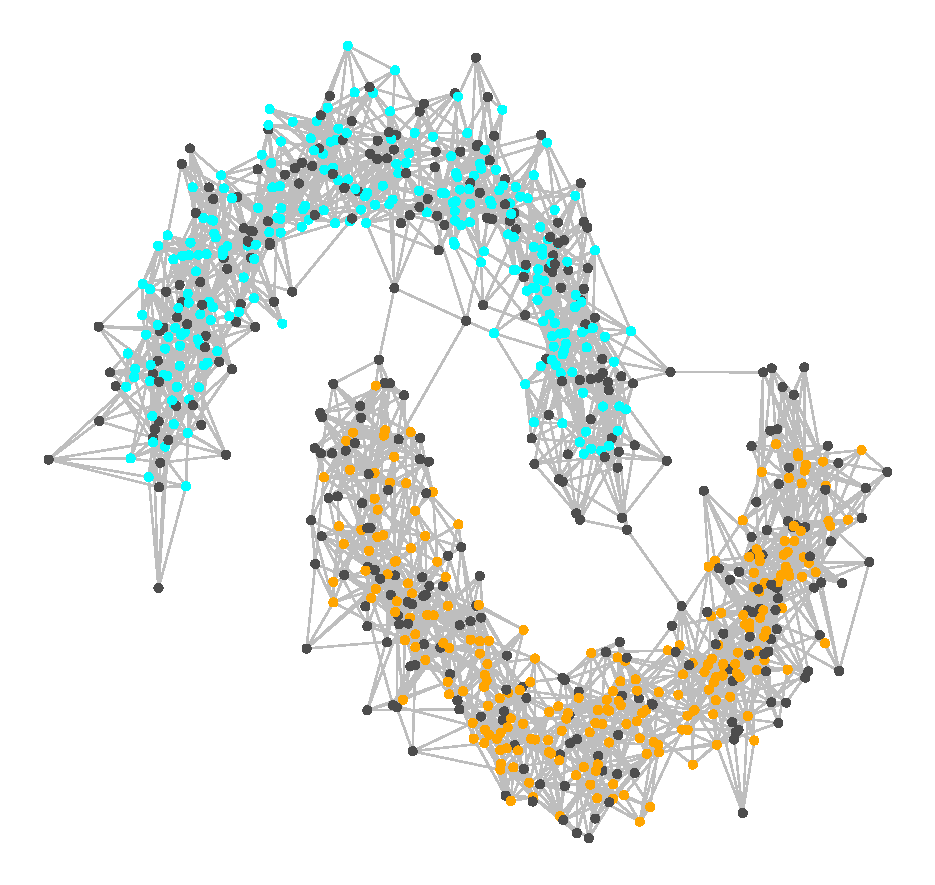
\includegraphics[width=\linewidth]{example2plots/row4_true_density_cluster}
			\caption{}
		\end{subfigure}
		\begin{subfigure}{.24\linewidth}
			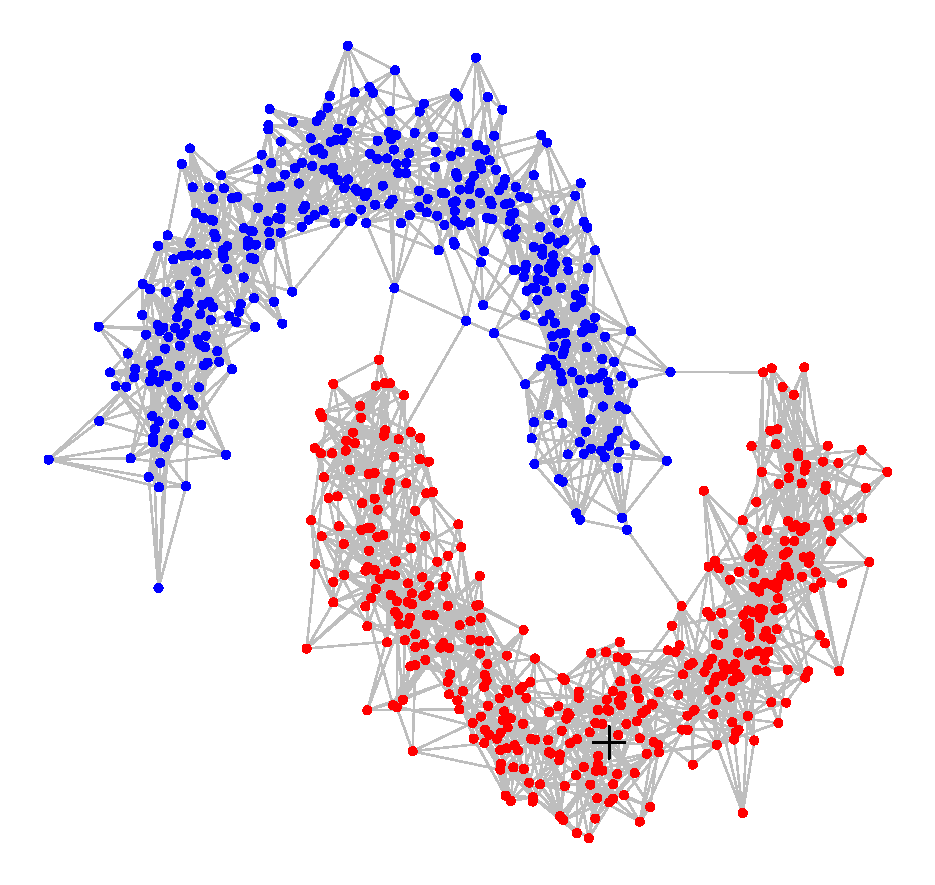
\includegraphics[width=\linewidth]{example2plots/row4_ppr_cluster}
			\caption{}
		\end{subfigure}
		\begin{subfigure}{.24\linewidth}
			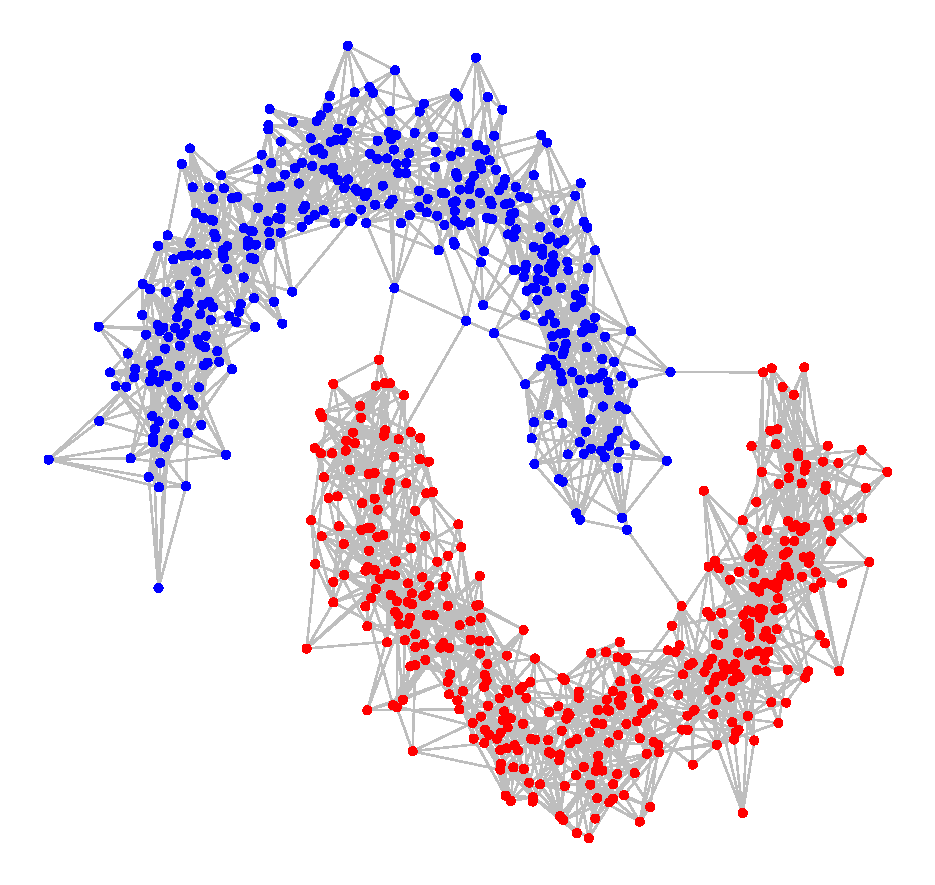
\includegraphics[width=\linewidth]{example2plots/row4_conductance_cluster}
			\caption{}
		\end{subfigure}
		\begin{subfigure}{.24\linewidth}
			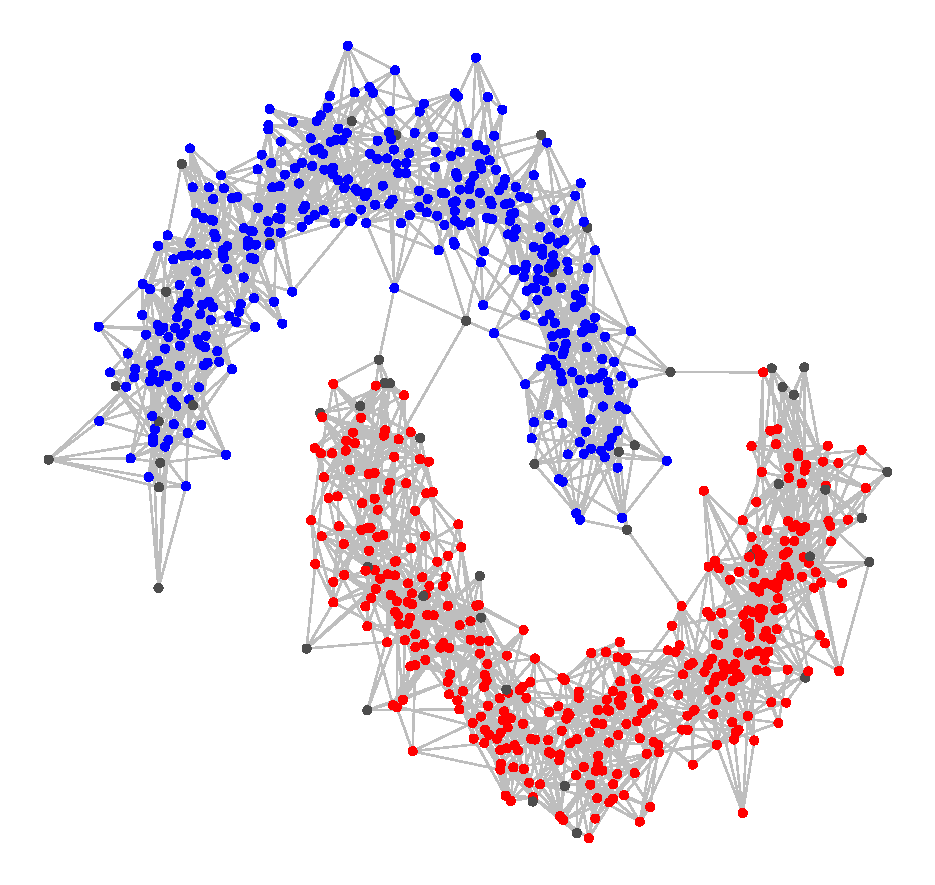
\includegraphics[width=\linewidth]{example2plots/row4_density_cluster}
			\caption{}
		\end{subfigure}
		\caption{}
		\label{fig:fig3}
	\end{adjustbox}
\end{figure}

\bibliographystyle{plainnat}
\bibliography{../local_spectral_bibliography}

\end{document}